\documentclass{report}

% Preamble: Include necessary packages
\usepackage[utf8]{inputenc}
\usepackage{amsmath}
\usepackage{graphicx}
\usepackage{array}
\usepackage{hyperref}
\usepackage{geometry}
\usepackage{setspace}
% Times 字体包在某些系统上可能缺少必要的字体文件
% 如果需要 Times 字体，请确保安装了 texlive-fontsrecommended 包
% \usepackage{times}
% \usepackage{newtxtext}
% \usepackage{newtxmath}
% \usepackage{mathptmx}
\usepackage{tocbibind}
\usepackage{listings}
\usepackage{xcolor}
\usepackage{booktabs}
\usepackage{multirow}
\usepackage{enumitem}
\usepackage{float}
\usepackage{tabularx}
\usepackage{longtable}
\usepackage{caption}
\usepackage{natbib}
\usepackage{tikz}
\usepackage{pgfplots}
\usepackage{pdfpages}




% \usepackage{pifont}  % 注释掉：系统缺少 pzdr 字体，且文档中未使用
% 定义 \ding 命令的替代方案
\newcommand{\ding}[1]{%
  \ifnum#1=55
    $\times$%  使用 × 符号替代 ding{55}
  \else
    \textbullet%  其他情况使用圆点
  \fi
}
\usepackage{array}
\usepackage{multirow}
\usepackage{amsmath}
\usepackage{amssymb}
\usepackage{graphicx}
\usepackage{xcolor}
\usepackage{caption}
% Configure packages
\pgfplotsset{compat=1.18}
\usetikzlibrary{mindmap, shapes.misc, positioning, calc, arrows.meta}

% Code listing style
\definecolor{codegreen}{rgb}{0,0.6,0}
\definecolor{codegray}{rgb}{0.5,0.5,0.5}
\definecolor{codepurple}{rgb}{0.58,0,0.82}
\definecolor{backcolour}{rgb}{0.95,0.95,0.92}

\lstdefinestyle{mystyle}{
    backgroundcolor=\color{backcolour},
    commentstyle=\color{codegreen},
    keywordstyle=\color{magenta},
    numberstyle=\tiny\color{codegray},
    stringstyle=\color{codepurple},
    basicstyle=\ttfamily\footnotesize,
    breakatwhitespace=false,
    breaklines=true,
    captionpos=b,
    keepspaces=true,
    numbers=left,
    numbersep=5pt,
    showspaces=false,
    showstringspaces=false,
    showtabs=false,
    tabsize=2
}
\lstset{style=mystyle}

% Page geometry
\geometry{
    a4paper,
    total={170mm,257mm},
    left=25mm,
    right=25mm,
    top=25mm,
    bottom=25mm
}

% Define title page elements
\title{Project Title Goes Here}
\author{Your Full Name \\ Your Student ID}
\date{\today}

\newcommand{\supervisor}{DR. CHIAM YIN KIA}
\newcommand{\university}{Universiti Malaya}
\newcommand{\faculty}{Faculty of Computer Science and Information Technology}
\newcommand{\department}{Software Engineering}
\newcommand{\studentname}{CAI HONGYI}
\newcommand{\studentid}{S2175463}
\newcommand{\programmecoursename}{WIA3002: ACADEMIC PROJECT I}
\newcommand{\stakeholder}{Infinity Datatech Sdn. Bhd.}

% 定义 frequirements 环境用于功能需求列表
\newenvironment{frequirements}{%
  \begin{enumerate}[nosep,leftmargin=*,topsep=0pt,partopsep=0pt]
}{%
  \end{enumerate}
}

% Begin document
\begin{document}

% ============================================================
% TITLE PAGE
% ============================================================
\begin{titlepage}
    \centering
    \vspace*{1cm}
      \begin{figure}
        \centering
        
\includegraphics[width=1\linewidth]{png2pdf.pdf}

        \label{fig:enter-label}
    \end{figure}
    {\Large \textbf{Final Year Project}} \\
    \vspace{1cm}
    {\Large \textbf{SEMESTER 1 2024/2025}} \\
    \vspace{2cm}
    {\Large \textbf{\MakeUppercase{Verdant-Search: AI-boosted Sharded Distributed Search Engine}}} \\
    \vspace{2cm}
    {\Large \textbf{SUPERVISOR:}} \\
    \vspace{0.5cm}
    {\Large \MakeUppercase{\supervisor}} \\
    \vspace{2cm}
    {\Large \textbf{PREPARED BY:}} \\
    \vspace{0.5cm}
    {\Large \MakeUppercase{\studentname}} \\
    \vspace{0.5cm}
    {\Large \MakeUppercase{\studentid}} \\
    \vfill
\end{titlepage}

% ============================================================
% ACKNOWLEDGEMENT
% ============================================================
\chapter*{Acknowledgement}
\addcontentsline{toc}{chapter}{Acknowledgement}

I would like to express my sincere gratitude to my academic supervisor, Dr. Chiam Yin Kia, for her invaluable guidance, insightful feedback, and unwavering support throughout the development of this project. Her expertise and mentorship have been instrumental in shaping both this work and my academic growth.

I extend my profound appreciation to Infinity Datatech Sdn. Bhd. for their collaboration and support as the industry partner for this project. Special thanks to the Chief Technology Officer and the Product Manager at Infinity Datatech, who generously shared their time, expertise, and insights during our numerous interviews and consultation sessions. Their willingness to explain their current workflows, challenges, and requirements has been essential in developing a solution that addresses real-world industry needs.

I am also grateful to the development and quality assurance teams at Infinity Datatech who participated in the requirements gathering sessions and provided valuable feedback during the system evaluation phase. Their practical insights have significantly contributed to the refinement of the platform's features and usability.

Finally, I would like to thank my family and friends for their continuous encouragement and support throughout my academic journey.

\clearpage

% ============================================================
% ABSTRACT
% ============================================================
\chapter*{Abstract}

Enterprise document collections contain rich multimodal content including charts, tables, and visual layouts, yet existing search systems rank documents based solely on text. Commercial solutions like Google Enterprise Search and Perplexity ignore visual information that often carries critical insights in business reports and technical documentation. Current retrieval augmented generation systems also operate exclusively on text, missing opportunities to leverage visual evidence or enable iterative search refinement where AI responses improve subsequent retrieval from corporate knowledge bases.

This work presents a production-ready enterprise search engine addressing these gaps through three core innovations. We develop a multimodal listwise reranker that extends methods like RankZephyr to jointly evaluate document text and visual layouts, enabling effective ranking of real-world business documents. Our iterative multimodal RAG framework creates a closed-loop system where LLM-generated insights refine subsequent searches through intelligent query rewriting, combining traditional search speed with AI reasoning capabilities. The end-to-end architecture prioritizes deployment efficiency through distributed crawling, compressed storage, and a two-stage pipeline where fast hybrid retrieval using BM25 inverted indexes and HNSW approximate nearest neighbor search identifies candidates, followed by expensive multimodal reranking on a focused set.

This system delivers capabilities absent in existing enterprise solutions: true image-text hybrid search, visually grounded question answering over business documents, and conversational refinement where each interaction improves retrieval quality. The architecture balances efficiency with effectiveness, achieving sub-second query latency on million-document collections while maintaining sophisticated cross-modal reasoning. By addressing practical gaps in multimodal reranking, enterprise RAG, and scalable deployment, this work provides both framework and implementation for next-generation enterprise search systems that naturally understand the full richness of modern business documents.
\clearpage

% ============================================================
% TABLE OF CONTENTS
% ============================================================
\tableofcontents
\clearpage

\listoftables
\clearpage

\listoffigures
\clearpage

% ============================================================
% CHAPTER 1: INTRODUCTION
% ============================================================
\chapter{Introduction}

\section{Background}

Modern web documents are fundamentally multimodal, with research papers containing critical diagrams, financial reports presenting data through visualizations, and technical documentation relying on architectural illustrations. Yet contemporary search engines remain text-centric, discarding visual content or treating images as disconnected entities. This limitation stems from historical constraints when processing images at scale was computationally prohibitive.

Recent advances have transformed what is feasible. Vision-language models like CLIP \cite{radford2021learning} and BLIP-2 \cite{li2023blip2} demonstrate effective joint reasoning over text and images through contrastive pretraining. Concurrently, large language models revolutionized document ranking through zero-shot listwise reranking, with RankGPT \cite{sun2023chatgpt} and RankZephyr \cite{pradeep2023rankzephyr} achieving state-of-the-art effectiveness by generating document permutations via prompting. However, these advances progress along parallel tracks: vision-language models focus on short image-caption matching while LLM-based rankers operate exclusively on text. No existing work performs listwise ranking over genuinely multimodal documents where relevance depends on understanding both textual and visual information. Furthermore, user interaction with search systems remains static, placing cognitive burden entirely on users for query refinement despite LLMs possessing sophisticated reasoning capabilities that could transform this paradigm \cite{lewis2020retrieval, asai2024self}.

\section{Problem Statement}

\textbf{Problem 1: Scalability Challenges for Enterprise Deployment.} Multimodal search requires expensive vision-language model inference for processing images alongside text, coordinated indexing across heterogeneous backends managing both inverted indexes and vector stores, and careful architectural optimization to achieve the subsecond query latency expected in interactive enterprise applications. Without strategic design choices balancing computational cost and ranking quality, multimodal search systems become impractical for deployment on large corporate document collections containing millions of items. The challenge lies in maintaining sophisticated cross-modal reasoning capabilities while meeting the performance requirements of production enterprise environments.

\textbf{Problem 2: Absence of Multimodal Reranking.} All existing learning-to-rank methods from classical approaches \cite{burges2005learning, cao2007learning} to recent LLM-based rerankers \cite{sun2023chatgpt, pradeep2023rankzephyr} process only text. No production-ready methods perform listwise reasoning over cross-modal evidence, assessing how document text and visual elements interact to convey information. While MMDocIR \cite{dong2025mmdocir} explored first-stage multimodal retrieval, the more impactful reranking stage remains unaddressed \cite{nogueira2019passage}. This gap prevents enterprise search systems from effectively ranking business documents where visual content quality, such as chart clarity and diagram effectiveness, significantly impacts document relevance.

\textbf{Problem 3: Limited Enterprise Knowledge Access and AI Integration.} Organizations require vertical search solutions that empower employees to efficiently access internal knowledge bases while leveraging AI assistance for comprehension and synthesis. However, existing systems lack bidirectional integration where search results improve AI-generated responses and AI-generated insights refine subsequent search queries. Traditional enterprise search presents static ranked lists, while current RAG implementations treat retrieval as one-shot preprocessing. Commercial solutions add AI summaries as passive overlays without feedback mechanisms, missing opportunities where conversational context and LLM reasoning about query intent could progressively improve retrieval quality within corporate knowledge bases through iterative refinement.

\section{Objective}

This project develops a production-ready multimodal search engine addressing these limitations through integrated solutions spanning system architecture, ranking algorithms, and conversational interaction. The objectives align with four core contributions.

\noindent\textbf{Objective 1: Scalable Multimodal Search Architecture.} Design and implement an enterprise-grade system supporting dual retrieval for text and images. The architecture employs distributed crawlers extracting content from corporate repositories, processes text queries through BM25 inverted indexes while simultaneously encoding queries via CLIP for HNSW-based image retrieval \cite{malkov2018efficient}. Key engineering challenges include distributed coordination across heterogeneous backends, incremental index updates, efficient query routing, and achieving subsecond latency for interactive enterprise applications.

\noindent\textbf{Objective 2: Iterative LLM-Guided Search Refinement.} Develop an interactive system with dual-interface presentation combining traditional ranked document lists with conversational AI summaries. The system implements a closed-loop search-RAG cycle where user follow-up questions trigger query rewriting incorporating conversation history, execute fresh multimodal retrieval and reranking, and generate refined summaries. The architecture balances query responsiveness with answer accuracy through strategic caching and incremental computation optimized for enterprise deployment.

\noindent\textbf{Objective 3: Multimodal Listwise Reranking.} Extend state-of-the-art listwise LLM ranking to multimodal business documents by adapting RankZephyr's sliding window and sorting methodology to jointly reason over text and visual content. The reranker employs vision-language models to assess cross-modal relationships including information consistency, contradiction detection, and complementarity evaluation. Setwise prompting is extended to multimodal scenarios where document comparisons jointly evaluate textual relevance and visual quality rather than independently fusing modality-specific scores.

\noindent\textbf{Objective 4: Comprehensive Empirical Evaluation.} Conduct extensive evaluation measuring multimodal reranking effectiveness across established benchmarks including TREC Deep Learning tracks \cite{craswell2020overview, craswell2021overview}, BEIR datasets \cite{thakur2021beir}, and MMDocIR \cite{dong2025mmdocir}. Baseline comparisons span BM25, CLIP-based retrieval, text-only listwise rerankers, and pairwise vision-language methods. Experiments systematically ablate visual information contribution, cross-modal interaction modeling, and architectural design choices while evaluating downstream impact on RAG-generated answer quality for enterprise knowledge retrieval tasks.

\section{Project Scope}

\subsection{System Scope}

The multimodal search engine encompasses the complete pipeline from document acquisition to result presentation, integrating retrieval, ranking, and generation components into a cohesive system.

\textbf{Distributed Web Crawling.} The system implements distributed crawlers that acquire web documents while extracting both textual content and associated images. Crawlers must respect robots.txt directives, implement polite crawling with configurable delays, handle dynamic content through JavaScript rendering when necessary, and coordinate across multiple worker nodes to maximize throughput while avoiding duplicate fetches. Extracted documents are parsed to identify text passages and linked images, with metadata including source URLs, timestamps, and document structure preserved for downstream processing.

\textbf{Hybrid Indexing Infrastructure.} Two parallel index structures support text and image retrieval respectively. The text index employs traditional inverted index data structures mapping terms to posting lists of documents containing those terms, supporting efficient BM25 scoring. The image index maintains CLIP embeddings for all extracted images in an HNSW graph structure enabling approximate nearest neighbor search with logarithmic query complexity. Both indexes must support incremental updates as new documents are crawled, with mechanisms ensuring consistency between text and image representations of the same document.

\textbf{Query Processing and Routing.} User queries are processed through both retrieval pathways simultaneously. Text queries are tokenized, stop words removed, and terms matched against the inverted index to retrieve candidate documents scored by BM25. The same query text is encoded by CLIP's text encoder and matched against image embeddings via HNSW traversal to retrieve visually relevant images with associated source documents. Results from both pathways are merged based on configurable fusion strategies before being passed to the reranking stage.

\textbf{Multimodal Reranking.} Candidate documents from first-stage retrieval, each potentially containing multiple images, are reranked using vision-language models that jointly assess textual and visual relevance. The reranker implements sliding window processing to handle top-k candidates exceeding model context limits, employing sorting algorithms to efficiently identify the most relevant documents without exhaustively comparing all pairs. Prompt engineering guides the vision-language model to evaluate cross-modal consistency, contradiction, and complementarity when scoring documents.

\textbf{Dual-Interface Presentation.} The user interface presents both a traditional ranked list of documents and a conversational panel displaying AI-generated summaries. The ranked list updates in real time as users refine queries through the conversational interface. When users pose follow-up questions, the system rewrites queries incorporating conversation history, triggers fresh retrieval and reranking, updates the document list, and generates new summaries grounded in the refined results. This closed-loop interaction continues until the user's information need is satisfied.

\subsection{Target Users}

The system is deployed within a VPN service provider organization to address knowledge management needs for internal technical teams and customer-facing support staff who require comprehensive access to product documentation, VPN technical knowledge, and censorship circumvention expertise.

\textbf{Internal Development Teams.} Software engineers and network architects require rapid access to technical documentation where network topology diagrams visually illustrate packet routing alongside textual specifications, and system metrics are presented through visualizations that complement log analysis. The multimodal search enables queries for configuration guides where architecture diagrams clearly show load balancer topologies, prioritizing documents where visual content substantively aids technical comprehension.

\textbf{Customer Service Representatives.} Support staff assisting users with VPN setup and troubleshooting require documents where screenshot sequences illustrate UI navigation steps and network diagrams show how obfuscation protocols bypass censorship. The conversational AI interface allows representatives to refine queries iteratively through natural language during live customer interactions, reducing the time cost of manual query reformulation while automatically incorporating conversation history.

\subsection{System Limitations}

\textbf{Computational and Scale Constraints.} Vision-language model inference requires GPU acceleration, limiting concurrent user capacity. The system implements periodic batch index updates rather than real-time streaming, and crawled corpus coverage focuses on technical documentation domains rather than comprehensive web coverage.

\textbf{Model Capability Boundaries.} Cross-modal understanding is bounded by vision-language models trained on image-caption pairs, which may struggle with relationships between lengthy passages and multiple images. The system is optimized for English-language documents, with potential effectiveness degradation on highly specialized domains. Evaluation benchmarks were not specifically designed for cross-modal ranking, introducing potential measurement artifacts.

\section{Project Schedule}

To be determined based on project timeline and milestone definitions.

% ============================================================
% CHAPTER 2: LITERATURE REVIEW
% ============================================================
\chapter{Literature Review}

\section{Search Engine Fundamentals and Architecture}

Modern information retrieval systems build upon decades of innovation. PageRank \cite{page1999pagerank} revolutionized web search by treating hyperlinks as quality indicators, establishing that relevance extends beyond textual matching. Brin and Page \cite{brin1998anatomy} formalized the tripartite architecture—crawlers, indexers, and query processors—that remains fundamental today.

The evolution from keyword matching to semantic understanding marks a critical transition. Early systems relied on lexical overlap \cite{baeza1999modern}, but neural approaches demonstrated that semantic comprehension yields superior retrieval \cite{mitra2017neural}. Dense Passage Retrieval \cite{karpukhin2020dense} showed BERT-based encoders capture semantic similarity in vector space, enabling relevant retrieval despite zero lexical overlap. This necessitated multi-stage pipelines where fast retrievers cast a wide net and slower rerankers refine results \cite{nogueira2019passage}.

Table \ref{tab:search_evolution} summarizes the key paradigm shifts in search engine development.

\begin{table}[h]
\centering
\caption{Evolution of Search Engine Paradigms}
\label{tab:search_evolution}
\begin{tabular}{llll}
\toprule
\textbf{Era} & \textbf{Method} & \textbf{Key Innovation} & \textbf{Limitation} \\
\midrule
1990s & Keyword Match & TF-IDF, BM25 & Lexical gap \\
2000s & Link Analysis & PageRank & Structure-only \\
2010s & Neural IR & BERT, Dense Retrieval & Computational cost \\
2020s & LLM-based & Zero-shot ranking & Efficiency challenges \\
\bottomrule
\end{tabular}
\end{table}

\section{Keyword-Based Search Methods}

Inverted indexes enable efficient keyword search at web scale \cite{zobel2006inverted}. By maintaining posting lists mapping terms to documents, they reduce search space from entire corpus to relevant candidates. This sparsity is critical for billion-scale collections with subsecond latency.

Term weighting determines keyword influence on relevance. TF-IDF \cite{sparck1972statistical, salton1975vector} balances term frequency against inverse document frequency, identifying discriminative terms. Salton and Buckley \cite{salton1988term} established that length normalization and frequency transformations significantly impact effectiveness.

BM25 \cite{robertson1994okapi, robertson2009probabilistic} emerged as the dominant probabilistic framework, introducing saturation functions and document length normalization:

\begin{equation}
\text{BM25}(q, d) = \sum_{t \in q} \text{IDF}(t) \cdot \frac{f(t, d) \cdot (k_1 + 1)}{f(t, d) + k_1 \cdot (1 - b + b \cdot \frac{|d|}{\text{avgdl}})}
\end{equation}

Despite neural advances, BM25 remains competitive on many benchmarks \cite{lin2021pretrained}. Contriever \cite{izacard2022unsupervised} demonstrates unsupervised contrastive learning can approach supervised neural retrieval, suggesting the classical-neural dichotomy is less stark than perceived.

\section{Vector Search and Neural Retrieval}

Dense vector representations enable semantic search transcending keyword matching. Early embeddings (Word2Vec \cite{mikolov2013efficient}, GloVe \cite{pennington2014glove}) captured word-level semantics. Transformers \cite{vaswani2017attention} elevated representation learning through self-attention, culminating in BERT \cite{devlin2019bert} with superior contextualized embeddings.

Sentence-BERT \cite{reimers2019sentence} adapted BERT for semantic similarity via siamese networks, enabling efficient similarity computation. ColBERT \cite{khattab2020colbert} refined this with late interaction—independent encoding but fine-grained token-level comparisons.

\begin{table}[h]
\centering
\caption{Approximate Nearest Neighbor Algorithms Comparison}
\label{tab:ann_comparison}
\begin{tabular}{llll}
\toprule
\textbf{Algorithm} & \textbf{Index Structure} & \textbf{Query Complexity} & \textbf{Trade-off} \\
\midrule
PQ \cite{jegou2011product} & Codebooks & O(N) & Memory vs. accuracy \\
HNSW \cite{malkov2018efficient} & Proximity graphs & O(log N) & Build time vs. query \\
IVF & Inverted file & O(N/k) & Partitions vs. recall \\
\bottomrule
\end{tabular}
\end{table}

ANN algorithms make dense retrieval tractable at scale (Table \ref{tab:ann_comparison}). Product Quantization \cite{jegou2011product} compresses vectors via learned codebooks. HNSW \cite{malkov2018efficient} constructs multi-layer proximity graphs enabling logarithmic search. ANCE \cite{xiong2021approximate} demonstrated iterative hard negative mining substantially improves retrieval quality. BEIR \cite{thakur2021beir} revealed MS MARCO-optimized models often struggle out-of-domain, highlighting generalization challenges.

\section{Learning-to-Rank Approaches}

Learning-to-Rank formulates ranking as supervised learning on query-document relevance judgments \cite{liu2009learning}. Three paradigms emerged based on learning signal granularity: pointwise (independent relevance prediction), pairwise (relative preferences), and listwise (direct metric optimization).

\begin{table}[h]
\centering
\caption{Learning-to-Rank Paradigms Comparison}
\label{tab:ltr_paradigms}
\small
\begin{tabular}{lllll}
\toprule
\textbf{Paradigm} & \textbf{Method} & \textbf{Loss} & \textbf{Strength} & \textbf{Weakness} \\
\midrule
Pointwise & Regression & MSE & Simple & Ignores order \\
Pairwise & RankNet \cite{burges2005learning} & Pairwise CE & Relative & Quadratic pairs \\
 & LambdaRank \cite{burges2006learning} & NDCG gradient & Direct metric & Complex \\
 & LambdaMART \cite{burges2010ranknet} & Boosted trees & Robust & Feature eng. \\
Listwise & ListNet \cite{cao2007learning} & Top-one prob. & Full list & Permutation cost \\
 & ListMLE \cite{xia2008listwise} & MLE & Principled & Computational \\
\midrule
\multicolumn{5}{l}{\textit{LLM-based Zero-shot (no training data required)}} \\
Listwise & RankGPT \cite{sun2023chatgpt} & Generation & Zero-shot & Cost, latency \\
 & RankZephyr \cite{pradeep2023rankzephyr} & Setwise & Efficient & Needs logits \\
Pairwise & Pairwise LLM \cite{qin2023pairwise} & Comparison & Effective & Quadratic cost \\
\bottomrule
\end{tabular}
\end{table}

Pointwise methods treat ranking as regression but ignore relative ordering. Pairwise methods learn preferences: RankNet \cite{burges2005learning} pioneered neural pairwise ranking; LambdaRank \cite{burges2006learning} directly optimized NDCG via gradient manipulation; LambdaMART \cite{burges2010ranknet} combined LambdaRank gradients with gradient-boosted trees, dominating for over a decade.

Listwise methods optimize ranking metrics over entire lists. ListNet \cite{cao2007learning} introduced top-one probability models; ListMLE \cite{xia2008listwise} formulated ranking as maximum likelihood over permutations.

NDCG \cite{jarvelin2000ir, jarvelin2002cumulated} became the standard metric through position-dependent discounting:
\begin{equation}
\text{NDCG}@k = \frac{\text{DCG}@k}{\text{IDCG}@k}, \quad \text{DCG}@k = \sum_{i=1}^{k} \frac{2^{\text{rel}_i} - 1}{\log_2(i + 1)}
\end{equation}

Large language models revolutionized learning-to-rank through zero-shot reranking via prompting. RankGPT \cite{sun2023chatgpt} demonstrated GPT-4 can rerank documents by generating permutations, achieving competitive effectiveness without task-specific training. RankZephyr \cite{pradeep2023rankzephyr} distilled GPT-4 behavior into smaller models via instruction tuning, introducing setwise prompting that compares multiple documents simultaneously, substantially reducing inference cost. However, these listwise LLM rerankers operate exclusively on text, unexplored for multimodal content.

\section{Multimodal Search and Retrieval}

Vision-language pretraining enables joint image-text representations. CLIP \cite{radford2021learning} trained contrastively on 400M image-caption pairs, aligning visual and linguistic semantics for zero-shot classification and retrieval. ALIGN \cite{jia2021scaling} demonstrated scaling to noisier but larger datasets improves alignment. ALBEF \cite{li2021align} introduced momentum distillation; BLIP \cite{li2022blip} unified understanding and generation; BLIP-2 \cite{li2023blip2} connected frozen image encoders to LLMs via lightweight transformers.

\begin{table}[h]
\centering
\caption{Vision-Language Models for Multimodal Retrieval}
\label{tab:vlm_comparison}
\small
\begin{tabular}{llllll}
\toprule
\textbf{Model} & \textbf{Year} & \textbf{Training Data} & \textbf{Modality} & \textbf{Task} & \textbf{Zero-shot} \\
\midrule
CLIP \cite{radford2021learning} & 2021 & 400M pairs & Image + Text & Retrieval & \checkmark \\
ALIGN \cite{jia2021scaling} & 2021 & 1.8B noisy & Image + Text & Retrieval & \checkmark \\
ALBEF \cite{li2021align} & 2021 & 14M pairs & Image + Text & Both & \checkmark \\
BLIP \cite{li2022blip} & 2022 & 129M pairs & Image + Text & Both & \checkmark \\
BLIP-2 \cite{li2023blip2} & 2023 & 129M pairs & Image + Text + LLM & Both & \checkmark \\
\midrule
MMDocIR \cite{dong2025mmdocir} & 2025 & 313 docs & Page + Layout & Retrieval & \ding{55} \\
\bottomrule
\end{tabular}
\end{table}

Despite advances in multimodal representation, document retrieval applications remain limited. Existing models focus on image-caption scenarios with short text, whereas documents involve lengthy passages where images illustrate rather than dominate. MMDocIR \cite{dong2025mmdocir} benchmarked multimodal retrieval for long documents, introducing page-level and layout-level tasks across 313 documents spanning 10 domains. Vision-driven retrievers significantly outperform text-only methods, especially capturing visual semantics OCR fails to preserve. However, \textbf{MMDocIR focused exclusively on first-stage retrieval, leaving the more impactful reranking stage unexplored for multimodal content.}

Cross-modal retrieval employs early fusion (joint encoding) or late fusion (separate encoding, late combination). Early fusion enables fine-grained interaction but sacrifices scalability. Late fusion permits efficient ANN search but loses interaction. Multi-modal tensor fusion \cite{wang2019matching} explores intermediate architectures balancing interaction and efficiency, though not widely adopted for web-scale retrieval.

\section{Retrieval-Augmented Generation}

RAG bridges information retrieval and generation by grounding LLM outputs in retrieved evidence \cite{lewis2020retrieval}, addressing knowledge limitations and hallucination. REALM \cite{guu2020retrieval} pioneered joint retriever-generator training through end-to-end backpropagation with differentiable document indexes.

Standard RAG treats retrieval as one-shot preprocessing—query, retrieve documents, generate answer conditioned on concatenated passages. This fails to leverage LLM reasoning for improving retrieval. Self-RAG \cite{asai2024self} introduced self-reflection where models generate critique tokens assessing passage support and triggering adaptive retrieval. CRAG \cite{yan2024corrective} extended this with corrective strategies—evaluators assess document relevance and trigger web search when initial retrieval is inadequate. However, both treat retrievers as black boxes unable to benefit from LLM-generated insights.

\begin{table}[h]
\centering
\caption{RAG System Design Dimensions}
\label{tab:rag_design}
\small
\begin{tabular}{lll}
\toprule
\textbf{Dimension} & \textbf{Options} & \textbf{Trade-off} \\
\midrule
Retrieval Frequency & One-shot, Iterative & Latency vs. quality \\
Chunk Granularity & Sentence, Paragraph, Document & Context vs. precision \\
Integration Strategy & Concatenation, Attention & Simplicity vs. interaction \\
Modality & Text-only, Multimodal & Coverage vs. complexity \\
\bottomrule
\end{tabular}
\end{table}

Recent surveys \cite{gao2023retrieval} systematically analyzed RAG architectures, identifying key design dimensions (Table \ref{tab:rag_design}). However, practical guidance for specific applications remains limited. \textbf{RAG application to multimodal retrieval has received minimal attention, with existing work focusing almost exclusively on text-only scenarios} despite many real-world needs spanning text and images.

Conversational search \cite{mo2024survey} considers information seeking as interactive dialogue. This demands systems maintain conversation history and understand follow-up query relationships. Conversational RAG must ground responses in retrieved evidence while supporting natural dialogue. Current approaches use query rewriting to incorporate history into standalone retrieval queries, \textbf{but do not close the loop by using generated insights to improve subsequent retrieval.}

\section{Benchmark Datasets and Evaluation}

MS MARCO \cite{nguyen2016ms} established large-scale retrieval benchmarks with 1M queries from real Bing logs. TREC Deep Learning Tracks \cite{craswell2020overview, craswell2021overview, craswell2022overview} extended MS MARCO with densely judged test sets, enabling reliable measurement and reducing pool bias.

\begin{table}[h]
\centering
\caption{Major IR Benchmark Datasets Comparison}
\label{tab:benchmark_comparison}
\small
\begin{tabular}{lllll}
\toprule
\textbf{Dataset} & \textbf{Queries} & \textbf{Documents} & \textbf{Domain} & \textbf{Modality} \\
\midrule
MS MARCO v1 & 1M train, 6.9K test & 8.8M & Web & Text \\
MS MARCO v2 & Similar & 138M & Web & Text \\
TREC DL 19-22 & 200-600/yr & From MS MARCO & Web & Text \\
BEIR (18 sets) & Varies & Varies & Multi-domain & Text \\
NovelEval & Continuous & Continuous & Web & Text \\
\midrule
MMDocIR & 1.7K expert & 313 docs (65 pages avg) & 10 domains & Text + Image \\
\bottomrule
\end{tabular}
\end{table}

BEIR \cite{thakur2021beir} addressed generalization limitations by assembling 18 diverse datasets (Table \ref{tab:benchmark_comparison}). Zero-shot evaluation revealed many neural retrievers suffer dramatic out-of-domain drops, highlighting brittleness. This has particular implications for multimodal retrieval where visual content varies more dramatically than text.

Evaluation methodology requires careful consideration of measurement reliability and statistical testing. NDCG has become standard due to handling graded relevance with position-dependent discounting. However, metrics assume complete, accurate judgments—rarely true due to pooling limitations and annotator disagreement. MS MARCO leaderboard design requires careful engineering to prevent gaming while enabling broad participation \cite{craswell2021msmarco}.

NovelEval specifically addresses data contamination by continuously updating test queries to include only those arising after model training cutoffs, ensuring measurements reflect generalization rather than memorization. \textbf{For multimodal ranking, establishing similar contamination-free benchmarks is critical} given vision-language models train on massive web-scraped datasets potentially overlapping evaluation sets.

\section{Research Gaps and Opportunities}

Despite significant progress in multimodal representation learning and LLM-based ranking, critical gaps remain:

\textbf{Gap 1: Multimodal Reranking.} All existing learning-to-rank methods operate exclusively on text. While MMDocIR demonstrated visual information value for first-stage retrieval, \textbf{the reranking stage where cross-encoders prove most impactful remains unexplored for multimodal content.} This represents significant opportunity given rerankers can afford expensive cross-modal reasoning first-stage retrievers cannot.

\textbf{Gap 2: Multimodal RAG.} The interaction between multimodal retrieval and generation has received minimal attention. RAG systems assume text-only retrieval and generation, failing to leverage visual evidence that could improve answer quality for visually grounded questions. The converse opportunity exists where generated natural language explanations of multimodal content could improve retrieval by providing richer training signal than sparse labels typically available.

\textbf{Gap 3: Multimodal Evaluation Infrastructure.} Robust evaluation of multimodal ranking systems requires datasets with ground truth relevance judgments spanning text and images, which do not currently exist at scale. Extending existing benchmarks like MS MARCO with visual content and collecting relevance judgments accounting for cross-modal interactions would enable rigorous assessment. This evaluation infrastructure is prerequisite for driving multimodal ranking research progress.

\textbf{Gap 4: Efficiency-Effectiveness Balance.} The efficiency of multimodal ranking deserves careful consideration given computational cost of vision-language models. While RankZephyr demonstrated setwise prompting can substantially reduce inference cost for text-only ranking, extending this to multimodal content where each candidate includes both text and images will amplify computational demands. Developing efficient multimodal reranking architectures balancing effectiveness with practical deployment constraints represents an important open problem.

\textbf{Gap 5: Iterative Multimodal Search.} Current search systems, even those with RAG, do not support iterative refinement where LLM-generated insights feedback into subsequent multimodal retrieval. This closed-loop approach where search results drive LLM generation, which in turn refines search queries, remains unexplored for multimodal content.

\section{Proposed Approach: Multimodal LTR-Enhanced Search Engine}

\begin{table}[h]
\centering
\caption{System Capabilities Comparison: Proposed vs. Existing Approaches}
\label{tab:system_comparison}
\footnotesize
\setlength{\tabcolsep}{3pt}
\renewcommand{\arraystretch}{1.1}
\begin{tabular}{l@{\hspace{4pt}}c@{\hspace{3pt}}c@{\hspace{3pt}}c@{\hspace{3pt}}c@{\hspace{3pt}}c@{\hspace{3pt}}c}
\toprule
\textbf{Capability} & \rotatebox{60}{\textbf{Ours}} & \rotatebox{60}{\textbf{Google}} & \rotatebox{60}{\textbf{Perplexity}} & \rotatebox{60}{\textbf{MMDocIR}} & \rotatebox{60}{\textbf{RankZephyr}} & \rotatebox{60}{\textbf{Traditional IR}} \\
\midrule
\multicolumn{7}{l}{\textit{\textbf{Retrieval Capabilities}}} \\
Keyword Search (Inverted Index) & \checkmark & \checkmark & \checkmark & \checkmark & \ding{55} & \checkmark \\
Semantic Search (Dense Vectors) & \checkmark & \checkmark & \checkmark & \checkmark & \ding{55} & \ding{55} \\
Hybrid Retrieval & \checkmark & \checkmark & \checkmark & \ding{55} & \ding{55} & \ding{55} \\
Image+Text Multimodal Retrieval & \checkmark & \checkmark & \ding{55} & \checkmark & \ding{55} & \ding{55} \\
Efficient ANN (HNSW) & \checkmark & \checkmark & \checkmark & \ding{55} & \ding{55} & \ding{55} \\
\midrule
\multicolumn{7}{l}{\textit{\textbf{Ranking Capabilities}}} \\
First-Stage Ranking & \checkmark & \checkmark & \checkmark & \checkmark & \checkmark & \checkmark \\
Second-Stage Reranking & \checkmark & \checkmark & \checkmark & \ding{55} & \checkmark & \ding{55} \\
Multimodal LTR Reranker & \checkmark & ? & \ding{55} & \ding{55} & \ding{55} & \ding{55} \\
Listwise Ranking & \checkmark & ? & \ding{55} & \ding{55} & \checkmark & \ding{55} \\
\midrule
\multicolumn{7}{l}{\textit{\textbf{Generation \& Interaction}}} \\
LLM Integration & \checkmark & \checkmark & \checkmark & \ding{55} & \ding{55} & \ding{55} \\
RAG-based Summarization & \checkmark & \checkmark & \checkmark & \ding{55} & \ding{55} & \ding{55} \\
Conversational Refinement & \checkmark & \checkmark & \checkmark & \ding{55} & \ding{55} & \ding{55} \\
Iterative Search Feedback Loop & \checkmark & \ding{55} & \ding{55} & \ding{55} & \ding{55} & \ding{55} \\
Query Rewriting from Context & \checkmark & \checkmark & \checkmark & \ding{55} & \ding{55} & \ding{55} \\
\midrule
\multicolumn{7}{l}{\textit{\textbf{System Architecture}}} \\
Distributed Crawling & \checkmark & \checkmark & \ding{55} & \ding{55} & \ding{55} & \checkmark \\
Compressed Storage & \checkmark & \checkmark & ? & \ding{55} & \ding{55} & \ding{55} \\
Dual-Panel UI (Search + AI) & \checkmark & \checkmark & \checkmark & \ding{55} & \ding{55} & \ding{55} \\
Real-time Index Updates & \checkmark & \checkmark & ? & \ding{55} & \ding{55} & \ding{55} \\
\midrule
\multicolumn{7}{l}{\textit{\textbf{Evaluation \& Research}}} \\
Benchmark Contribution & \checkmark & \ding{55} & \ding{55} & \checkmark & \checkmark & \ding{55} \\
Open Source & \checkmark & \ding{55} & \ding{55} & \checkmark & \checkmark & Varies \\
Research Focus & All stages & Production & Production & First-stage & Reranking & Traditional \\
\bottomrule
\end{tabular}
\end{table}

\subsection{Key Innovations}

Our system makes four key contributions addressing identified gaps:

\textbf{1. Multimodal Listwise Reranker:} First work to apply listwise LTR to multimodal content, extending RankZephyr's setwise prompting to handle image+text candidates. This addresses Gap 1 by bringing the most effective reranking paradigm to multimodal scenarios.

\textbf{2. Iterative Multimodal RAG:} LLM-generated insights feed back into subsequent multimodal retrieval, creating a closed loop where search results drive generation, which refines search. This addresses Gap 5 by enabling conversational refinement that updates both document rankings and AI responses.

\textbf{3. End-to-End Multimodal Pipeline:} Complete system from distributed crawling through compressed storage, hybrid retrieval (keyword+semantic), two-stage ranking (ANN first-stage, LTR reranking), to RAG generation. This integrates state-of-the-art components across the full pipeline.

\textbf{4. Efficiency-Effectiveness Balance:} Strategic use of HNSW for efficient ANN, compressed storage for scalability, and optimized multimodal reranking for practical deployment. This addresses Gap 4 by making multimodal reranking computationally feasible.

As Table \ref{tab:system_comparison} demonstrates, our system is the only approach combining multimodal retrieval, multimodal reranking, and iterative LLM-driven refinement in a complete end-to-end architecture. This positions our work to make significant contributions to both multimodal information retrieval research and practical search system development.

% ============================================================
% CHAPTER 3: RESEARCH METHODOLOGY
% ============================================================
\chapter{Research Methodology}
This chapter outlines the methodological approach used to develop the Verdant Search multimodal enterprise search engine for Infinity Datatech, detailing the software development lifecycle and the comprehensive data gathering techniques employed to define requirements and validate design decisions.

\section{Software Development Methodology}

To effectively navigate the dynamic requirements of building a novel multimodal search platform in close collaboration with an industry partner, this project adopted an Agile development methodology. Agile is a modern approach to project management and software development that emphasizes flexibility, customer collaboration, and iterative progress. Unlike traditional, linear approaches (like Waterfall) where requirements are fixed upfront, Agile embraces change and allows for requirements to evolve through a continuous feedback loop between the developer and stakeholders. This was particularly suitable for this academic-industry partnership where the complexity of integrating distributed crawling, hybrid retrieval, and multimodal reranking required frequent validation cycles.

The core philosophy of Agile is centered on delivering value in small, incremental pieces, enabling rapid validation and adaptation throughout the project lifecycle. This iterative nature was crucial for ensuring the search engine met the precise and evolving needs of Infinity Datatech's technical teams, allowing for early detection of issues and continuous alignment with the company's enterprise knowledge management goals.

\begin{figure}[H]
\centering
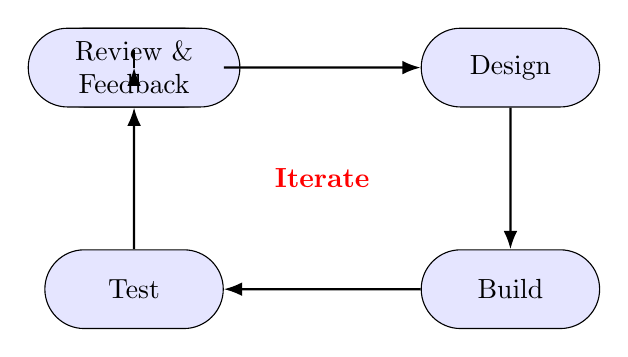
\begin{tikzpicture}[node distance=1.8cm and 2.5cm,
every node/.style={draw, rounded rectangle, text centered, minimum height=1cm, minimum width=2.5cm, text width=2.2cm, fill=blue!10},
arrow/.style={-Latex, thick}]
    \node (plan) {Plan};
    \node (design) [right=of plan] {Design};
    \node (build) [below=of design] {Build};
    \node (test) [left=of build] {Test};
    \node (review) [above=of test] {Review \& Feedback};
    
    \draw[arrow] (plan) -- (design);
    \draw[arrow] (design) -- (build);
    \draw[arrow] (build) -- (test);
    \draw[arrow] (test) -- (review);
    \draw[arrow] (review) to[bend left=15] (plan);
    
    \node[draw=none, fill=none, font=\bfseries, text=red] at ($(plan)!0.5!(build)$) {Iterate};
\end{tikzpicture}
\caption{The Agile Iterative Development Cycle}
\label{fig:agile_cycle}
\end{figure}


\subsection{Implementing the Scrum Framework}
To provide structure to the Agile approach, the project was managed using Scrum, a popular and effective Agile framework. Scrum organizes work into fixed-length iterations called Sprints, which in this project were set to two weeks. Each Sprint is a self-contained mini-project that results in a demonstrable and potentially usable increment of the final search engine system.

The Scrum framework consists of key roles, artifacts (documents/tools), and events (meetings) that guided the project:

\subsubsection{Scrum Roles}
\begin{itemize}
\item \textbf{Product Owner:} Key stakeholders at Infinity Datatech, primarily the Product Manager and technical leads, who defined the project vision and prioritized features based on organizational knowledge management needs.
\item \textbf{Development Team:} A self-contained role filled by the sole developer on this academic project, responsible for building the full-stack search engine system including distributed crawling, indexing pipeline, and frontend interface.
\item \textbf{Scrum Master:} A dual role fulfilled by the developer (for process facilitation) and the academic supervisor (for guidance and impediment removal), ensuring the Scrum framework was followed effectively and academic standards were met.
\end{itemize}

\subsubsection{Scrum Artifacts}
\begin{itemize}
\item \textbf{Product Backlog:} A master list of all features and requirements, prioritized in collaboration with Infinity Datatech based on technical value and enterprise search needs. Items ranged from core retrieval functionality to advanced features like multimodal reranking and iterative RAG.
\item \textbf{Sprint Backlog:} A subset of high-priority tasks selected from the Product Backlog to be completed within a two-week Sprint, such as implementing the BM25 indexer or integrating CLIP embeddings.
\item \textbf{Increment:} The tangible, working, and tested piece of software produced at the end of each Sprint, adding to previous functionality with deployable search components. For example, one Sprint's increment might be the hybrid retrieval module, while the next might add the conversational query rewriting feature.
\end{itemize}

\subsubsection{Scrum Events}
The work was structured around a series of recurring events within each Sprint to ensure transparency and inspection:
\begin{enumerate}
\item \textbf{Sprint Planning:} Selecting items from the Product Backlog to define the Sprint Goal for search engine components.
\item \textbf{Daily Check-ins:} Brief, regular syncs to discuss progress and obstacles in development.
\item \textbf{Sprint Review:} A demonstration of the Sprint's increment to Infinity Datatech stakeholders to gather critical feedback on search quality and system performance.
\item \textbf{Sprint Retrospective:} An internal reflection to identify process improvements for the next Sprint.
\end{enumerate}

\begin{figure}[H]
\centering
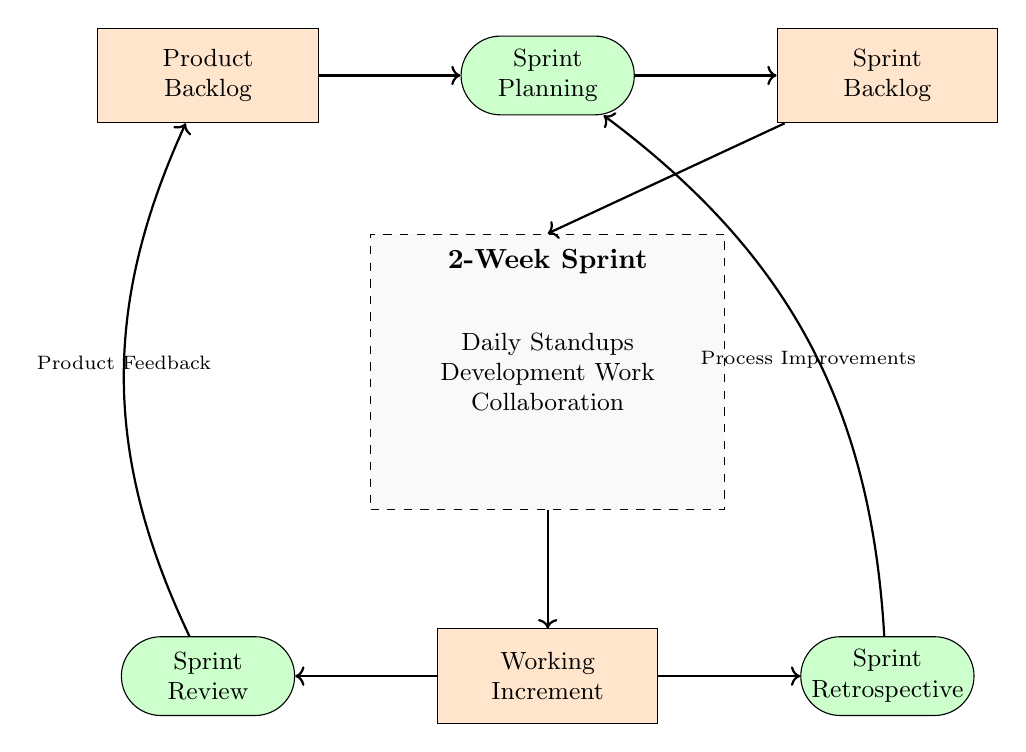
\begin{tikzpicture}[
artifact/.style={rectangle, draw, fill=orange!20, minimum height=1.2cm, minimum width=2.8cm, align=center, font=\small},
event/.style={rectangle, draw, fill=green!20, minimum height=1cm, minimum width=2.2cm, align=center, font=\small, rounded corners=0.5cm},
arrow/.style={->, thick},
sprint/.style={rectangle, draw, dashed, fill=gray!5, minimum height=3.5cm, minimum width=4.5cm}
]

% Top row - Planning phase
\node[artifact] (product_backlog) {Product\\Backlog};
\node[event, right=1.8cm of product_backlog] (sprint_planning) {Sprint\\Planning};
\node[artifact, right=1.8cm of sprint_planning] (sprint_backlog) {Sprint\\Backlog};

% Sprint box
\node[sprint, below=1.5cm of sprint_planning] (sprint_container) {};
\node[font=\bfseries] at ([yshift=1.4cm]sprint_container.center) {2-Week Sprint};
\node[font=\small, align=center] at (sprint_container.center) {Daily Standups\\Development Work\\Collaboration};

% Bottom row - Review phase  
\node[artifact, below=1.5cm of sprint_container] (increment) {Working\\Increment};
\node[event, left=1.8cm of increment] (sprint_review) {Sprint\\Review};
\node[event, right=1.8cm of increment] (retrospective) {Sprint\\Retrospective};

% Main flow arrows
\draw[arrow] (product_backlog) -- (sprint_planning);
\draw[arrow] (sprint_planning) -- (sprint_backlog);
\draw[arrow] (sprint_backlog) -- (sprint_container.north);
\draw[arrow] (sprint_container.south) -- (increment);
\draw[arrow] (increment) -- (sprint_review);
\draw[arrow] (increment) -- (retrospective);

% Feedback loops
\draw[arrow, bend left=25] (sprint_review) to node[above, font=\scriptsize] {Product Feedback} (product_backlog);
\draw[arrow, bend right=25] (retrospective) to node[below, font=\scriptsize] {Process Improvements} (sprint_planning);

\end{tikzpicture}
\caption{The Scrum Framework - Clear Process Flow}
\label{fig:scrum_framework}
\end{figure}

\subsection{Project Management and Workflow Tools}
To support this Agile Scrum process, a specific set of digital tools was employed:
\begin{itemize}
\item \textbf{GitHub:} Used for version control and managing the \textbf{Product} and \textbf{Sprint Backlogs} via Projects and Issues features for tracking search engine development. Each module (crawling, indexing, retrieval, reranking, RAG) was tracked as separate epics.
\item \textbf{Microsoft Teams:} Used for formal academic supervision meetings.
\item \textbf{Lark:} Serves as the central collaboration hub for daily communication, task tracking, and sprint management, coordinating distributed system components and data ingestion pipelines.
\end{itemize}


\section{Data Gathering Techniques}
To ensure the search engine met Infinity Datatech's specific requirements and addressed the inefficiencies of their current fragmented search processes, a comprehensive data gathering approach was employed. This combined multiple qualitative and quantitative methods, with a focus on understanding existing workflows, information retrieval needs, and stakeholder pain points. A key initial finding was that engineers spend significant time (30-45 minutes daily) searching across fragmented systems including Confluence, Google Drive, Git repositories, and local network shares. This fragmentation, combined with the inability to search visual content in technical documents, formed the core problems the new platform needed to solve.

\subsection{Literature Review}
The literature review (detailed in Chapter 2) explored existing academic research and industry practices in search engine architecture, learning-to-rank, vision-language models, and retrieval-augmented generation. This foundation was supplemented with:

\begin{itemize}
    \item Analysis of search engine architectures combining inverted indexes with dense retrieval, particularly hybrid approaches using BM25 and neural embeddings.
    \item Evaluation of existing commercial and open-source solutions (Google Enterprise Search, Perplexity, Elasticsearch) to assess their suitability for Infinity Datatech's multimodal search requirements.
    \item Examination of current approaches to LLM-based ranking (RankGPT, RankZephyr) and their potential extension to multimodal content.
\end{itemize}

\subsection{Stakeholder Interviews}
A series of structured and semi-structured interviews were conducted with key stakeholders at Infinity Datatech. These interviews were crucial for understanding strategic goals, operational pain points associated with current search processes, and specific requirements for an enterprise search solution.

\begin{table}[H]
\centering
\caption{Product Manager Interview Summary - Requirements Discovery}
\label{tab:pm_interview}
\begin{tabularx}{\textwidth}{|l|c|X|}
\hline
\textbf{Role} & \textbf{Sessions} & \textbf{Key Information Gathered} \\ 
\hline
Product Manager & 3 & Current search workflows, pain points (fragmented systems, terminology variations), feature priorities, and success metrics for enterprise search.

\textbf{Example Q:} ``Can you describe the current challenges your technical teams face when searching for internal documentation?''

\textbf{Outcome:} Engineers spend 30-45 minutes daily searching across fragmented systems (Confluence, Google Drive, Git repositories, local shares). Existing keyword search misses conceptually related documents due to terminology variations. Critical visual information in charts and diagrams is not searchable, forcing manual document browsing. No unified interface, requiring context switching between multiple tools.

\textbf{Example Q:} ``What types of queries do your teams typically need answers for?''

\textbf{Outcome:} Technical how-to questions requiring code examples and architecture diagrams. Troubleshooting queries needing logs, error messages, and past incident reports. Policy and compliance questions requiring exact citations. Comparative analysis requiring synthesis across multiple technical specifications. This revealed need for both precise retrieval and intelligent summarization. \\
\hline
\end{tabularx}
\end{table}

\begin{table}[H]
\centering
\caption{Product Manager Interview Summary - Feature Priorities}
\label{tab:pm_priorities}
\begin{tabularx}{\textwidth}{|l|c|X|}
\hline
\textbf{Role} & \textbf{Sessions} & \textbf{Key Information Gathered} \\ 
\hline
Product Manager & (continued) & Feature prioritization and evaluation criteria.

\textbf{Example Q:} ``If you had to prioritize three capabilities for the search system, what would they be?''

\textbf{Outcome:} \textbf{Priority 1:} Multimodal search that can find documents based on visual content descriptions, not just text. \textbf{Priority 2:} Conversational interface where follow-up questions refine results without starting over. \textbf{Priority 3:} Source attribution with exact citations so answers can be verified and trusted. Additional need: Sub-second query response time for daily usage adoption.

\textbf{Example Q:} ``How do you currently evaluate whether search results are relevant?''

\textbf{Outcome:} Manual inspection of top 10 results for precision. User feedback on whether they found what they needed. Time to complete search task as efficiency metric. This informed our evaluation methodology using NDCG@10, MRR, and latency measurements. \\
\hline
\end{tabularx}
\end{table}

\begin{table}[H]
\centering
\caption{Technical Team Lead Interview Summary}
\label{tab:tech_interview}
\begin{tabularx}{\textwidth}{|l|c|X|}
\hline
\textbf{Role} & \textbf{Sessions} & \textbf{Key Information Gathered} \\ 
\hline
Technical Lead & 2 & Infrastructure requirements, data source integration, performance constraints.

\textbf{Example Q:} ``What data sources need to be indexed, and what are the access patterns?''

\textbf{Outcome:} Primary sources include Confluence (REST API access), Google Drive (Drive API), Git repositories (Git protocol), and local network shares (SMB/NFS). Documents range from technical specifications to incident reports, with many containing critical charts and diagrams.

\textbf{Example Q:} ``What are the performance expectations for a production search system?''

\textbf{Outcome:} P90 latency under 4 seconds from query to complete response. System must scale to 10 million document index. Must integrate with internal identity providers for access control. \\
\hline
\end{tabularx}
\end{table}

Interview protocols were developed to systematically explore:

\begin{itemize}
    \item Current search processes and challenges, specifically the fragmentation across multiple data sources (Confluence, Google Drive, Git, file shares).
    \item Information retrieval patterns and the types of queries teams need answered.
    \item Key metrics for search quality: \textbf{precision, recall, latency, and user satisfaction}.
    \item Visual content requirements, particularly the need to search charts, diagrams, and architecture drawings.
    \item Integration requirements with existing authentication and access control systems.
\end{itemize}

\subsection{Workflow Analysis}
To gain deeper insights into Infinity Datatech's existing search processes, we conducted detailed observations and documentation of their current workflows:

\begin{itemize}
    \item \textbf{Process mapping}: Documented the end-to-end workflow from query formulation to answer discovery, revealing an average of 7 context switches per search session across different data sources. This highlighted the critical need for a unified search interface.
    \item \textbf{Time-motion studies}: Measured time spent on search tasks to identify bottlenecks. Average search session: 12 minutes, with 60\% spent navigating between systems rather than evaluating content.
    \item \textbf{Artifact analysis}: Examined search logs and user feedback to understand information needs. Found 40\% of queries require visual evidence and 65\% benefit from conversational refinement.
    \item \textbf{Tool evaluation}: Assessed the current toolset (Confluence search, Google Drive search, file system grep) to find gaps. No system provided multimodal retrieval or intelligent ranking beyond keyword matching.
\end{itemize}

\subsection{Existing Product Analysis}
Throughout the requirements gathering process, stakeholders at Infinity Datatech were presented with existing product demonstrations to establish benchmarks and identify desired features.
\begin{itemize}
    \item \textbf{Competitive solutions}: Showcased similar products in the market like \textbf{Google Enterprise Search}, \textbf{Elasticsearch}, and \textbf{Perplexity} to introduce key concepts and functionalities. This helped identify gaps in multimodal search and iterative refinement capabilities.
    \item \textbf{Feature demonstrations}: Presented specific capabilities from established platforms to illustrate potential implementations for \textbf{hybrid retrieval combining BM25 and vector search}, and \textbf{RAG-based question answering with citations}.
    \item \textbf{Use case scenarios}: Walked through real-world applications of similar systems to contextualize benefits (e.g., rapid document discovery, accurate answers with sources) and limitations (e.g., lack of visual content search, one-shot retrieval without refinement).
\end{itemize}

Each analysis session included guided demonstrations and semi-structured discussions to determine which features aligned with Infinity Datatech's needs. Key outcomes included the decision to implement multimodal reranking for visual content, iterative RAG for conversational refinement, and distributed crawling for comprehensive data source coverage.

% ============================================================
% CHAPTER 4: STAKEHOLDER COLLABORATION
% ============================================================
\chapter{Stakeholder Collaboration}

To thoroughly understand Infinity Datatech's specific requirements and ensure the development of an effective enterprise search engine, close collaboration with company stakeholders was essential. This chapter details the collaborative relationship between the developer and Infinity Datatech, which formed the foundation for eliciting accurate requirements and maintaining alignment with the company's knowledge management goals throughout the project lifecycle.

\section{Collaborative Background}

The developer's relationship with Infinity Datatech began during the mid-semester break of Year 1 Semester 2 and has continued since then. Initially joining the backend development team, the developer has gained comprehensive knowledge of the company's systems by occasionally contributing to various projects as needed. This cross-functional experience provided valuable insights into various aspects of the company's operations, particularly regarding the challenges faced by technical teams in accessing internal documentation and knowledge resources.

The established relationship facilitated open communication channels with key stakeholders, including technical leads and product managers, ensuring that requirements gathering was both thorough and accurate. Infinity Datatech has been exceptionally supportive throughout the project, providing access to data sources, documentation, and regular feedback sessions to guide the development process.

\section{Stakeholder Introduction}

\subsection{Company Background}
\textbf{Infinity Data Tech Sdn. Bhd.} is a Malaysian company specializing in VPN and AI customer service products. The company focuses on:
\begin{itemize}
    \item Own application products and in-house development
    \item Software development and network protocol research
    \item VPN technical knowledge and censorship circumvention expertise
\end{itemize}

\subsection{Project Context}
The search engine addresses critical needs within Infinity Datatech:
\begin{itemize}
    \item Internal knowledge base search for technical teams
    \item Customer support documentation retrieval
    \item Technical documentation spanning multiple data sources
    \item Visual content (architecture diagrams, charts) that needs to be searchable
\end{itemize}

\section{Key Stakeholders}

\begin{table}[H]
\centering
\caption{Key Project Stakeholders at Infinity Datatech}
\label{tab:stakeholders}
\begin{tabularx}{\textwidth}{|l|X|X|}
\hline
\textbf{Stakeholder} & \textbf{Role} & \textbf{Project Contribution} \\ 
\hline
Technical Lead & Senior Engineer & Specified data source requirements, performance constraints, defined integration patterns for Confluence, Google Drive, and Git repositories \\
\hline
Product Manager & Product Owner & Detailed current search workflows, identified pain points (fragmented systems, missing visual search), defined success metrics (NDCG, latency), and validated requirements \\
\hline
Backend Team & Development Team & Outlined infrastructure requirements, data processing needs, and integration capabilities with existing authentication systems \\
\hline
End Users & Engineering Teams & Provided feedback on search quality, usability, and feature priorities through user testing sessions \\
\hline
\end{tabularx}
\end{table}

\section{Collaboration Documentation}

Throughout the project, several formal and informal collaboration sessions were conducted to ensure that development remained aligned with stakeholder expectations. These sessions were documented through various means, including meeting minutes, email correspondences, and collaborative documents.

\subsection{Collaboration Agreement}

Infinity Datatech provided a formal collaboration agreement supporting the development of the enterprise search engine as part of this academic project. This agreement outlined the scope of collaboration, data access provisions, and confidentiality requirements for handling internal documentation. The collaboration letter formalized the partnership between the academic institution and the industry partner, establishing clear guidelines for intellectual property, data usage, and project deliverables.

\begin{figure}[H]
\centering
\begin{tabular}{ccc}
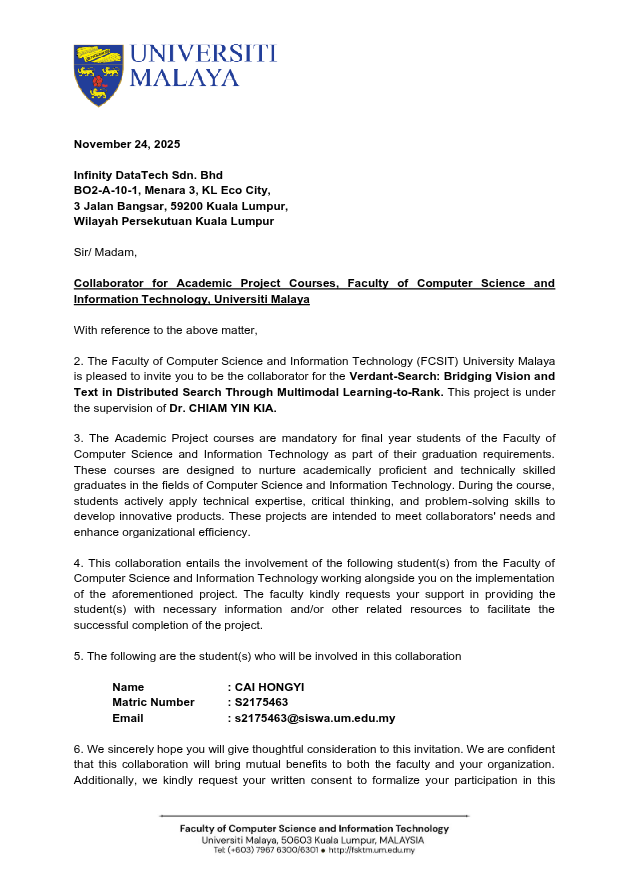
\includegraphics[width=0.30\textwidth]{collab1.png} &
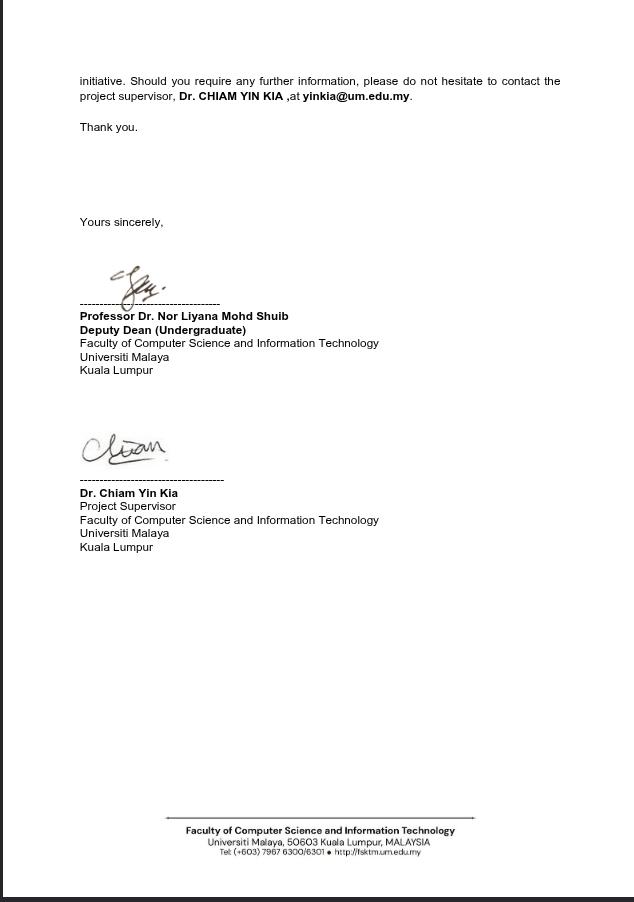
\includegraphics[width=0.30\textwidth]{collab2.png} &
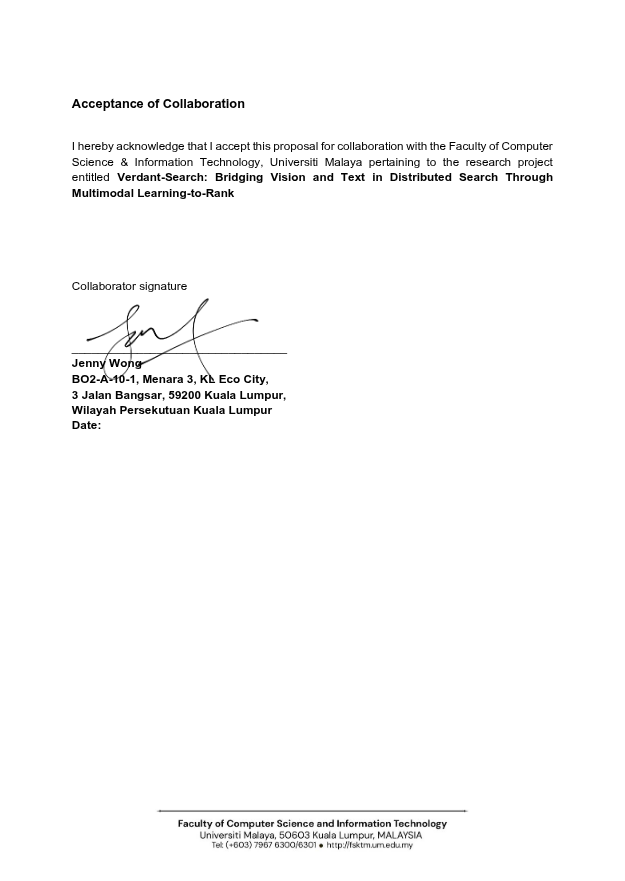
\includegraphics[width=0.30\textwidth]{collab3.png} \\
Page 1 & Page 2 & Page 3
\end{tabular}
\caption{Stakeholder Collaboration Agreement Letter from Infinity Datatech}
\label{fig:collaboration_letter}
\end{figure}

\subsection{Initial Requirements Gathering Sessions}

The initial requirements gathering process included structured meetings with various stakeholders to understand the current search pain points and identify opportunities for improvement. Key activities included:

\begin{itemize}
    \item Mapping the current information retrieval workflow across fragmented systems
    \item Identifying the 7 average context switches per search session
    \item Documenting the diverse types of information retrieval queries encountered by engineering teams, including technical how-to questions (e.g., "How to configure OAuth2 authentication in our API gateway?"), troubleshooting queries (e.g., "Why is the Redis cluster experiencing high memory usage?"), and policy-related questions (e.g., "What is the data retention policy for user analytics logs?")
    \item Understanding the 40\% of queries requiring visual evidence
\end{itemize}


\subsection{System Architecture Review Meetings}

The team conducted architecture review sessions to validate the proposed system design. Key discussion points included:

\begin{itemize}
    \item \textbf{Backend Pipeline}: The backend architecture comprises distributed web crawling with dedicated text and image extraction modules, dual indexing strategy utilizing inverted indices for BM25 keyword-based retrieval alongside Hierarchical Navigable Small World (HNSW) graphs for CLIP embedding-based semantic search, compressed document storage with incremental update capabilities, and a two-stage ranking pipeline that performs fast initial retrieval followed by multimodal learning-to-rank (LTR) reranking to optimize result relevance.
    \item \textbf{Frontend Interface}: The user interface features a dual-panel design that simultaneously displays a ranked document list alongside an AI-powered conversational chat interface, enabling conversational query refinement through natural language interactions, providing real-time result updates as users explore search results, and implementing a closed-loop feedback system where user follow-up questions automatically trigger query rewriting and initiate new retrieval cycles to progressively refine search outcomes.
\end{itemize}

\subsection{Product Review Meeting}

In-person product review meetings were conducted at Infinity Datatech's office to demonstrate the search engine prototype and gather direct feedback from stakeholders. These face-to-face sessions were crucial for validating the implemented features against the initial requirements and identifying areas for improvement.

During these review sessions, the development team presented live demonstrations of the multimodal search capabilities, including:

\begin{itemize}
    \item \textbf{Search Interface Walkthrough}: Demonstrating the dual-panel UI with real-time search results and AI-powered chat interface
    \item \textbf{Multimodal Retrieval Testing}: Showcasing the system's ability to retrieve documents based on both textual queries (e.g., searching for "microservices deployment architecture") and visual content such as architectural diagrams, performance charts, data flow graphs, and technical screenshots embedded within documentation
    \item \textbf{Performance Metrics Review}: Presenting comprehensive performance analytics including sub-second query latency measurements (p50, p95, p99 percentiles), document indexing throughput rates, and retrieval quality metrics such as Normalized Discounted Cumulative Gain (NDCG) and Mean Reciprocal Rank (MRR) evaluated against ground-truth relevance judgments
    \item \textbf{User Experience Feedback}: Gathering stakeholder input on interface usability, result relevance, and feature priorities for subsequent iterations
\end{itemize}

As shown in Figure~\ref{fig:product_review_meeting}, these collaborative sessions fostered direct communication between the developer and industry stakeholders, enabling immediate clarification of requirements and rapid iteration on the product design. The hands-on review approach proved invaluable for ensuring that the technical implementation aligned with the practical needs of end users within the organization.

\begin{figure}[H]
\centering
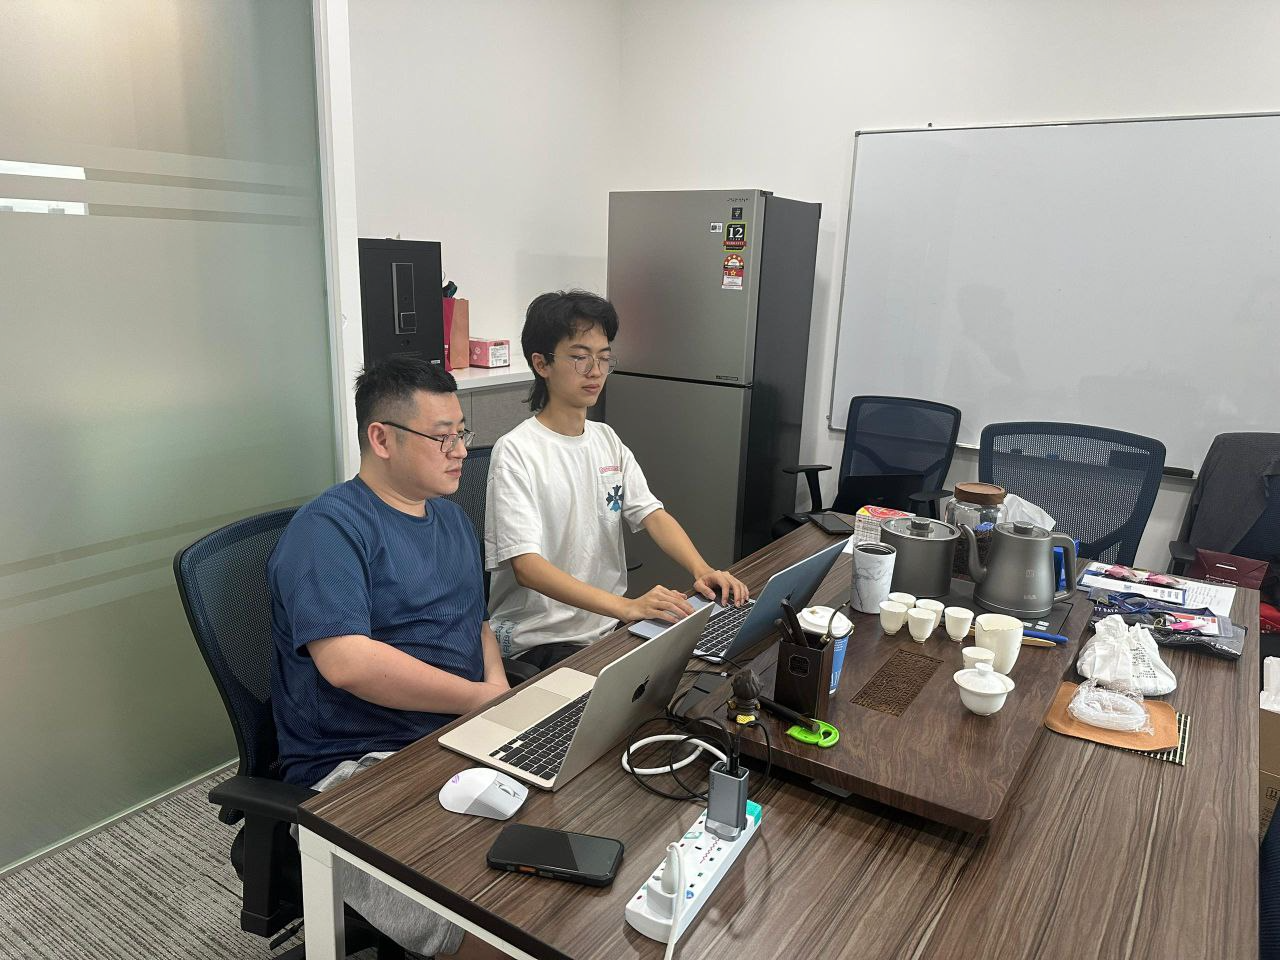
\includegraphics[width=0.75\textwidth]{physicalpic.png}
\caption{In-person Product Review Meeting with Infinity Datatech stakeholders discussing search engine features and user experience}
\label{fig:product_review_meeting}
\end{figure}

\subsection{Meeting Appointments}

Regular sync-up meetings were held with the industry collaborators throughout the development cycle. These meetings ensured continuous alignment between the search engine development and Infinity Datatech's evolving requirements. The project utilized Lark (Feishu) calendar for scheduling and coordinating meetings with stakeholders, including weekly progress reviews, technical discussions, and requirement clarification sessions.

As shown in Figure~\ref{fig:meeting_appointments}, the team maintained a structured meeting schedule throughout December 2025, with dedicated time slots for FYP discussions and milestone reviews. This systematic approach to stakeholder communication ensured that development priorities remained aligned with business needs and that technical challenges were addressed promptly through collaborative problem-solving.

\begin{figure}[H]
\centering
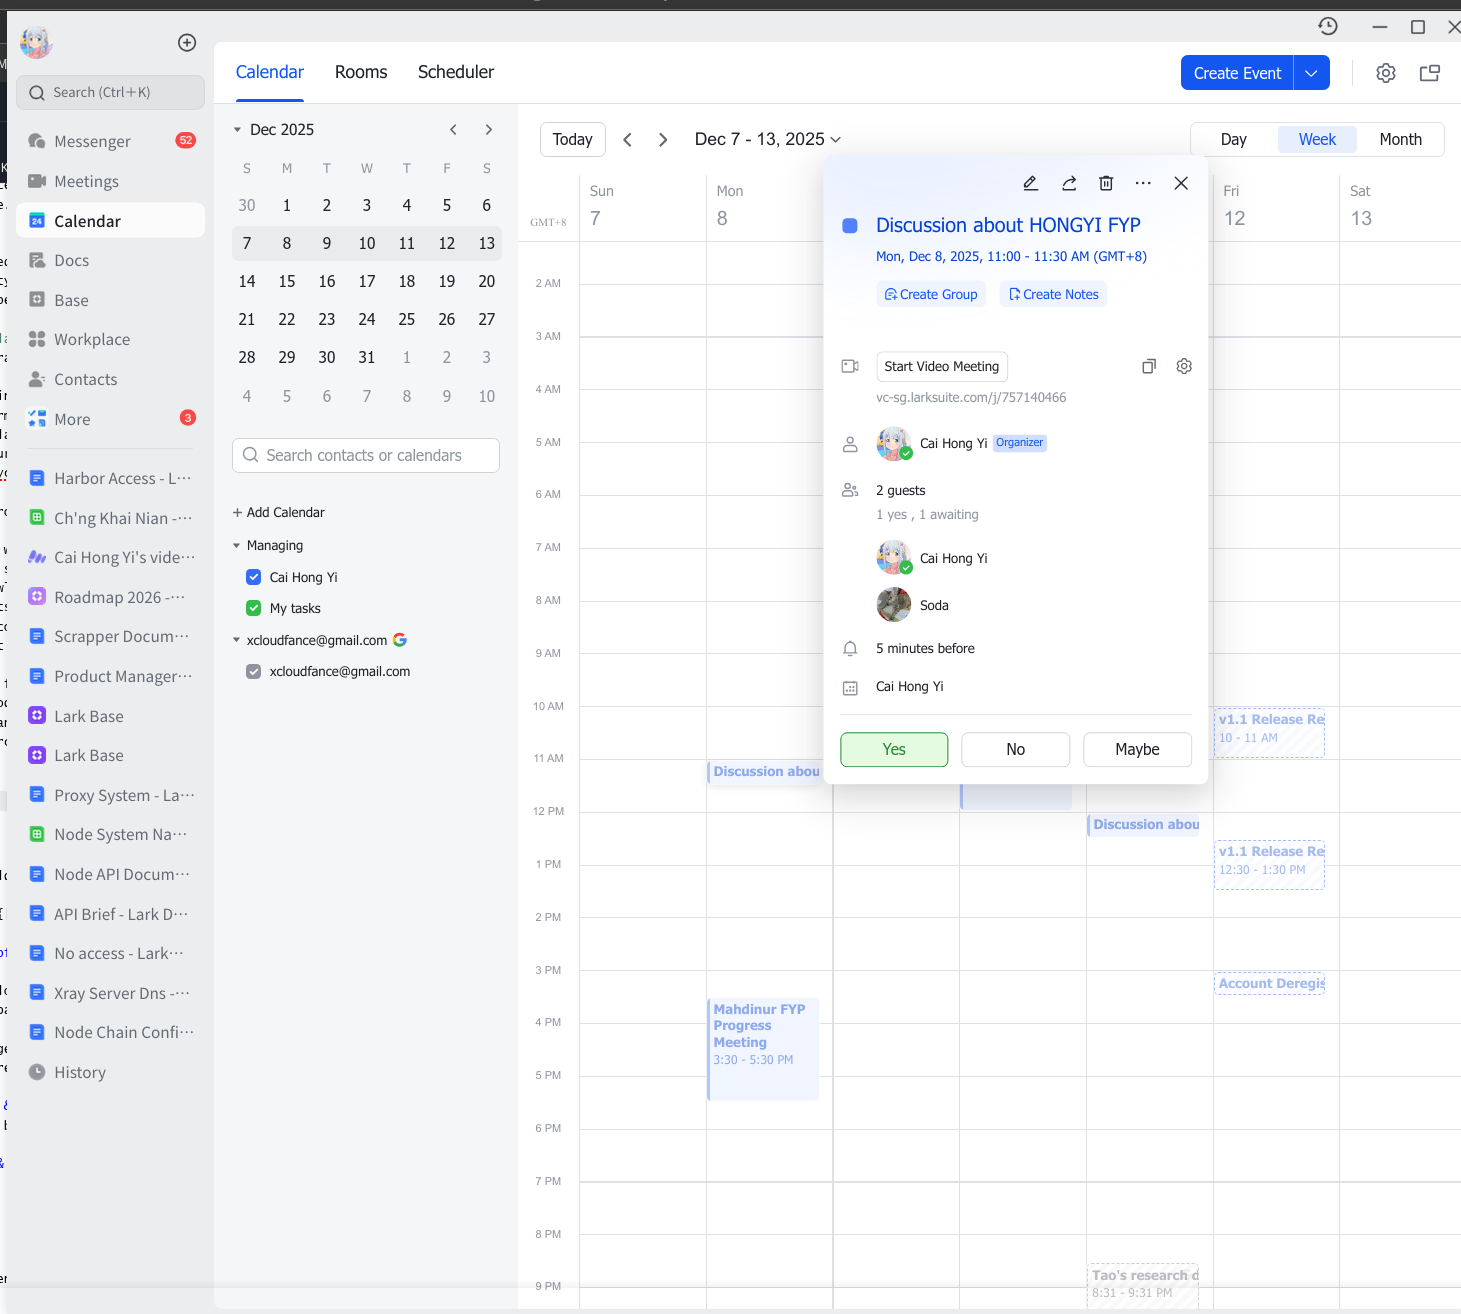
\includegraphics[width=0.85\textwidth]{FYPschedulescreenshot.png}
\caption{Meeting Appointments Schedule in Lark Calendar showing regular FYP sync-up sessions}
\label{fig:meeting_appointments}
\end{figure}

% ============================================================
% CHAPTER 5: SYSTEM ANALYSIS AND DESIGN
% ============================================================
\chapter{System Analysis and Design}
This chapter details the analysis and design of the Verdant Search multimodal enterprise search engine, outlining its architecture, functional and non-functional requirements, and key design aspects based on Infinity Datatech's specific needs for optimizing enterprise knowledge management and document retrieval.

\section{Key System Modules}
The Verdant Search platform consists of five core modules, each providing distinct functionality while working together as an integrated system to address Infinity Datatech's multimodal search and retrieval needs.

\subsection{Module 1: User Management System}
This module handles authentication, authorization, and user profile management for the entire platform. It manages user login, registration, and session handling using secure authentication mechanisms including SSO integration with enterprise identity providers (LDAP, Okta, Azure AD). The role-based access control system assigns permissions ensuring users can only access documents they are authorized to view. The system maintains comprehensive audit trails of all access events, authentication attempts, and permission changes. Users can manage their profiles with configurable preferences including display settings, notification preferences, and search history management. The module also provides session management with automatic timeout and token validation to ensure secure access throughout the platform.

\subsection{Module 2: Search and Retrieval System}
This module forms the core functionality of Verdant Search, implementing hybrid search capabilities that combine BM25 keyword-based retrieval with HNSW vector search. The system accepts user queries through a text input interface, performing query normalization and sanitization. For keyword search, it utilizes an inverted index with BM25 scoring to enable fast lexical matching. Simultaneously, the vector search component encodes queries using Sentence-BERT embeddings and performs approximate nearest neighbor search using HNSW indices over CLIP-embedded documents and images. The system implements Reciprocal Rank Fusion (RRF) to combine scores from both retrieval methods, producing a unified ranked list. Advanced multimodal reranking is then applied to top candidates using BLIP-2 for cross-modal relevance scoring. The module supports metadata filtering, conversational search refinement, and maintains conversation context across multiple search turns through intelligent query rewriting.

\subsection{Module 3: Data Ingestion and Indexing System}
This module manages the complete data ingestion pipeline from multiple enterprise sources. It implements distributed crawling capabilities using Kafka for job coordination and task distribution across worker nodes. The system supports crawling from diverse sources including Confluence spaces (via REST API), Google Drive (via Drive API), Git repositories (via Git protocol), and local network shares (via SMB/NFS). Each crawler respects rate limits and implements exponential backoff for failed operations. Once documents are retrieved, the extraction subsystem processes them to extract both textual content and embedded images, with OCR support for scanned PDFs. The chunking component segments documents into semantic units using multiple strategies (heading structure, paragraph boundaries, fixed token counts) while maintaining overlap for context preservation. Finally, the indexing subsystem builds both inverted indices for BM25 using Pyserini and HNSW vector indices using FAISS, generating dense embeddings with Sentence-BERT for text and CLIP for images. The module supports both scheduled batch updates and real-time synchronization via webhooks.

\subsection{Module 4: Analytics and Monitoring System}
This module provides comprehensive observability into system performance and search quality. It collects and visualizes system metrics including query latency (p50, p95, p99), indexing throughput, and resource utilization using Prometheus and Grafana. The analytics engine tracks search quality metrics such as click-through rates, query success rates, and user engagement patterns. It monitors the health of all distributed components including crawler workers, indexing jobs, and retrieval services. The module generates alerts for anomalies in system behavior, performance degradation, or service failures, enabling proactive issue resolution. It also provides administrators with dashboards for monitoring indexing progress, query volume trends, and resource consumption across the platform.

\subsection{Module 5: RAG Generation System}
This module implements the retrieval-augmented generation capabilities that enable conversational interaction with search results. Upon receiving a user query, the system retrieves relevant document chunks using the Search and Retrieval module, then injects this context into carefully structured prompts for the LLM. The generation engine uses SGLang for efficient LLM serving, generating answers grounded exclusively in retrieved content to prevent hallucination. Answers are streamed to the user in real-time using server-sent events, formatted with markdown for readability. The system automatically adds inline citations linking to source documents with page numbers, enabling users to verify claims. The module maintains conversation history, detecting follow-up questions and rewriting them into standalone queries using the LLM with full conversational context. This creates a closed-loop system where LLM insights trigger new retrieval cycles, progressively refining search results. The module implements entailment checking to validate answer grounding and clearly indicates knowledge base limitations when queries cannot be answered from available documents.

\clearpage

\section{Hierarchical Task Analysis}

The Hierarchical Task Analysis (HTA) diagram shown in Figure \ref{fig:hta} illustrates the complete functional structure of the Verdant Search system. The system is organized into five primary modules: User Management, Search and Retrieval, Data Ingestion and Indexing, Analytics and Monitoring, and RAG Generation. Each module represents a distinct functional area that supports the overall system's purpose of providing comprehensive multimodal search, intelligent ranking, and conversational question answering capabilities for enterprise knowledge bases. The hierarchical breakdown shows how these primary tasks decompose into specific subtasks and operations, creating a clear visualization of the system's scope and organization. This task decomposition provides the foundation for the use cases and activity diagrams presented in subsequent sections.

\begin{figure}[H]
    \centering
    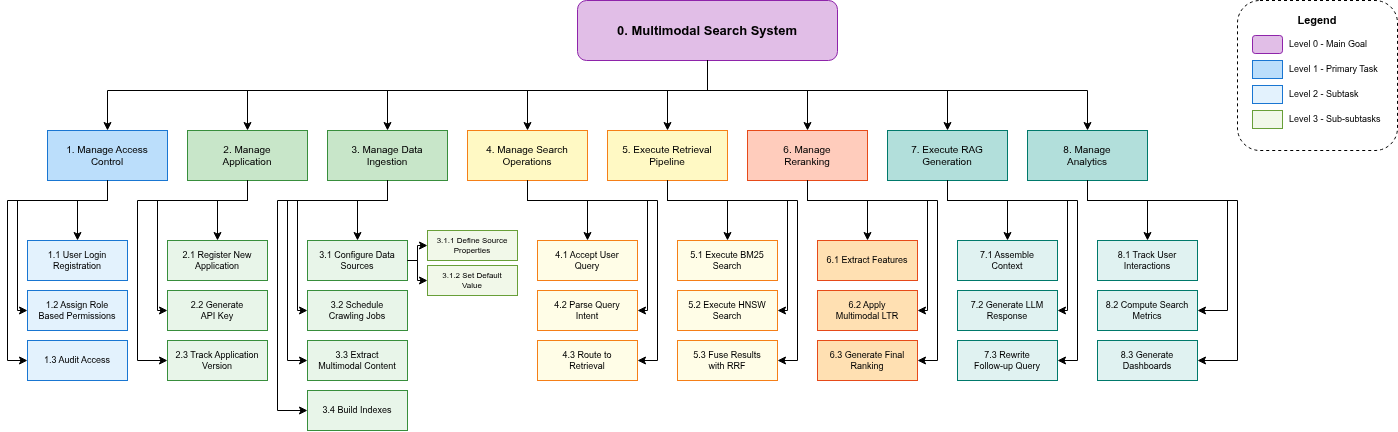
\includegraphics[width=\textwidth]{HTA.drawio.png}
    \caption{Hierarchical Task Analysis of Verdant Search System}
    \label{fig:hta}
\end{figure}
\clearpage


\section{Use Case Diagram}
\begin{figure}[H]
    \centering
    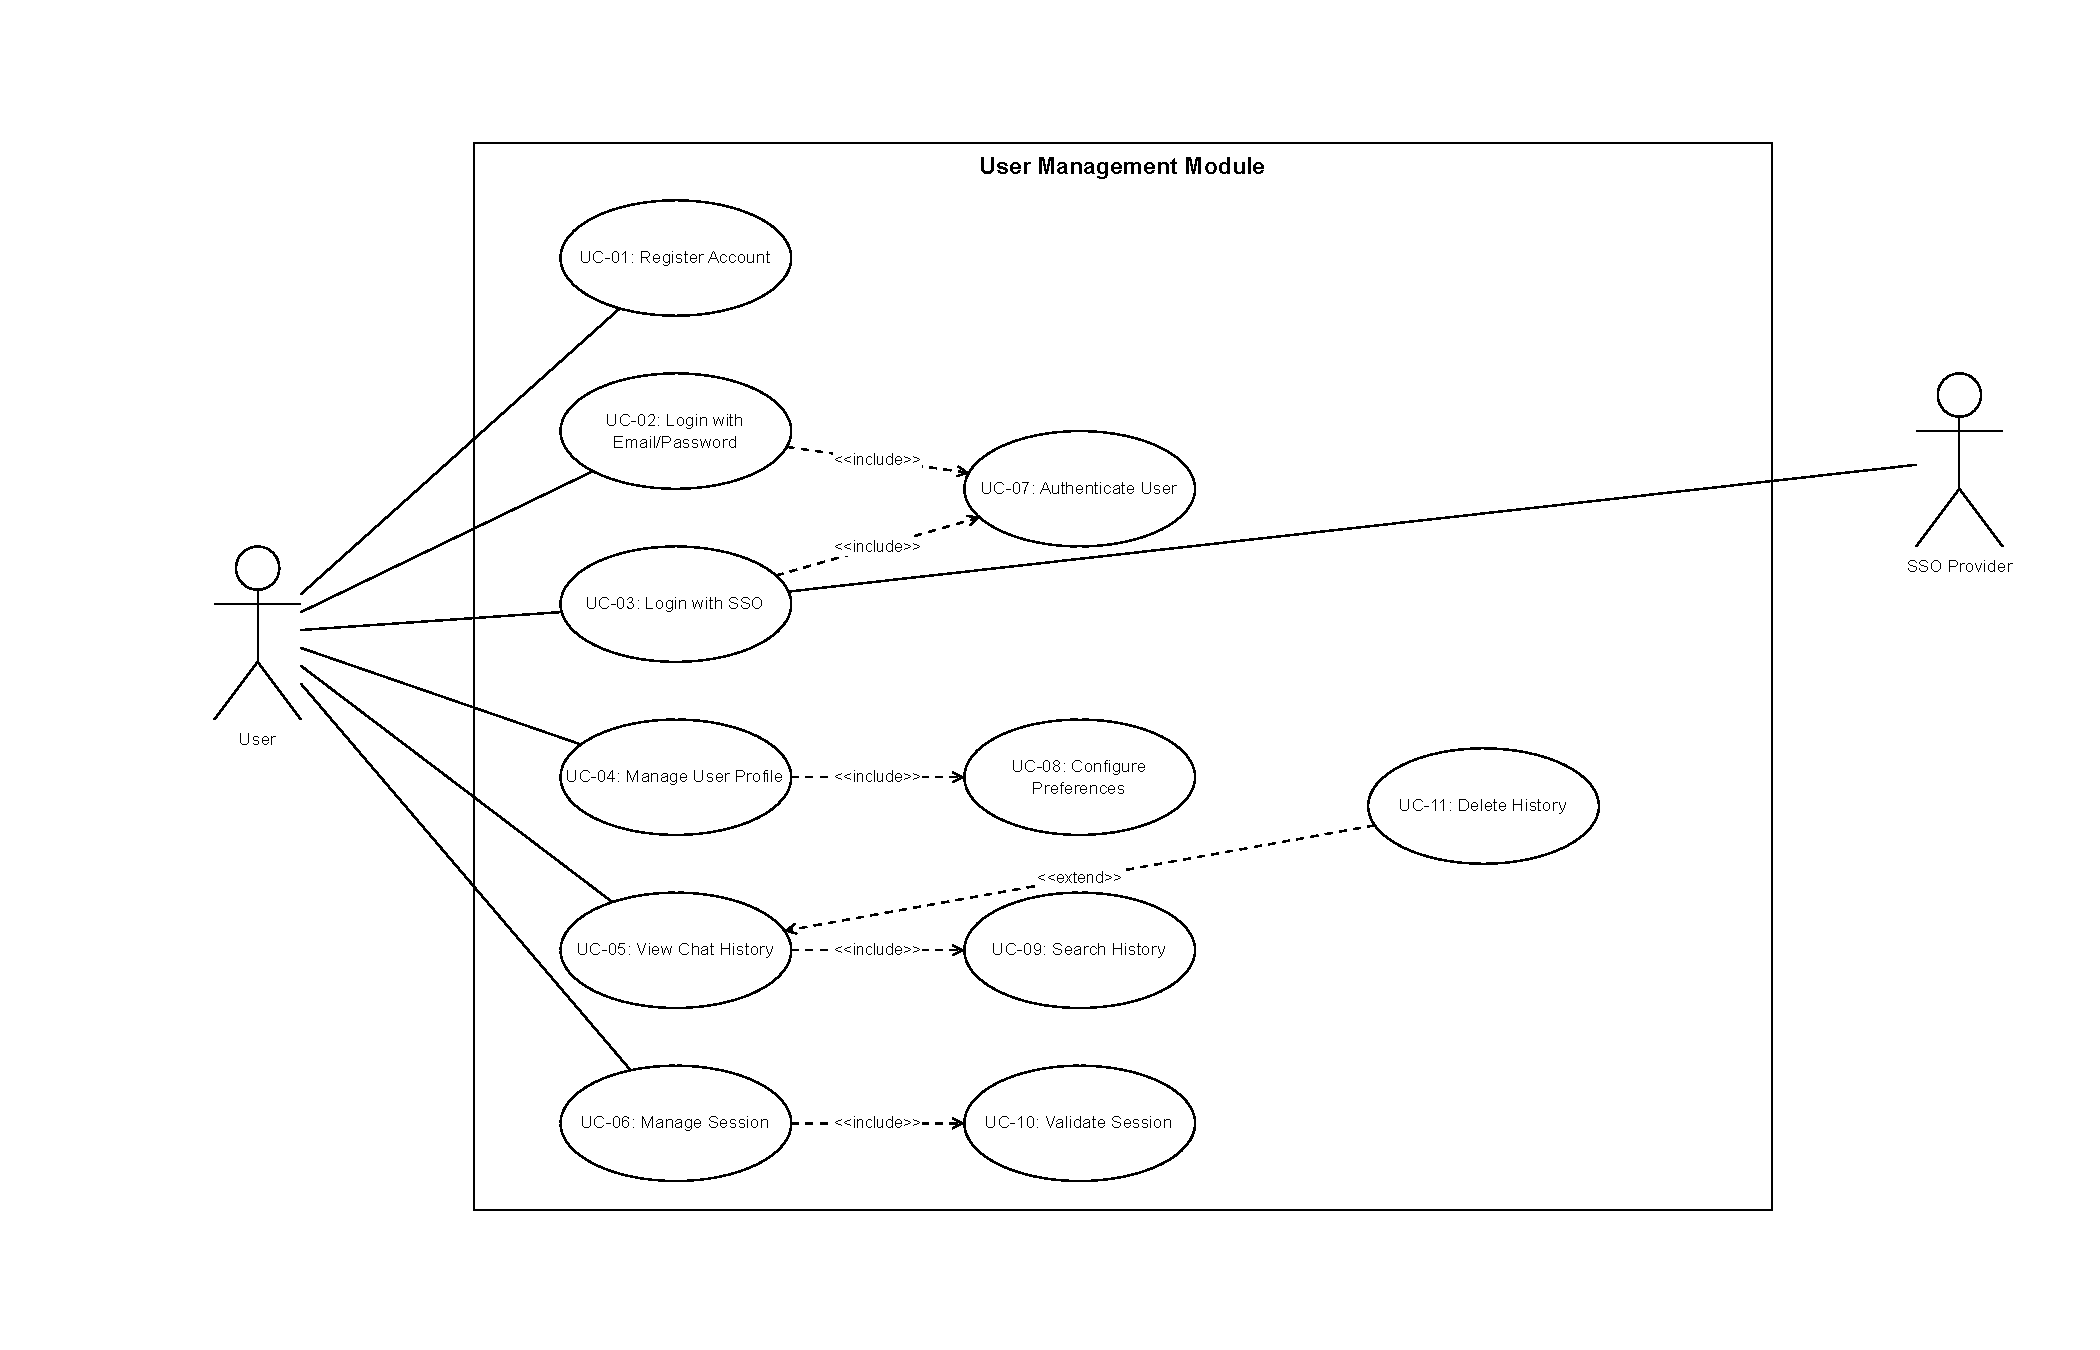
\includegraphics[width=0.95\textwidth,height=0.85\textheight,keepaspectratio]{updated_uc1.drawio.pdf}
    \caption{Use Case Diagram of Verdant Search System - User Management Module}
    \label{fig:usecase1}
\end{figure}

\noindent The Use Case Diagram illustrated above presents the User Management module of the Verdant Search system. This diagram shows how different actors (User, Administrator, System) interact with authentication, authorization, and profile management functionalities through various use cases.
\clearpage

\begin{figure}[H]
    \centering
    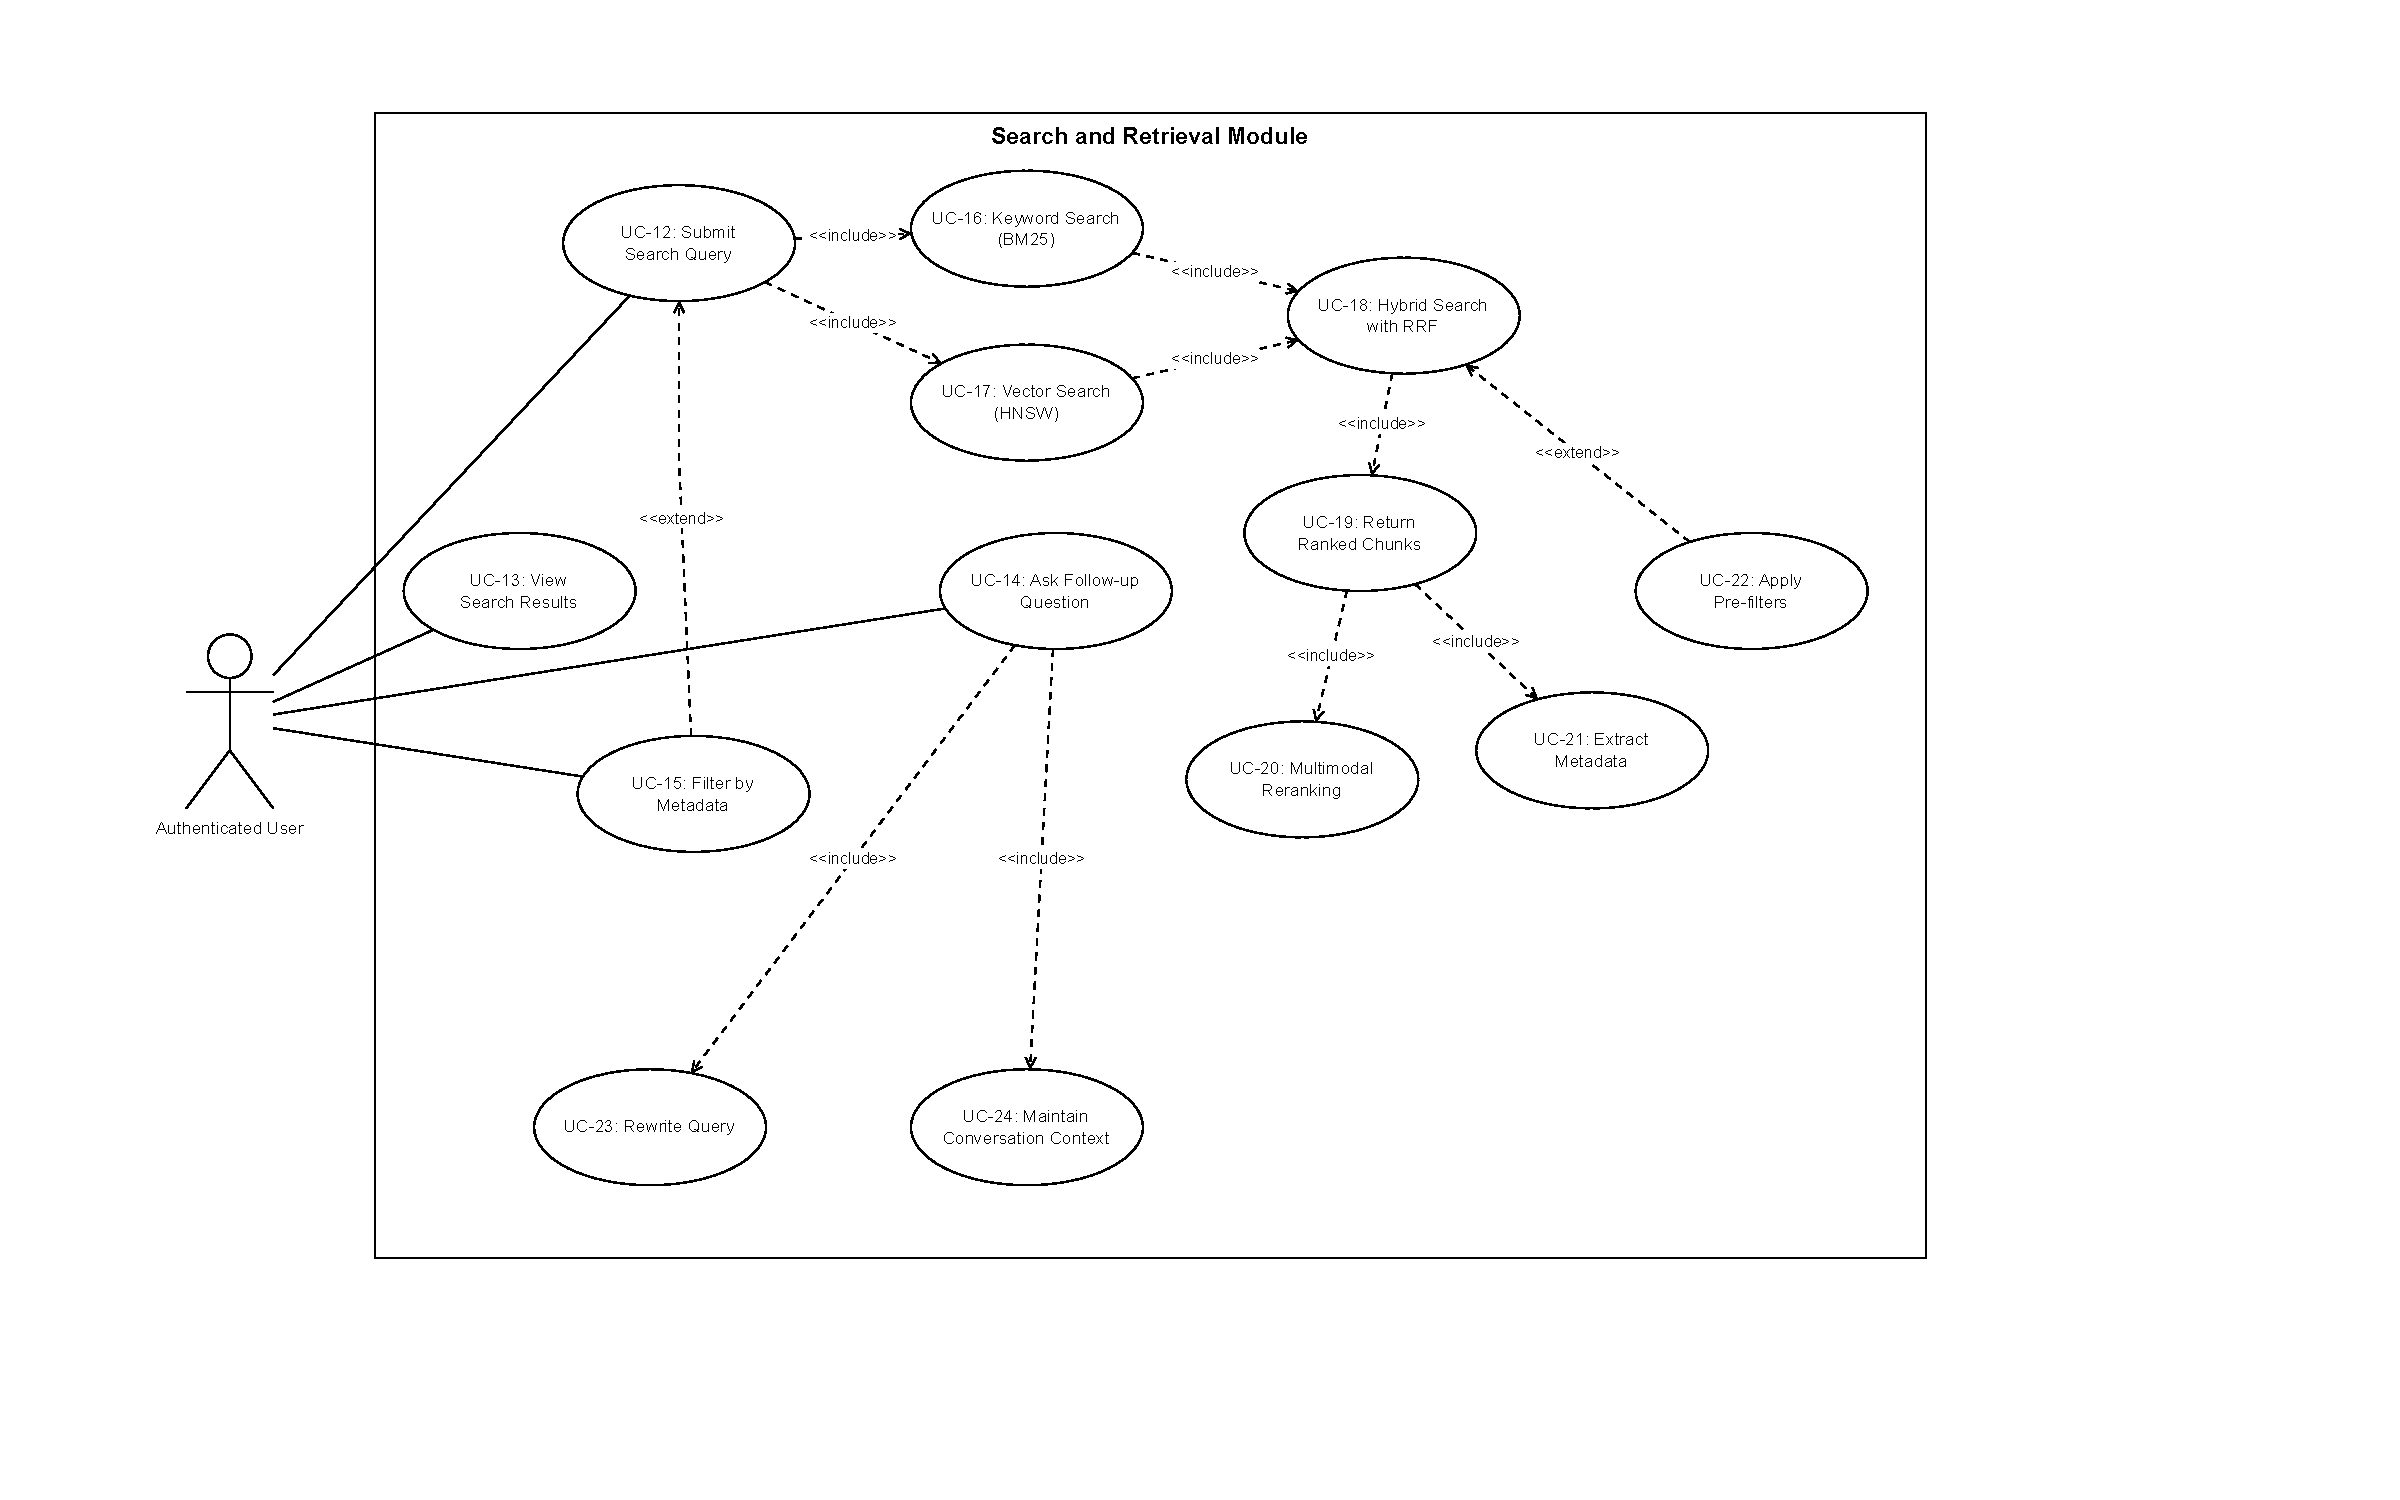
\includegraphics[width=0.95\textwidth,height=0.85\textheight,keepaspectratio]{updated_uc2.drawio.pdf}
    \caption{Use Case Diagram of Verdant Search System - Search and Retrieval Module}
    \label{fig:usecase2}
\end{figure}

\noindent This diagram presents the Search and Retrieval module, illustrating how users interact with the hybrid search system combining BM25 keyword search and HNSW vector search, along with multimodal reranking and conversational refinement capabilities.
\clearpage

\begin{figure}[H]
    \centering
    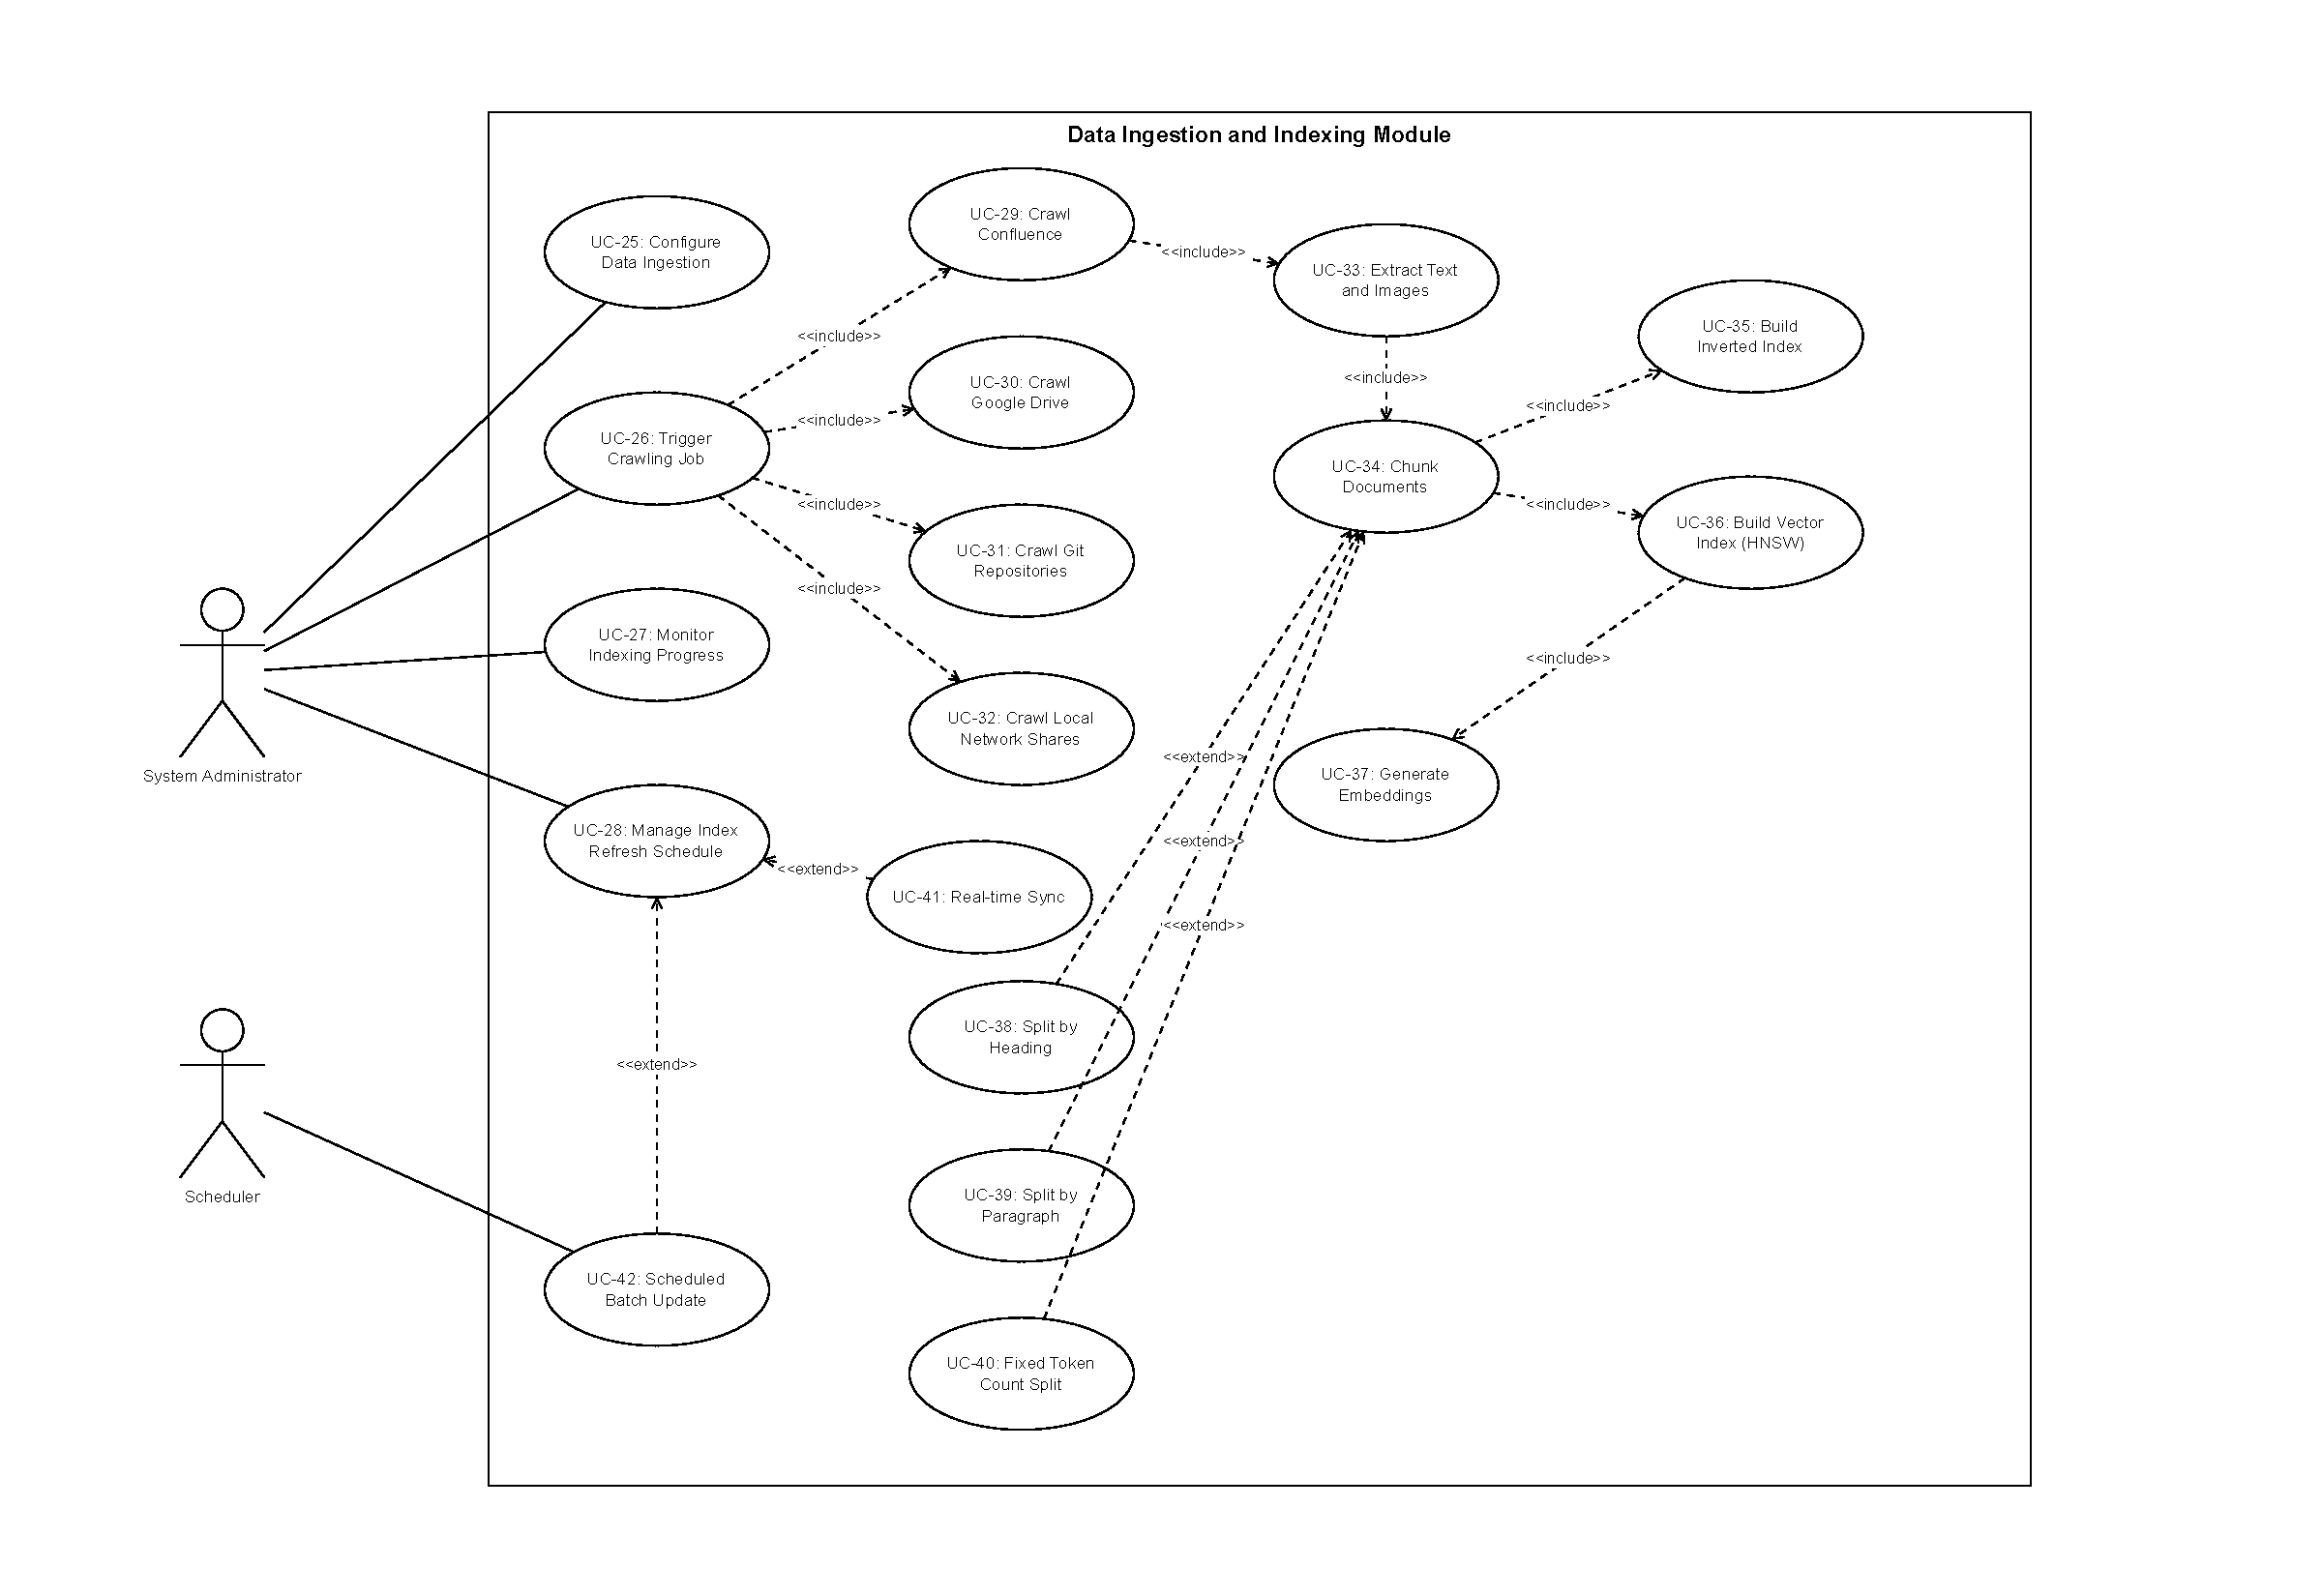
\includegraphics[width=0.95\textwidth,height=0.85\textheight,keepaspectratio]{updated_uc3.drawio.pdf}
    \caption{Use Case Diagram of Verdant Search System - Data Ingestion Module}
    \label{fig:usecase3}
\end{figure}

\noindent This diagram shows the Data Ingestion and Indexing module, depicting how administrators configure and manage distributed crawling across multiple enterprise data sources (Confluence, Google Drive, Git, network shares), and how the system processes, chunks, and indexes documents for efficient retrieval.
\clearpage

\begin{figure}[H]
    \centering
    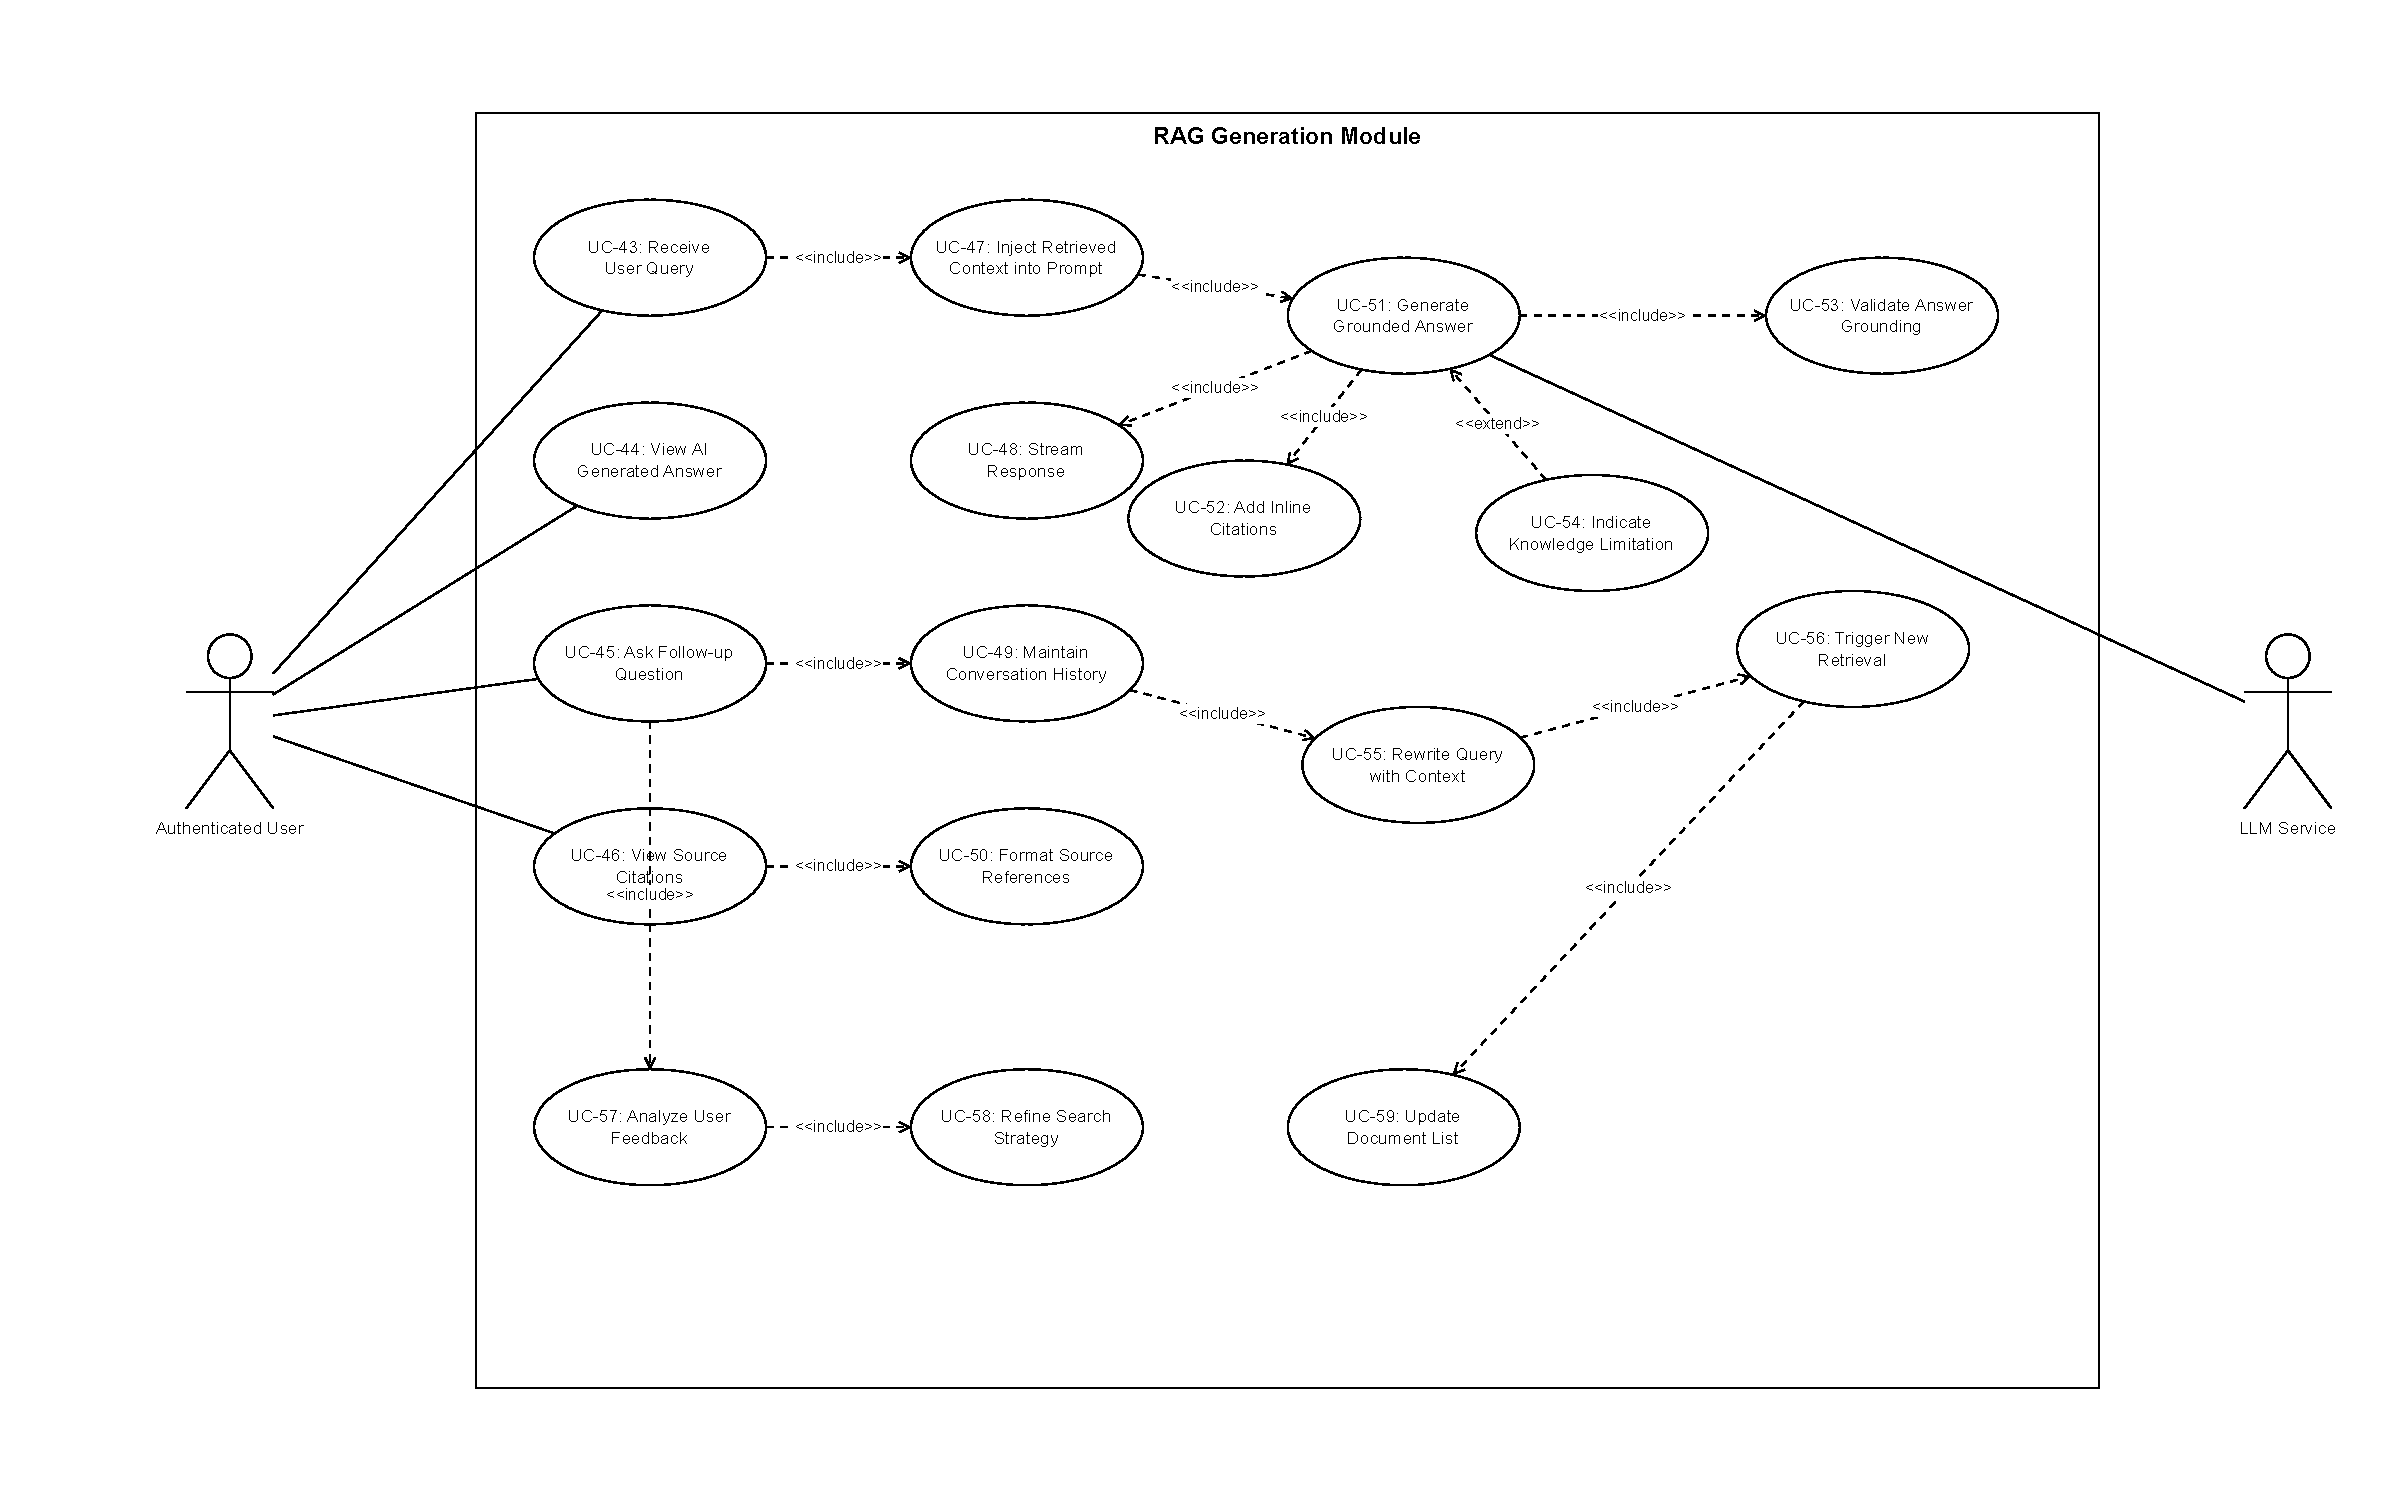
\includegraphics[width=0.95\textwidth,height=0.85\textheight,keepaspectratio]{updated_uc4.drawio.pdf}
    \caption{Use Case Diagram of Verdant Search System - RAG Generation Module}
    \label{fig:usecase4}
\end{figure}

\noindent This diagram illustrates the RAG Generation module, showing how the system generates AI-powered answers grounded in retrieved context, maintains conversational history, rewrites follow-up queries, and provides citations to source documents.
\clearpage


\section{Use Case Tables}

\begin{longtable}{|>{\raggedright\arraybackslash}p{0.08\textwidth}|>{\raggedright\arraybackslash}p{0.22\textwidth}|>{\raggedright\arraybackslash}p{0.62\textwidth}|}
\hline
\textbf{UC No.} & \textbf{Use Case Name} & \textbf{Functional Requirements (FRs)} \\
\hline
\endfirsthead

\hline
\textbf{UC No.} & \textbf{Use Case Name} & \textbf{Functional Requirements (FRs)} \\
\hline
\endhead

\hline \multicolumn{3}{r|}{{Continued on next page}} \\
\hline
\endfoot

\hline
\endlastfoot

% --- Module 1: User Management System ---
UC-1 & User Registration &
\begin{frequirements}
\item \textbf{FR-1.1:} The system shall allow a new user to register for an account by providing email and password.
\item \textbf{FR-1.2:} The system shall validate email format and enforce password strength requirements.
\item \textbf{FR-1.3:} The system shall send verification email upon successful registration.
\end{frequirements} \\
\hline

UC-2 & User Login via SSO &
\begin{frequirements}
\item \textbf{FR-1.4:} The system shall authenticate users via LDAP, Okta, or Azure AD SSO providers.
\item \textbf{FR-1.5:} The system shall support OAuth2 and SAML authentication protocols.
\item \textbf{FR-1.6:} The system shall generate JWT tokens for authenticated sessions.
\end{frequirements} \\
\hline

UC-3 & User Login via Email/Password &
\begin{frequirements}
\item \textbf{FR-1.7:} The system shall authenticate registered users based on email and password credentials.
\item \textbf{FR-1.8:} The system shall maintain user sessions after successful authentication.
\item \textbf{FR-1.9:} The system shall implement session timeout after 24 hours of inactivity.
\end{frequirements} \\
\hline

UC-4 & Manage User Profile &
\begin{frequirements}
\item \textbf{FR-1.10:} Users shall be able to update their display name, avatar, and notification preferences.
\item \textbf{FR-1.11:} Users shall be able to configure language and search result preferences.
\item \textbf{FR-1.12:} The system shall validate and store profile changes securely.
\end{frequirements} \\
\hline

UC-5 & View Chat History &
\begin{frequirements}
\item \textbf{FR-1.13:} The system shall display user chat history with timestamps and conversation summaries.
\item \textbf{FR-1.14:} Users shall be able to search within their chat history by keywords or date range.
\item \textbf{FR-1.15:} Users shall be able to export chat history in JSON or markdown format.
\end{frequirements} \\
\hline

UC-6 & Manage Session &
\begin{frequirements}
\item \textbf{FR-1.16:} The system shall validate session tokens on each authenticated request.
\item \textbf{FR-1.17:} The system shall automatically invalidate sessions after 24 hours.
\item \textbf{FR-1.18:} Users shall be able to manually log out to terminate their session.
\end{frequirements} \\
\hline

UC-7 & Authenticate User &
\begin{frequirements}
\item \textbf{FR-1.19:} The system shall verify user credentials against stored hashed passwords.
\item \textbf{FR-1.20:} The system shall log all authentication attempts with timestamps and outcomes.
\item \textbf{FR-1.21:} The system shall enforce rate limiting on failed authentication attempts.
\end{frequirements} \\
\hline

UC-8 & Configure User Settings &
\begin{frequirements}
\item \textbf{FR-1.22:} Users shall be able to set preferred search result display format.
\item \textbf{FR-1.23:} Users shall be able to configure notification preferences for search alerts.
\item \textbf{FR-1.24:} The system shall persist user settings across sessions.
\end{frequirements} \\
\hline

UC-9 & Search Chat History &
\begin{frequirements}
\item \textbf{FR-1.25:} The system shall support full-text search across user chat history.
\item \textbf{FR-1.26:} Search results shall highlight matching keywords in chat messages.
\item \textbf{FR-1.27:} The system shall rank search results by relevance and recency.
\end{frequirements} \\
\hline

UC-10 & Validate Session Token &
\begin{frequirements}
\item \textbf{FR-1.28:} The system shall verify JWT token signature and expiration on each request.
\item \textbf{FR-1.29:} The system shall reject expired or malformed tokens.
\item \textbf{FR-1.30:} The system shall return appropriate HTTP status codes for authentication failures.
\end{frequirements} \\
\hline

UC-11 & Delete Chat Entry &
\begin{frequirements}
\item \textbf{FR-1.31:} Users shall be able to delete individual chat conversations.
\item \textbf{FR-1.32:} Users shall be able to perform bulk deletion of chat history.
\item \textbf{FR-1.33:} The system shall prompt for confirmation before permanent deletion.
\end{frequirements} \\
\hline

% --- Module 2: Search and Retrieval System ---
UC-12 & Submit Search Query &
\begin{frequirements}
\item \textbf{FR-2.1:} The system shall accept search queries via text input interface.
\item \textbf{FR-2.2:} The system shall sanitize and normalize query text to prevent injection attacks.
\item \textbf{FR-2.3:} The system shall support query expansion with synonym detection.
\end{frequirements} \\
\hline

UC-13 & Display Search Results &
\begin{frequirements}
\item \textbf{FR-2.4:} The system shall present search results as a ranked list of documents.
\item \textbf{FR-2.5:} Each result shall display document title, snippet, and relevance score.
\item \textbf{FR-2.6:} The system shall highlight query keywords in document snippets.
\end{frequirements} \\
\hline

UC-14 & Ask Follow-up Question &
\begin{frequirements}
\item \textbf{FR-2.7:} Users shall be able to ask follow-up questions within the same conversation.
\item \textbf{FR-2.8:} The system shall detect whether input is a follow-up or new query.
\item \textbf{FR-2.9:} The system shall maintain conversation context across multiple turns.
\end{frequirements} \\
\hline

UC-15 & Filter Results by Metadata &
\begin{frequirements}
\item \textbf{FR-2.10:} Users shall be able to filter results by document type, date range, and source.
\item \textbf{FR-2.11:} The system shall apply filters before ranking to reduce computational cost.
\item \textbf{FR-2.12:} The system shall display active filters in the user interface.
\end{frequirements} \\
\hline

UC-16 & Perform Keyword Search &
\begin{frequirements}
\item \textbf{FR-2.13:} The system shall build and maintain an inverted index for BM25 retrieval.
\item \textbf{FR-2.14:} The system shall score documents using BM25 with tunable k1 and b parameters.
\item \textbf{FR-2.15:} The system shall return top K candidates from keyword search.
\end{frequirements} \\
\hline

UC-17 & Perform Vector Search &
\begin{frequirements}
\item \textbf{FR-2.16:} The system shall encode queries into dense vectors using Sentence-BERT.
\item \textbf{FR-2.17:} The system shall build HNSW index for approximate nearest neighbor search.
\item \textbf{FR-2.18:} The system shall return top K candidates from vector search with cosine similarity scores.
\end{frequirements} \\
\hline

UC-18 & Perform Hybrid Search &
\begin{frequirements}
\item \textbf{FR-2.19:} The system shall combine BM25 and vector search results using Reciprocal Rank Fusion.
\item \textbf{FR-2.20:} The system shall support weighted fusion with configurable alpha parameter.
\item \textbf{FR-2.21:} The system shall deduplicate results from both retrieval methods.
\end{frequirements} \\
\hline

UC-19 & Retrieve Context Chunks &
\begin{frequirements}
\item \textbf{FR-2.22:} The system shall return document chunks with surrounding context for RAG.
\item \textbf{FR-2.23:} Each chunk shall include metadata (filename, page number, timestamp).
\item \textbf{FR-2.24:} The system shall limit total context size to fit LLM context window.
\end{frequirements} \\
\hline

UC-20 & Apply Multimodal Reranking &
\begin{frequirements}
\item \textbf{FR-2.25:} The system shall apply multimodal reranking to top K candidates from hybrid search.
\item \textbf{FR-2.26:} The system shall use BLIP-2 vision-language model for cross-modal relevance scoring.
\item \textbf{FR-2.27:} The system shall reorder results based on multimodal relevance scores.
\end{frequirements} \\
\hline

UC-21 & Extract Chunk Metadata &
\begin{frequirements}
\item \textbf{FR-2.28:} The system shall attach source document filename to each chunk.
\item \textbf{FR-2.29:} The system shall include page number or section identifier for each chunk.
\item \textbf{FR-2.30:} The system shall record document creation and modification timestamps.
\end{frequirements} \\
\hline

UC-22 & Apply Pre-filtering &
\begin{frequirements}
\item \textbf{FR-2.31:} The system shall support filtering by document source before retrieval.
\item \textbf{FR-2.32:} The system shall enforce access control filters based on user permissions.
\item \textbf{FR-2.33:} The system shall apply date range filters if specified by user.
\end{frequirements} \\
\hline

UC-23 & Rewrite Follow-up Query &
\begin{frequirements}
\item \textbf{FR-2.34:} The system shall use LLM to rewrite follow-up questions into standalone queries.
\item \textbf{FR-2.35:} The system shall include conversation history as context for rewriting.
\item \textbf{FR-2.36:} The system shall trigger new retrieval cycle with rewritten query.
\end{frequirements} \\
\hline

UC-24 & Maintain Conversation Context &
\begin{frequirements}
\item \textbf{FR-2.37:} The system shall store conversation history in session memory.
\item \textbf{FR-2.38:} The system shall limit history to last 10 conversation turns to manage context size.
\item \textbf{FR-2.39:} The system shall provide conversation history to query rewriting module.
\end{frequirements} \\
\hline

% --- Module 3: Data Ingestion and Indexing System ---
UC-25 & Configure Data Sources &
\begin{frequirements}
\item \textbf{FR-3.1:} Administrators shall be able to configure Confluence, Google Drive, Git, and network share sources.
\item \textbf{FR-3.2:} The system shall validate source credentials and API permissions.
\item \textbf{FR-3.3:} The system shall encrypt and securely store source credentials.
\end{frequirements} \\
\hline

UC-26 & Trigger Distributed Crawling &
\begin{frequirements}
\item \textbf{FR-3.4:} Administrators shall be able to manually trigger crawling jobs.
\item \textbf{FR-3.5:} The system shall use Kafka for distributing crawl tasks across worker nodes.
\item \textbf{FR-3.6:} The system shall implement exponential backoff for failed crawl attempts.
\end{frequirements} \\
\hline

UC-27 & Monitor Indexing Progress &
\begin{frequirements}
\item \textbf{FR-3.7:} Administrators shall be able to view real-time indexing progress dashboard.
\item \textbf{FR-3.8:} The system shall display metrics including documents processed, errors, and throughput.
\item \textbf{FR-3.9:} The system shall provide estimated time to completion for indexing jobs.
\end{frequirements} \\
\hline

UC-28 & Manage Index Refresh &
\begin{frequirements}
\item \textbf{FR-3.10:} Administrators shall be able to schedule index refresh using cron expressions.
\item \textbf{FR-3.11:} The system shall support incremental index updates without full rebuilds.
\item \textbf{FR-3.12:} The system shall maintain index version history for rollback capability.
\end{frequirements} \\
\hline

UC-29 & Crawl Confluence &
\begin{frequirements}
\item \textbf{FR-3.13:} The system shall connect to Confluence instances via REST API.
\item \textbf{FR-3.14:} The system shall respect Confluence rate limits and implement pagination.
\item \textbf{FR-3.15:} The system shall extract page content, attachments, and comments.
\end{frequirements} \\
\hline

UC-30 & Crawl Google Drive &
\begin{frequirements}
\item \textbf{FR-3.16:} The system shall connect to Google Drive via Drive API with OAuth2 authentication.
\item \textbf{FR-3.17:} The system shall process Google Docs, Sheets, Slides, and PDF formats.
\item \textbf{FR-3.18:} The system shall extract sharing permissions and metadata from Drive files.
\end{frequirements} \\
\hline

UC-31 & Crawl Git Repositories &
\begin{frequirements}
\item \textbf{FR-3.19:} The system shall clone Git repositories using SSH or HTTPS protocols.
\item \textbf{FR-3.20:} The system shall index documentation files (Markdown, reStructuredText, text).
\item \textbf{FR-3.21:} The system shall associate commits with document versions for change tracking.
\end{frequirements} \\
\hline

UC-32 & Crawl Network Shares &
\begin{frequirements}
\item \textbf{FR-3.22:} The system shall access network shares via SMB and NFS protocols.
\item \textbf{FR-3.23:} The system shall authenticate using provided network credentials.
\item \textbf{FR-3.24:} The system shall recursively scan directory structures for documents.
\end{frequirements} \\
\hline

UC-33 & Extract Document Content &
\begin{frequirements}
\item \textbf{FR-3.25:} The system shall extract text from PDF, DOCX, PPTX, and HTML documents.
\item \textbf{FR-3.26:} The system shall extract embedded images with associated captions.
\item \textbf{FR-3.27:} The system shall apply OCR to scanned PDFs using Tesseract.
\end{frequirements} \\
\hline

UC-34 & Chunk Documents &
\begin{frequirements}
\item \textbf{FR-3.28:} The system shall segment documents into semantic chunks using heading structure.
\item \textbf{FR-3.29:} The system shall maintain 10\% chunk overlap to preserve context across boundaries.
\item \textbf{FR-3.30:} The system shall limit chunk size to 512 tokens for embedding model compatibility.
\end{frequirements} \\
\hline

UC-35 & Build Inverted Index &
\begin{frequirements}
\item \textbf{FR-3.31:} The system shall build inverted index using Pyserini framework.
\item \textbf{FR-3.32:} The system shall store term posting lists with term frequencies and positions.
\item \textbf{FR-3.33:} The system shall create index segments for incremental updates.
\end{frequirements} \\
\hline

UC-36 & Build HNSW Index &
\begin{frequirements}
\item \textbf{FR-3.34:} The system shall build HNSW graph index using FAISS library.
\item \textbf{FR-3.35:} The system shall configure M and ef\_construction parameters for index quality.
\item \textbf{FR-3.36:} The system shall persist HNSW index to disk for efficient loading.
\end{frequirements} \\
\hline

UC-37 & Generate Embeddings &
\begin{frequirements}
\item \textbf{FR-3.37:} The system shall generate text embeddings using Sentence-BERT model.
\item \textbf{FR-3.38:} The system shall generate image embeddings using CLIP vision encoder.
\item \textbf{FR-3.39:} The system shall batch embedding generation for GPU efficiency.
\end{frequirements} \\
\hline

UC-38 & Chunk by Heading &
\begin{frequirements}
\item \textbf{FR-3.40:} The system shall parse document structure to identify headings.
\item \textbf{FR-3.41:} The system shall create chunks at section boundaries defined by headings.
\item \textbf{FR-3.42:} The system shall preserve heading text as chunk metadata.
\end{frequirements} \\
\hline

UC-39 & Chunk by Paragraph &
\begin{frequirements}
\item \textbf{FR-3.43:} The system shall detect paragraph boundaries using newline patterns.
\item \textbf{FR-3.44:} The system shall merge small adjacent paragraphs to meet minimum chunk size.
\item \textbf{FR-3.45:} The system shall split large paragraphs at sentence boundaries.
\end{frequirements} \\
\hline

UC-40 & Chunk by Token Count &
\begin{frequirements}
\item \textbf{FR-3.46:} The system shall use tokenizer to measure chunk length in tokens.
\item \textbf{FR-3.47:} The system shall create fixed-size chunks of 512 tokens.
\item \textbf{FR-3.48:} The system shall implement sliding window with 10\% overlap.
\end{frequirements} \\
\hline

UC-41 & Sync with Webhooks &
\begin{frequirements}
\item \textbf{FR-3.49:} The system shall provide webhook endpoints for real-time update notifications.
\item \textbf{FR-3.50:} The system shall process webhook events to trigger incremental indexing.
\item \textbf{FR-3.51:} The system shall validate webhook signatures to prevent unauthorized updates.
\end{frequirements} \\
\hline

UC-42 & Schedule Batch Updates &
\begin{frequirements}
\item \textbf{FR-3.52:} Administrators shall be able to configure batch update schedules.
\item \textbf{FR-3.53:} The system shall execute scheduled crawls at specified intervals.
\item \textbf{FR-3.54:} The system shall send notification emails upon batch update completion.
\end{frequirements} \\
\hline

% --- Module 5: RAG Generation System ---
UC-43 & Receive User Query &
\begin{frequirements}
\item \textbf{FR-5.1:} The system shall accept user queries for RAG-based answer generation.
\item \textbf{FR-5.2:} The system shall validate query length and reject queries exceeding 1000 characters.
\item \textbf{FR-5.3:} The system shall queue queries during high load to prevent system overload.
\end{frequirements} \\
\hline

UC-44 & View Generated Answer &
\begin{frequirements}
\item \textbf{FR-5.4:} The system shall display AI-generated answers formatted with markdown.
\item \textbf{FR-5.5:} Answers shall include inline citations linking to source documents.
\item \textbf{FR-5.6:} The system shall highlight cited text when users click citation links.
\end{frequirements} \\
\hline

UC-45 & Ask Follow-up in RAG &
\begin{frequirements}
\item \textbf{FR-5.7:} Users shall be able to ask follow-up questions within RAG conversations.
\item \textbf{FR-5.8:} The system shall detect follow-up intent using conversation context.
\item \textbf{FR-5.9:} The system shall maintain both chat history and search result history.
\end{frequirements} \\
\hline

UC-46 & View Source Citations &
\begin{frequirements}
\item \textbf{FR-5.10:} Users shall be able to click citations to navigate to source documents.
\item \textbf{FR-5.11:} The system shall highlight cited passages in source document viewer.
\item \textbf{FR-5.12:} Citations shall display document title, page number, and relevance score.
\end{frequirements} \\
\hline

UC-47 & Inject Retrieved Context &
\begin{frequirements}
\item \textbf{FR-5.13:} The system shall inject top K retrieved chunks into LLM prompt.
\item \textbf{FR-5.14:} Context shall be formatted with clear delimiters and metadata.
\item \textbf{FR-5.15:} The system shall truncate context if it exceeds LLM context window limit.
\end{frequirements} \\
\hline

UC-48 & Stream LLM Response &
\begin{frequirements}
\item \textbf{FR-5.16:} The system shall stream LLM-generated text to users in real-time.
\item \textbf{FR-5.17:} The system shall use server-sent events (SSE) for streaming.
\item \textbf{FR-5.18:} The system shall handle connection interruptions gracefully.
\end{frequirements} \\
\hline

UC-49 & Maintain Conversation History &
\begin{frequirements}
\item \textbf{FR-5.19:} The system shall store conversation history in Redis cache.
\item \textbf{FR-5.20:} The system shall limit history to last 10 conversation turns.
\item \textbf{FR-5.21:} The system shall provide conversation history export functionality.
\end{frequirements} \\
\hline

UC-50 & Format Source References &
\begin{frequirements}
\item \textbf{FR-5.22:} The system shall format citations with document title, author, and timestamp.
\item \textbf{FR-5.23:} Citations shall use superscript numbering format [1], [2], etc.
\item \textbf{FR-5.24:} The system shall generate bibliography at end of answer listing all sources.
\end{frequirements} \\
\hline

UC-51 & Generate Grounded Answer &
\begin{frequirements}
\item \textbf{FR-5.25:} The LLM shall generate answers using only provided context chunks.
\item \textbf{FR-5.26:} The system shall instruct LLM to avoid hallucination in system prompt.
\item \textbf{FR-5.27:} The system shall mark uncertain responses with confidence qualifiers.
\end{frequirements} \\
\hline

UC-52 & Add Inline Citations &
\begin{frequirements}
\item \textbf{FR-5.28:} The system shall instruct LLM to include citation markers in generated text.
\item \textbf{FR-5.29:} Citations shall link to specific document chunks used for each claim.
\item \textbf{FR-5.30:} The system shall validate citation markers match provided sources.
\end{frequirements} \\
\hline

UC-53 & Validate Answer Grounding &
\begin{frequirements}
\item \textbf{FR-5.31:} The system shall use entailment model to verify answer claims against sources.
\item \textbf{FR-5.32:} The system shall flag unsupported claims for user review.
\item \textbf{FR-5.33:} The system shall log grounding validation scores for quality monitoring.
\end{frequirements} \\
\hline

UC-54 & Indicate Knowledge Gaps &
\begin{frequirements}
\item \textbf{FR-5.34:} The system shall detect when retrieved context is insufficient to answer query.
\item \textbf{FR-5.35:} The system shall display message indicating knowledge base limitations.
\item \textbf{FR-5.36:} The system shall suggest query refinements to improve retrieval.
\end{frequirements} \\
\hline

UC-55 & Rewrite Conversational Query &
\begin{frequirements}
\item \textbf{FR-5.37:} The system shall use LLM to rewrite follow-up questions into standalone queries.
\item \textbf{FR-5.38:} The system shall include full conversation history as rewriting context.
\item \textbf{FR-5.39:} The system shall preserve user intent while resolving coreferences.
\end{frequirements} \\
\hline

UC-56 & Trigger New Retrieval &
\begin{frequirements}
\item \textbf{FR-5.40:} The system shall automatically trigger search after query rewriting.
\item \textbf{FR-5.41:} The system shall use rewritten query for hybrid retrieval pipeline.
\item \textbf{FR-5.42:} The system shall cache rewritten queries to avoid duplicate processing.
\end{frequirements} \\
\hline

UC-57 & Analyze User Feedback &
\begin{frequirements}
\item \textbf{FR-5.43:} The system shall collect user ratings (thumbs up/down) for generated answers.
\item \textbf{FR-5.44:} The system shall store feedback with associated queries and contexts.
\item \textbf{FR-5.45:} The system shall analyze feedback patterns to identify quality issues.
\end{frequirements} \\
\hline

UC-58 & Refine Search Strategy &
\begin{frequirements}
\item \textbf{FR-5.46:} The system shall adjust retrieval parameters based on feedback analysis.
\item \textbf{FR-5.47:} The system shall increase diversity when users repeatedly refine queries.
\item \textbf{FR-5.48:} The system shall log strategy adjustments for performance evaluation.
\end{frequirements} \\
\hline

UC-59 & Update Document List &
\begin{frequirements}
\item \textbf{FR-5.49:} The system shall refresh displayed document list after new retrieval.
\item \textbf{FR-5.50:} Updated list shall maintain scroll position from previous view.
\item \textbf{FR-5.51:} The system shall highlight newly added documents from refined search.
\end{frequirements} \\
\hline

\end{longtable}

\section{Use Case Descriptions}

The following section provides detailed descriptions for selected representative use cases that demonstrate the core functionality of each system module.

\subsection*{Module 1: User Management System}

\subsubsection*{UC-1: User Registration}

\begin{table}[H]
\small
\begin{tabularx}{\textwidth}{|p{0.25\textwidth}|X|}
\hline
\textbf{Property} & \textbf{Details} \\
\hline
Use Case ID & UC-1 \\
\hline
Description & Allows new users to create an account on the Verdant Search platform \\
\hline
Priority & High \\
\hline  
Actor & User (prospective), System \\
\hline
Pre-condition & User does not have an existing account; System is operational \\
\hline
Post-condition & New user account is created; Verification email is sent; User can login after verification \\ 
\hline
Flow of Events & 1. User navigates to registration page \newline 2. System displays registration form \newline 3. User enters email and password (FR-1.1) \newline 4. System validates format and strength (FR-1.2) \newline 5. System creates account with hashed password \newline 6. System sends verification email (FR-1.3) \newline 7. System displays confirmation message \\
\hline
Exception Flow & - Email already exists: Error message displayed \newline - Password too weak: Validation error shown \newline - Email service fails: Account created but verification delayed \\
\hline
\end{tabularx}
\end{table}

\subsection*{Module 2: Search and Retrieval System}

\subsubsection*{UC-12: Submit Search Query}

\begin{table}[H]
\small
\begin{tabularx}{\textwidth}{|p{0.25\textwidth}|X|}
\hline
\textbf{Property} & \textbf{Details} \\
\hline
Use Case ID & UC-12 \\
\hline
Description & Allows users to initiate search by submitting text query, triggering hybrid retrieval pipeline \\
\hline
Priority & High \\
\hline
Actor & User, System \\
\hline
Pre-condition & User is authenticated; Search indices are built and available; Backend services operational \\
\hline
Post-condition & Query is processed and sanitized; Query logged for analytics; Hybrid retrieval triggered; User receives ranked results \\
\hline
Flow of Events & 1. User enters query in search box (FR-2.1) \newline 2. System validates query length \newline 3. System sanitizes query to prevent injection (FR-2.2) \newline 4. System normalizes text (lowercasing, whitespace removal) \newline 5. Optionally expands query with synonyms (FR-2.3) \newline 6. System logs query with user ID and timestamp \newline 7. System initiates parallel BM25 and vector search \newline 8. System displays loading indicator \\
\hline
Exception Flow & - Empty query: Display "Please enter a search query" \newline - Query too long (>1000 chars): Display "Query too long" error \newline - Injection detected: Log security event, display generic error \newline - Backend unavailable: Display "Service temporarily unavailable" \\
\hline
\end{tabularx}
\end{table}

\subsubsection*{UC-16: Perform Keyword Search}

\begin{table}[H]
\small
\begin{tabularx}{\textwidth}{|p{0.25\textwidth}|X|}
\hline
\textbf{Property} & \textbf{Details} \\
\hline
Use Case ID & UC-16 \\
\hline
Description & Executes BM25 keyword-based retrieval using inverted index \\
\hline
Priority & High \\
\hline
Actor & System \\
\hline
Pre-condition & Sanitized query available from UC-12; BM25 inverted index loaded in memory \\
\hline
Post-condition & Top K documents retrieved with BM25 scores; Results passed to hybrid fusion \\
\hline
Flow of Events & 1. System tokenizes query into terms \newline 2. System retrieves posting lists from inverted index (FR-2.13) \newline 3. System computes BM25 scores using formula: $$BM25(D,Q) = \sum_{t \in Q} IDF(t) \cdot \frac{f(t,D) \cdot (k_1 + 1)}{f(t,D) + k_1 \cdot (1 - b + b \cdot \frac{|D|}{avgdl})}$$ where $k_1=1.2$, $b=0.75$ (FR-2.14) \newline 4. System ranks documents by descending score \newline 5. System retrieves top K=100 candidates (FR-2.15) \newline 6. System returns results to hybrid fusion \\
\hline
Exception Flow & - No matching documents: Return empty result set \newline - Index corrupted: Log error, fall back to vector-only search \newline - Computation timeout (>1s): Return partial results, log warning \\
\hline
\end{tabularx}
\end{table}

\subsubsection*{UC-20: Apply Multimodal Reranking}

\begin{table}[H]
\small
\begin{tabularx}{\textwidth}{|p{0.25\textwidth}|X|}
\hline
\textbf{Property} & \textbf{Details} \\
\hline
Use Case ID & UC-20 \\
\hline
Description & Applies BLIP-2 multimodal listwise reranker to evaluate text and visual content relevance \\
\hline
Priority & High \\
\hline
Actor & System \\
\hline
Pre-condition & Hybrid search produced top K=20 candidates; BLIP-2 model loaded in GPU; Documents and images accessible \\
\hline
Post-condition & Documents reranked by multimodal relevance; Final ranked list returned to UI; Latency logged \\
\hline
Flow of Events & 1. System receives top K=20 candidates from hybrid search (FR-2.25) \newline 2. For each candidate, retrieve document text and images \newline 3. Construct multimodal prompt in setwise format with query, texts, and image references \newline 4. Encode prompt and images using BLIP-2 vision-language model (FR-2.26) \newline 5. BLIP-2 Q-Former processes cross-modal interactions \newline 6. System decodes listwise ranking from model output \newline 7. Reorder candidates by multimodal scores (FR-2.27) \newline 8. Return final ranked list to display component \\
\hline
Exception Flow & - Model inference fails: Log error, return original ranking \newline - Timeout (>3s): Terminate reranking, use partial results \newline - GPU memory exhausted: Fall back to CPU or skip reranking \newline - Image loading fails: Exclude failed images, continue with available content \\
\hline
\end{tabularx}
\end{table}

\subsection*{Module 3: Data Ingestion and Indexing System}

\subsubsection*{UC-26: Trigger Distributed Crawling}

\begin{table}[H]
\small
\begin{tabularx}{\textwidth}{|p{0.25\textwidth}|X|}
\hline
\textbf{Property} & \textbf{Details} \\
\hline
Use Case ID & UC-26 \\
\hline
Description & Allows administrators to initiate distributed crawling jobs coordinated via Kafka \\
\hline
Priority & High \\
\hline
Actor & Administrator, System \\
\hline
Pre-condition & Administrator authenticated with permissions; Data sources configured with credentials; Kafka cluster and workers operational \\
\hline
Post-condition & Crawl job created and queued in Kafka; Workers begin processing; Progress visible in dashboard; Documents queued for indexing \\
\hline
Flow of Events & 1. Administrator selects data sources to crawl \newline 2. Administrator clicks "Start Crawl" button (FR-3.4) \newline 3. System creates crawl job with unique ID and timestamp \newline 4. System partitions tasks across data sources \newline 5. System publishes tasks to Kafka topic "crawl-tasks" (FR-3.5) \newline 6. Kafka distributes tasks to available worker nodes \newline 7. Each worker consumes assigned tasks and begins crawling \newline 8. Workers report progress via Kafka "crawl-status" topic \newline 9. System aggregates metrics and updates dashboard \newline 10. Upon completion, workers publish documents to "documents-ingested" topic \\
\hline
Exception Flow & - Worker fails: System detects via missed heartbeats, reassigns tasks (FR-3.6) \newline - Data source unreachable: Worker applies exponential backoff (1s, 2s, 4s, 8s), then marks failed \newline - Kafka unavailable: Display error, prevent crawl initiation \newline - All workers busy: Tasks remain queued until workers available \\
\hline
\end{tabularx}
\end{table}

\subsection*{Module 5: RAG Generation System}

\subsubsection*{UC-43: Receive User Query for RAG}

\begin{table}[H]
\small
\begin{tabularx}{\textwidth}{|p{0.25\textwidth}|X|}
\hline
\textbf{Property} & \textbf{Details} \\
\hline
Use Case ID & UC-43 \\
\hline
Description & Handles user queries for AI-powered answer generation based on retrieved context \\
\hline
Priority & High \\
\hline
Actor & User, System \\
\hline
Pre-condition & User authenticated with active session; Search system operational; LLM service (SGLang) running \\
\hline
Post-condition & Query validated and accepted; Query added to conversation history; Retrieval pipeline triggered; Query queued for LLM \\
\hline
Flow of Events & 1. User types question into RAG chat interface \newline 2. User submits via Send button or Enter key \newline 3. System receives query via WebSocket/HTTP POST (FR-5.1) \newline 4. System validates query length within 1000 char limit (FR-5.2) \newline 5. System checks load and available LLM capacity \newline 6. System adds query to conversation history in Redis \newline 7. System triggers hybrid retrieval pipeline (UC-18) \newline 8. System displays typing indicator \newline 9. Upon retrieval completion, proceed to context injection (UC-47) \\
\hline
Exception Flow & - Query too long (>1000 chars): Display "Query too long, please shorten" \newline - High load: Queue query (FR-5.3), display "Queued, estimated wait: X seconds" \newline - LLM unavailable: Display "Service temporarily unavailable" \newline - No retrieval results: Proceed to knowledge gap indication (UC-54) \\
\hline
\end{tabularx}
\end{table}

\subsubsection*{UC-51: Generate Grounded Answer}

\begin{table}[H]
\small
\begin{tabularx}{\textwidth}{|p{0.25\textwidth}|X|}
\hline
\textbf{Property} & \textbf{Details} \\
\hline
Use Case ID & UC-51 \\
\hline
Description & Controls LLM answer generation to ensure responses grounded exclusively in retrieved context \\
\hline
Priority & High \\
\hline
Actor & System, LLM \\
\hline
Pre-condition & Context injected into LLM prompt (UC-47); LLM model loaded and ready; System prompt configured to prevent hallucination \\
\hline
Post-condition & LLM generates answer from provided context only; Answer includes inline citations; Uncertain claims marked with qualifiers; Answer streamed to user (UC-48) \\
\hline
Flow of Events & 1. System constructs system prompt: "You are an expert search assistant. Answer using ONLY the provided context. If context insufficient, say so clearly. Always cite sources using [1], [2] notation." (FR-5.26) \newline 2. System appends retrieved context chunks with source identifiers \newline 3. System appends user question to prompt \newline 4. System submits complete prompt to LLM via SGLang API \newline 5. LLM generates answer tokens using only provided context (FR-5.25) \newline 6. LLM includes citation markers [1], [2] referencing chunks \newline 7. For uncertain claims, LLM uses qualifiers like "According to the documentation..." (FR-5.27) \newline 8. System streams generated tokens to UI (UC-48) \\
\hline
Exception Flow & - LLM generates unsupported claim: Entailment validation (UC-53) flags for review \newline - Missing citations: System post-processes to add citations via context matching \newline - Generation timeout (>30s): Terminate, display partial answer with warning \newline - Empty response: Display "Unable to generate answer, please rephrase" \\
\hline
\end{tabularx}
\end{table}

\clearpage


\section{Activity Diagrams}

The following activity diagrams illustrate the detailed workflows for key system processes, showing the sequence of actions, decision points, and parallel activities across the Verdant Search platform.

\begin{figure}[H]
    \centering
    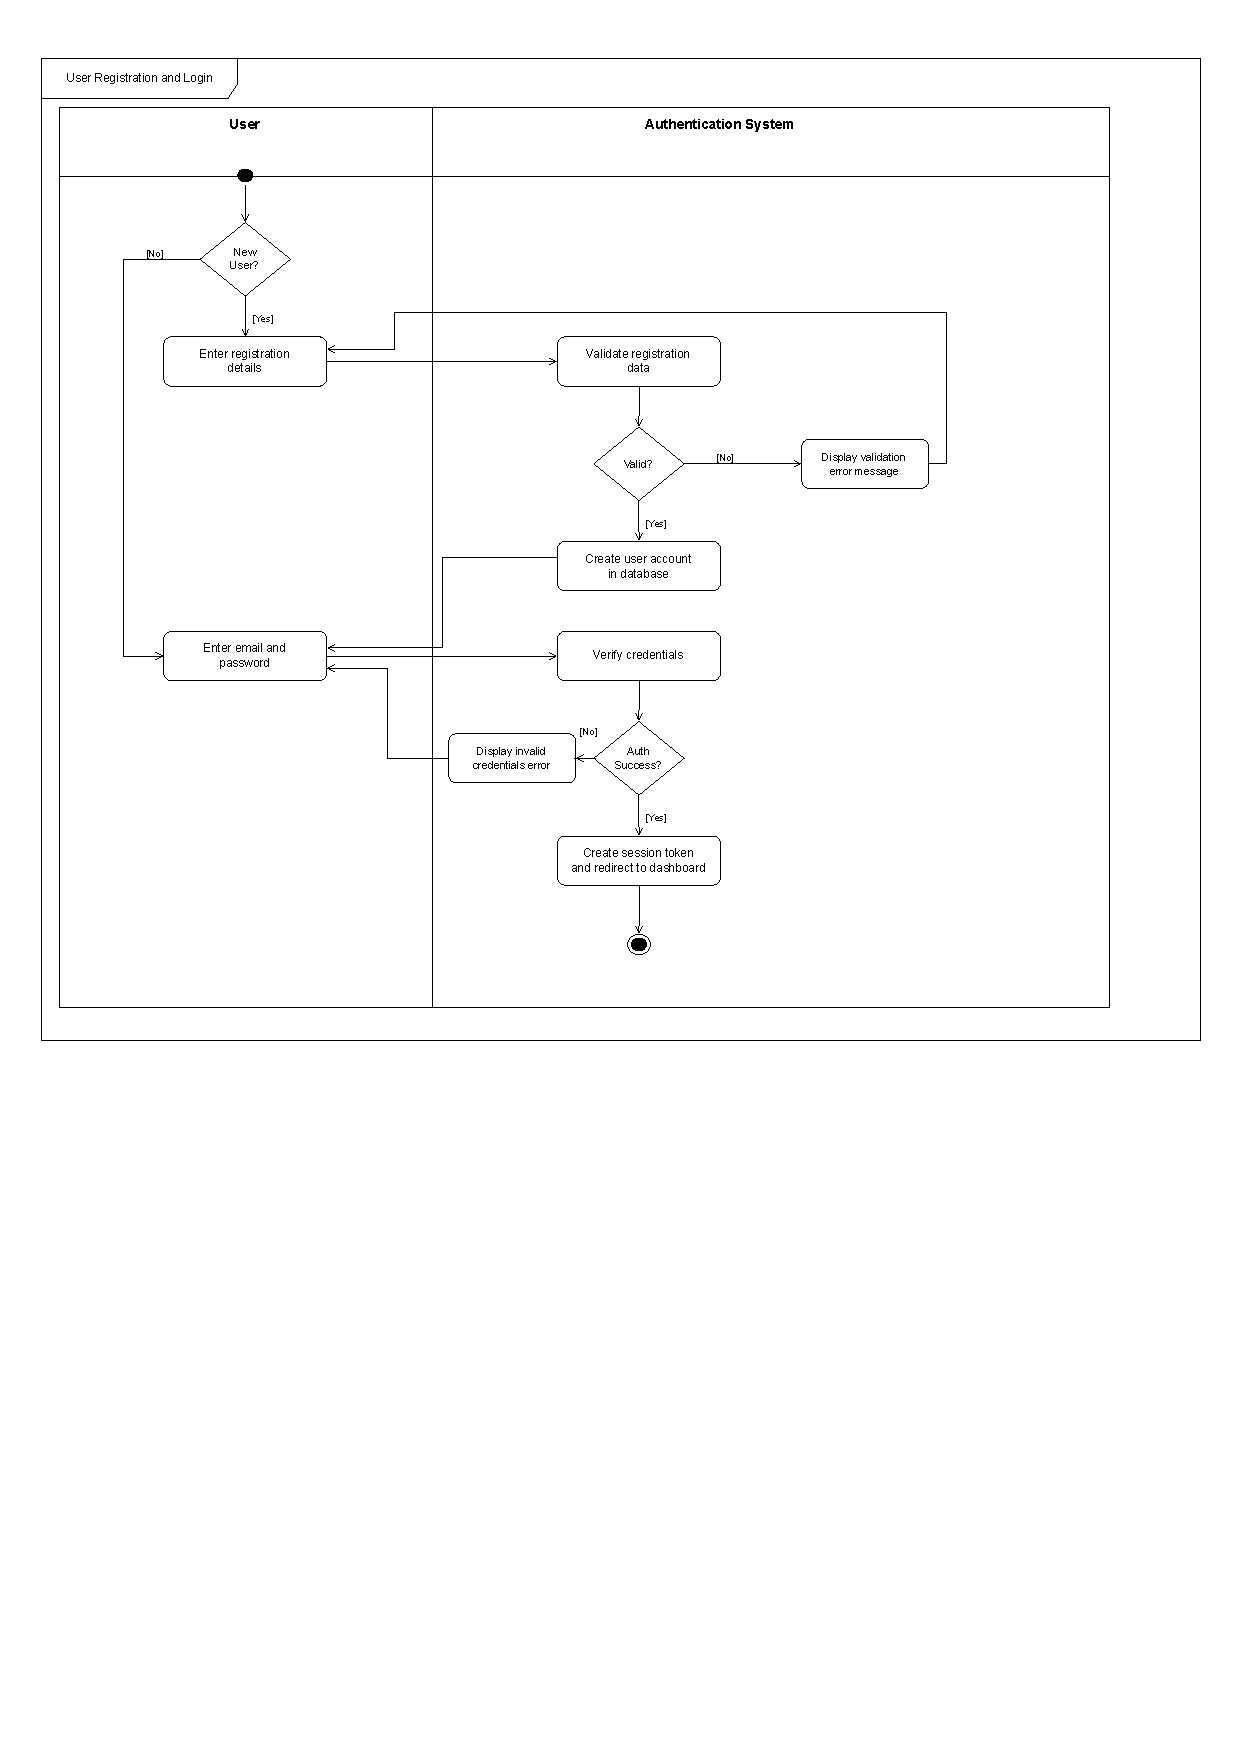
\includegraphics[width=0.55\linewidth]{activity1_fixed.drawio (3).pdf}
    \caption{Activity Diagram: User Registration and Authentication Flow}
    \label{fig:activity1}
\end{figure}

Figure \ref{fig:activity1} depicts the complete user registration and authentication workflow. The process begins when a new user accesses the registration page and submits credentials. The system validates the email format and password strength according to security requirements (minimum 8 characters with mixed case, numbers, and special characters). Upon successful validation, the system creates a hashed password using bcrypt with a cost factor of 12, stores the user account in PostgreSQL, and sends a verification email. For existing users, the authentication flow verifies credentials, generates a JWT token with 24-hour expiration, and establishes a secure session.

\begin{figure}[H]
    \centering
    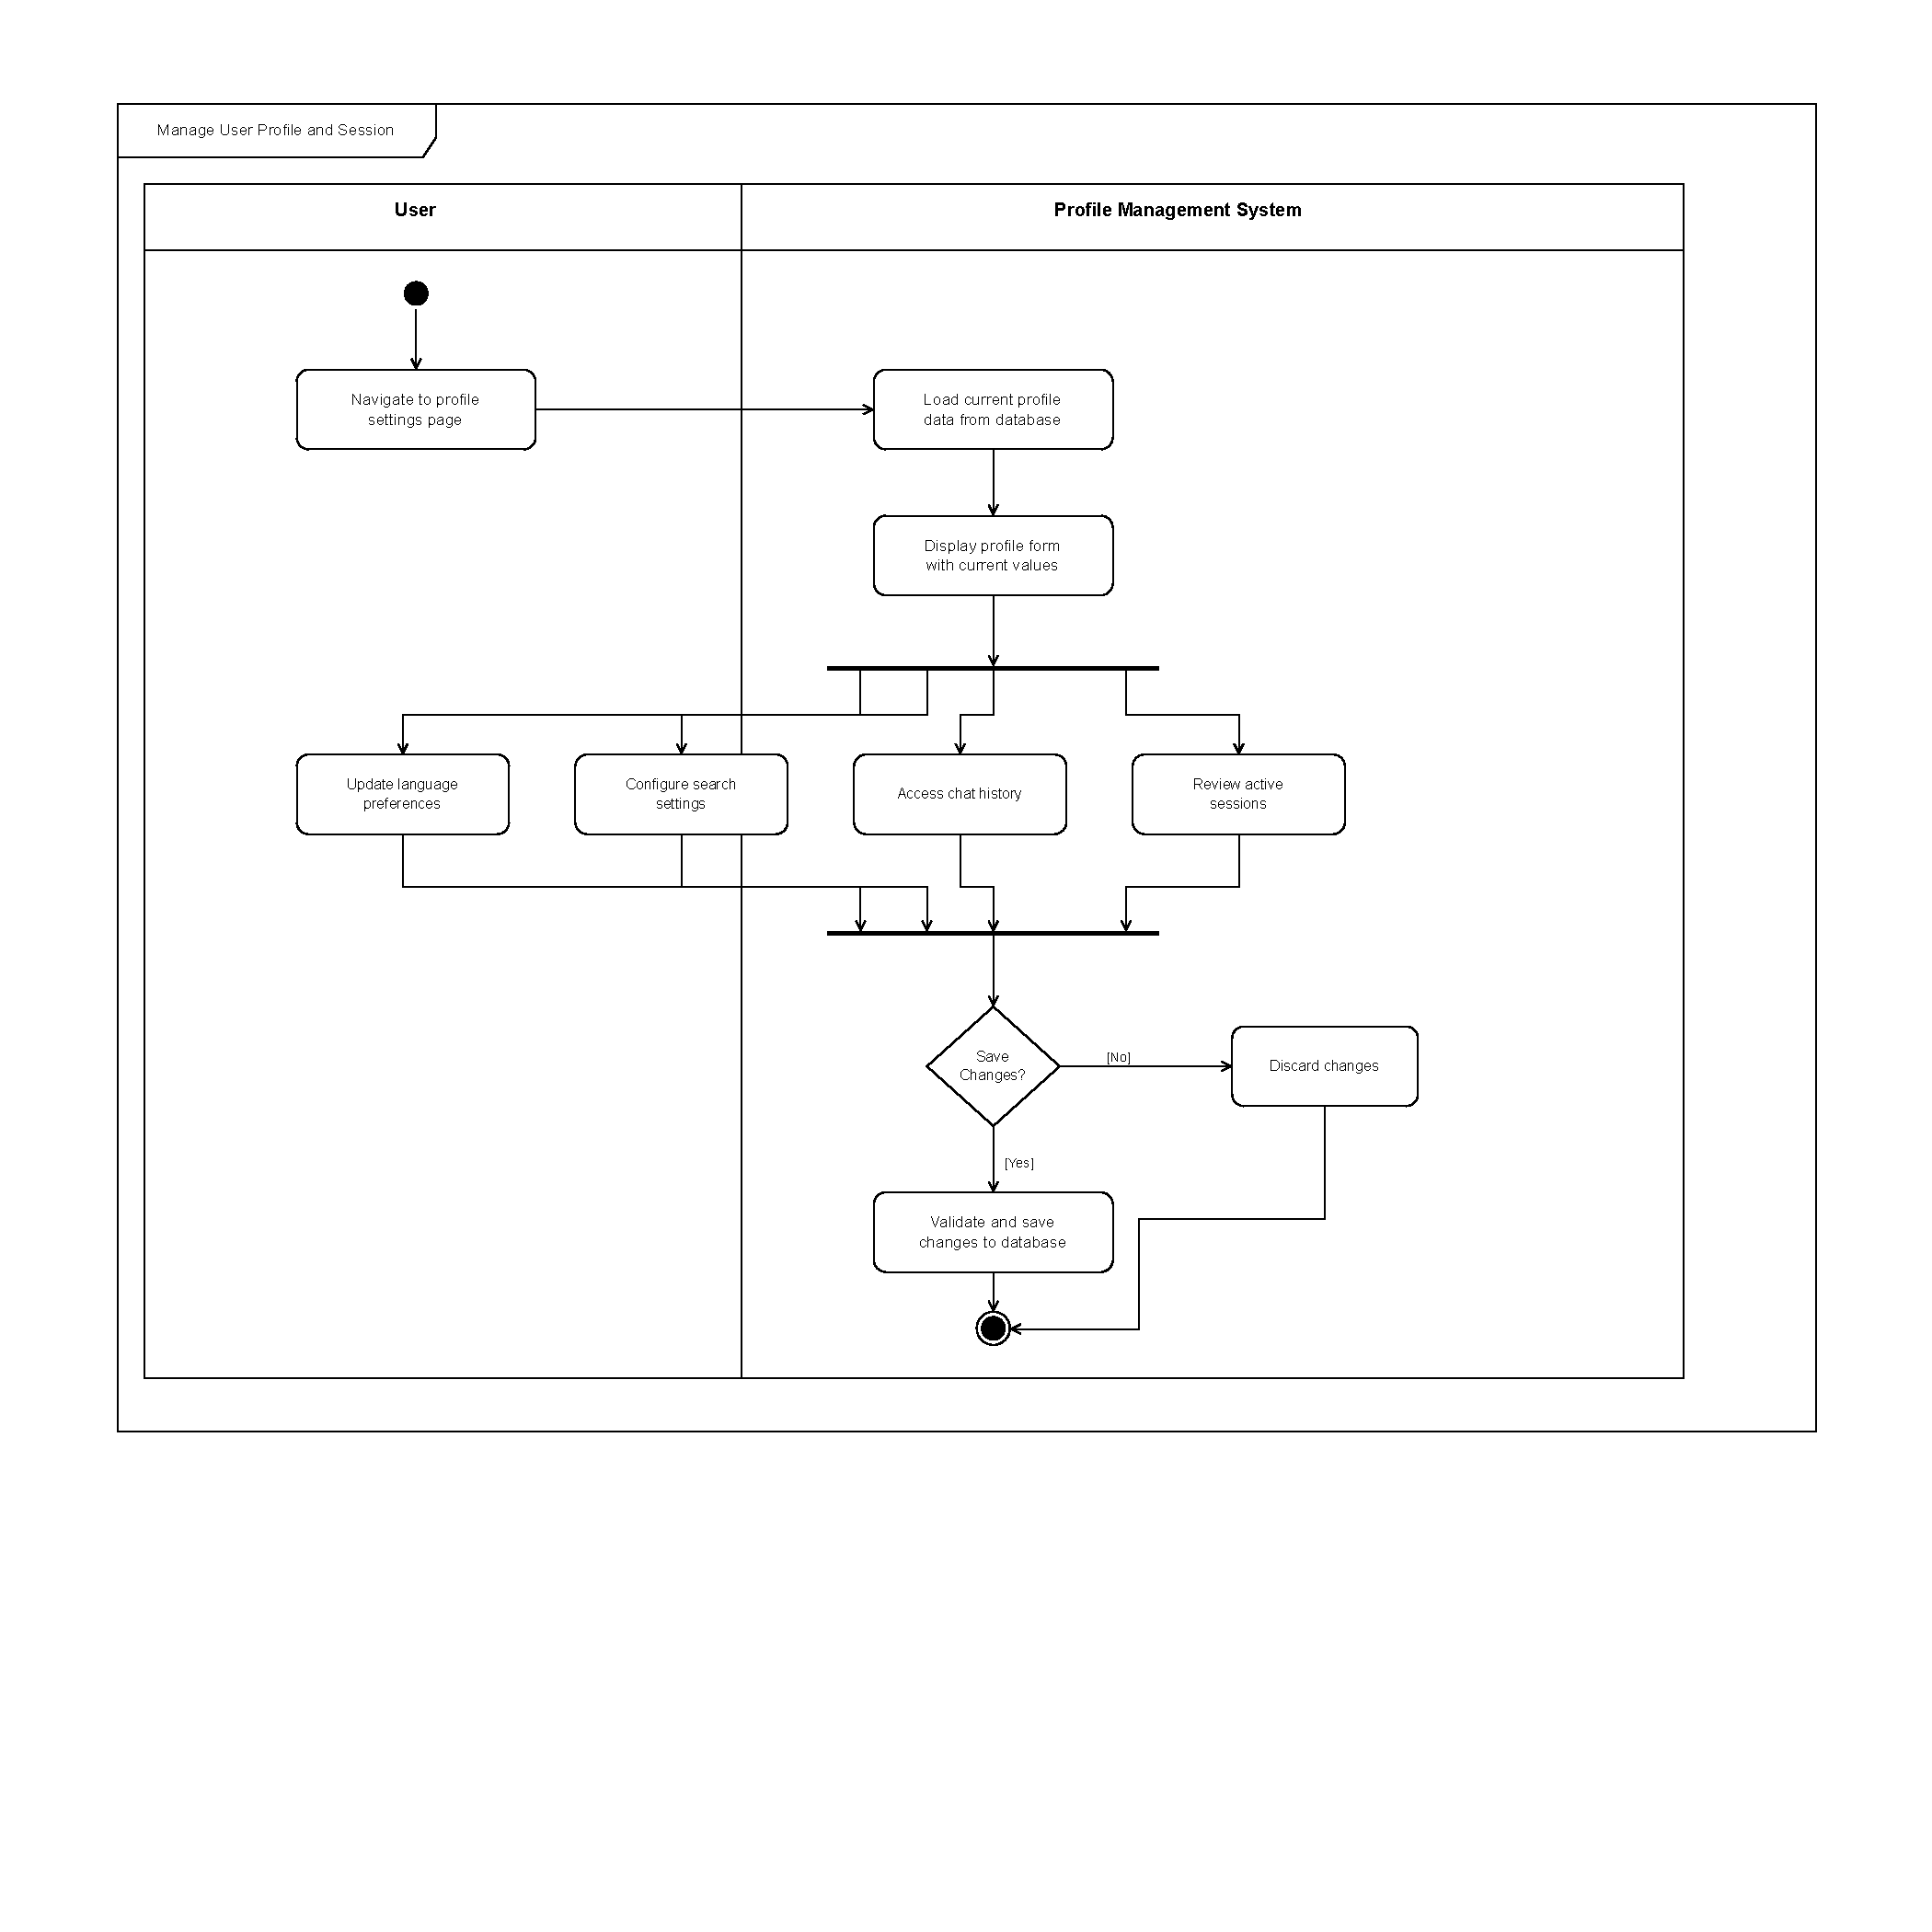
\includegraphics[width=0.55\linewidth]{activity2.drawio.pdf}
    \caption{Activity Diagram: Hybrid Search Execution Flow}
    \label{fig:activity2}
\end{figure}

Figure \ref{fig:activity2} illustrates the hybrid search execution workflow that combines BM25 keyword retrieval with HNSW vector search. When a user submits a query, the system sanitizes the input and triggers parallel execution of two retrieval pathways. The BM25 path tokenizes the query, retrieves posting lists from the inverted index, and scores documents using probabilistic relevance formulas. Simultaneously, the vector path encodes the query using Sentence-BERT, performs approximate nearest neighbor search on the HNSW graph, and returns top candidates based on cosine similarity. The Reciprocal Rank Fusion algorithm then merges both result sets, producing a unified ranking that leverages lexical precision and semantic understanding.

\begin{figure}[H]
    \centering
    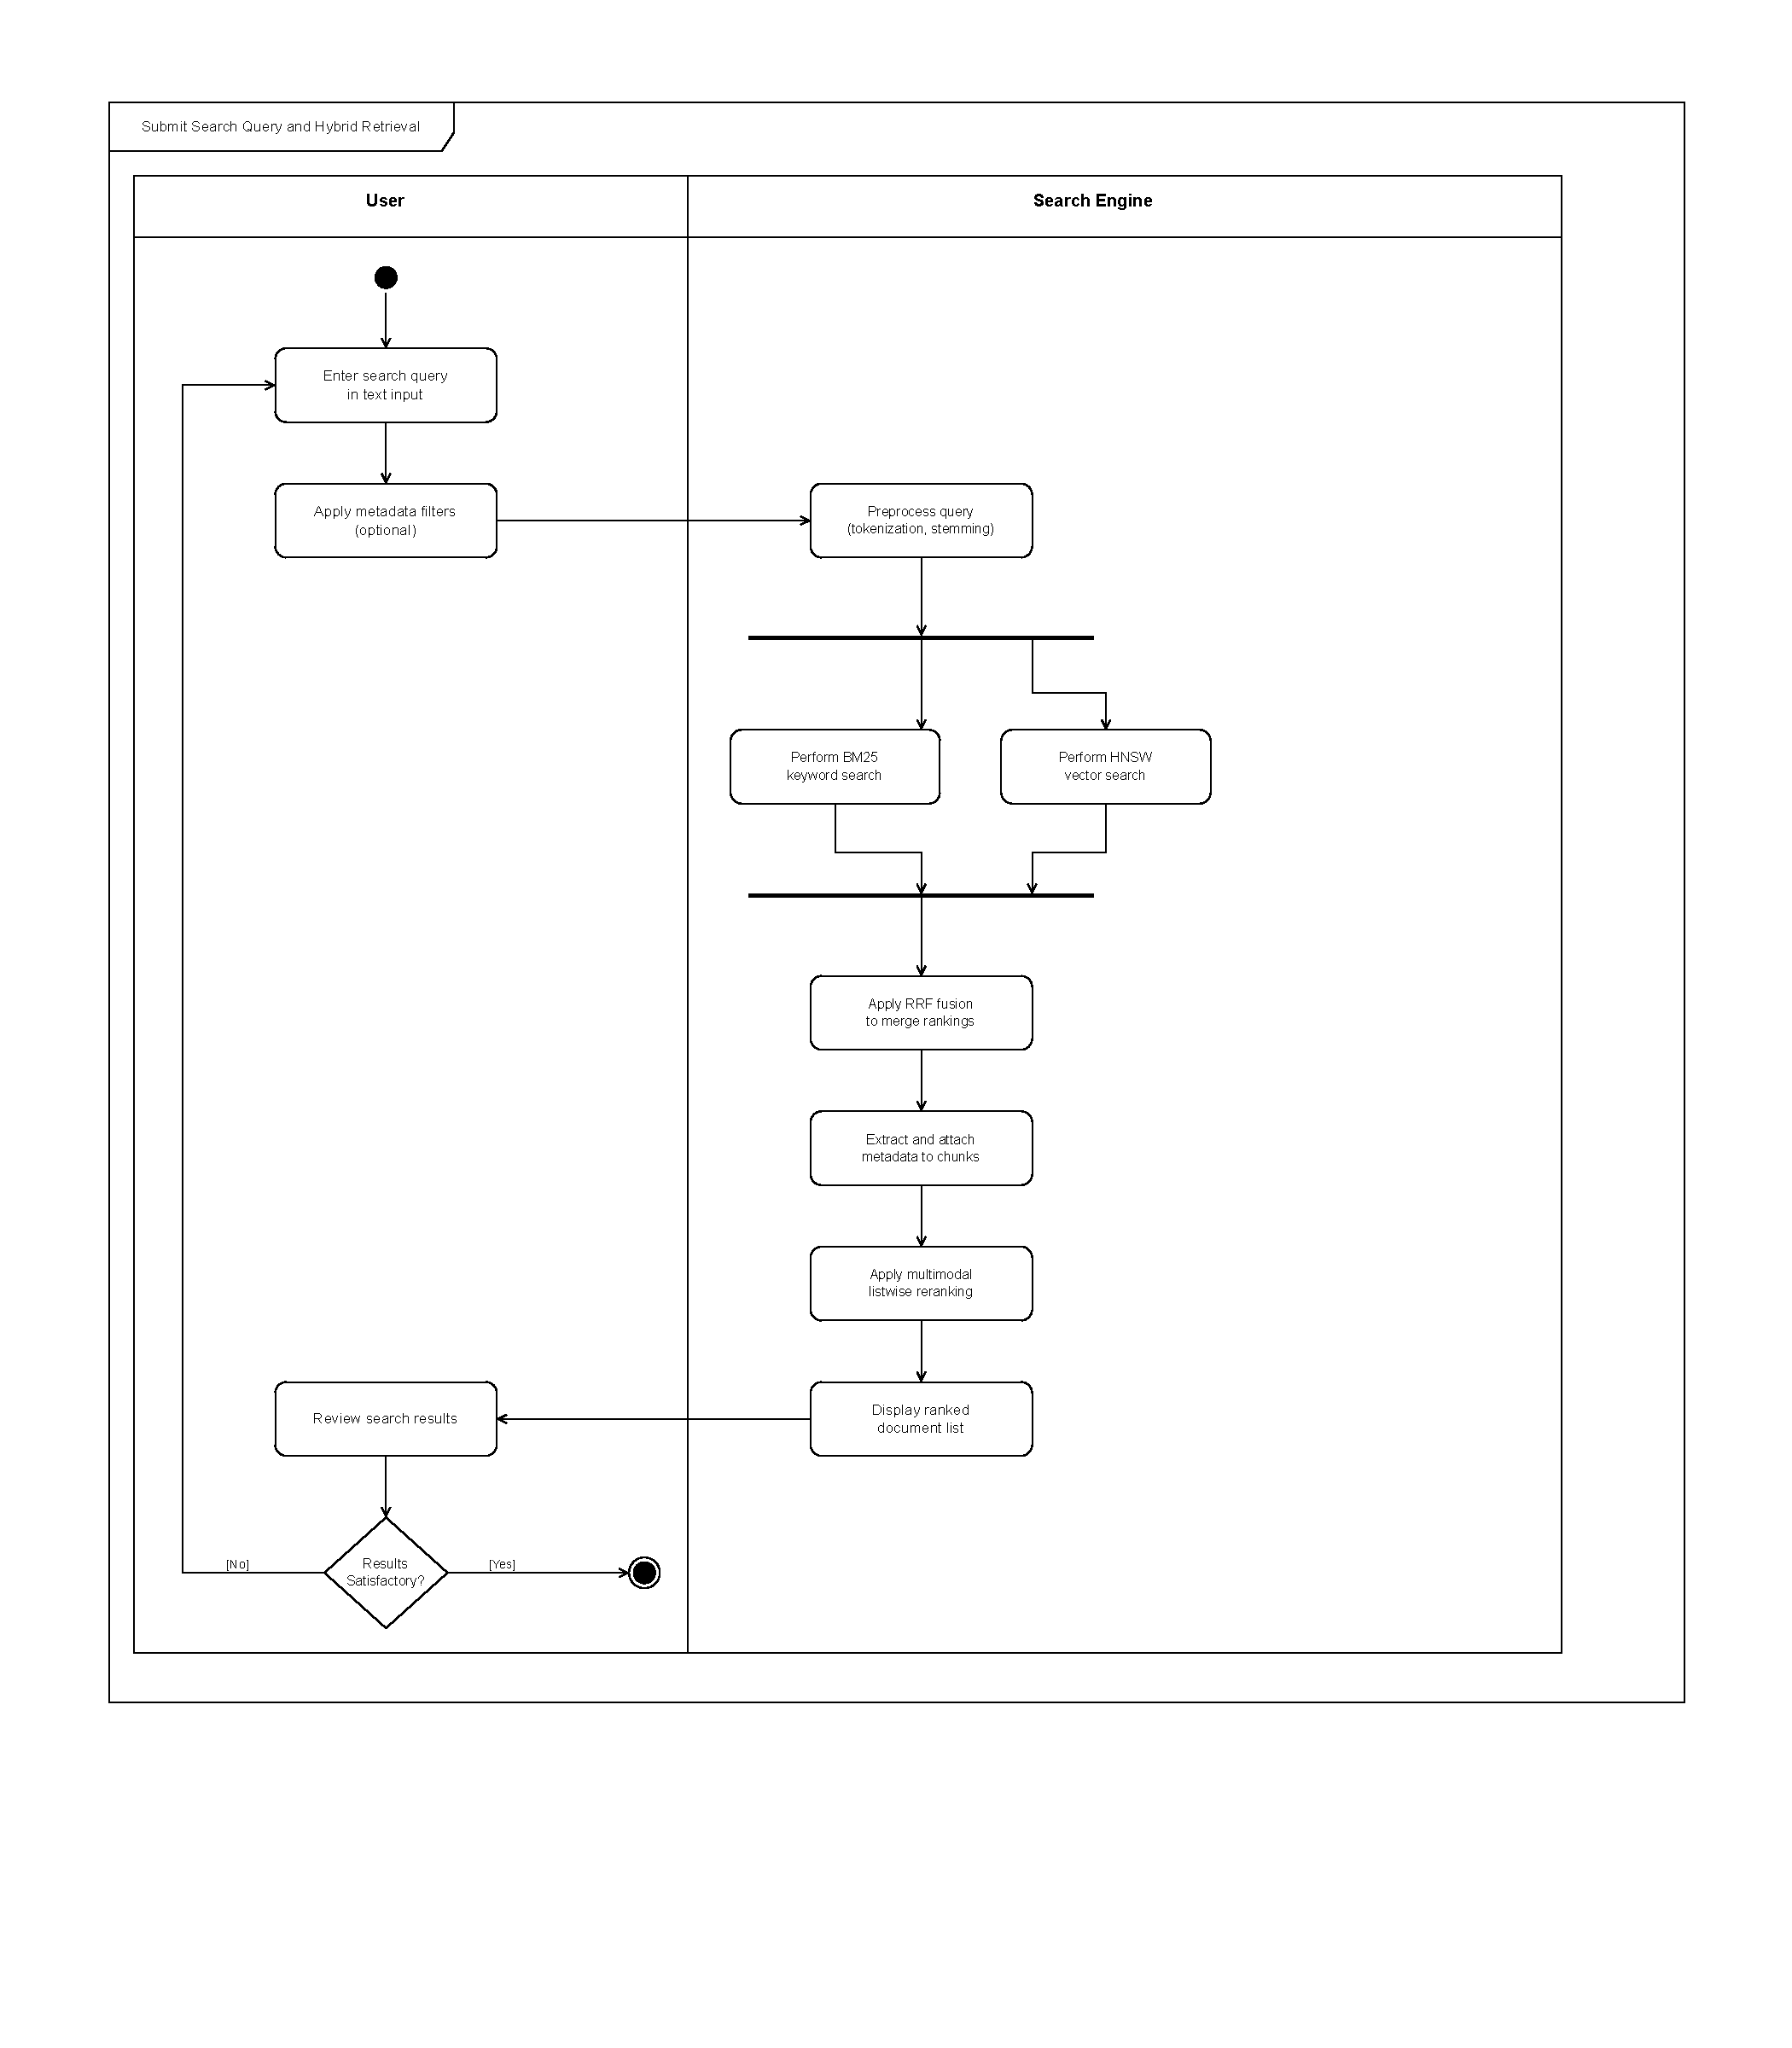
\includegraphics[width=0.55\linewidth]{activity3.drawio.pdf}
    \caption{Activity Diagram: Multimodal Reranking Process}
    \label{fig:activity3}
\end{figure}

Figure \ref{fig:activity3} details the multimodal reranking process using BLIP-2. After hybrid search produces top 20 candidates, the system retrieves associated images for each document. The reranker constructs a setwise prompt containing the query, document texts, and image references. BLIP-2's Q-Former architecture processes cross-modal interactions, encoding both textual semantics and visual content. The vision-language model evaluates each candidate's multimodal relevance, generating a reranked list that considers whether charts, diagrams, or other visual elements address the user's information need. This enables the system to properly rank technical documentation where critical information resides in visual components.

\begin{figure}[H]
    \centering
    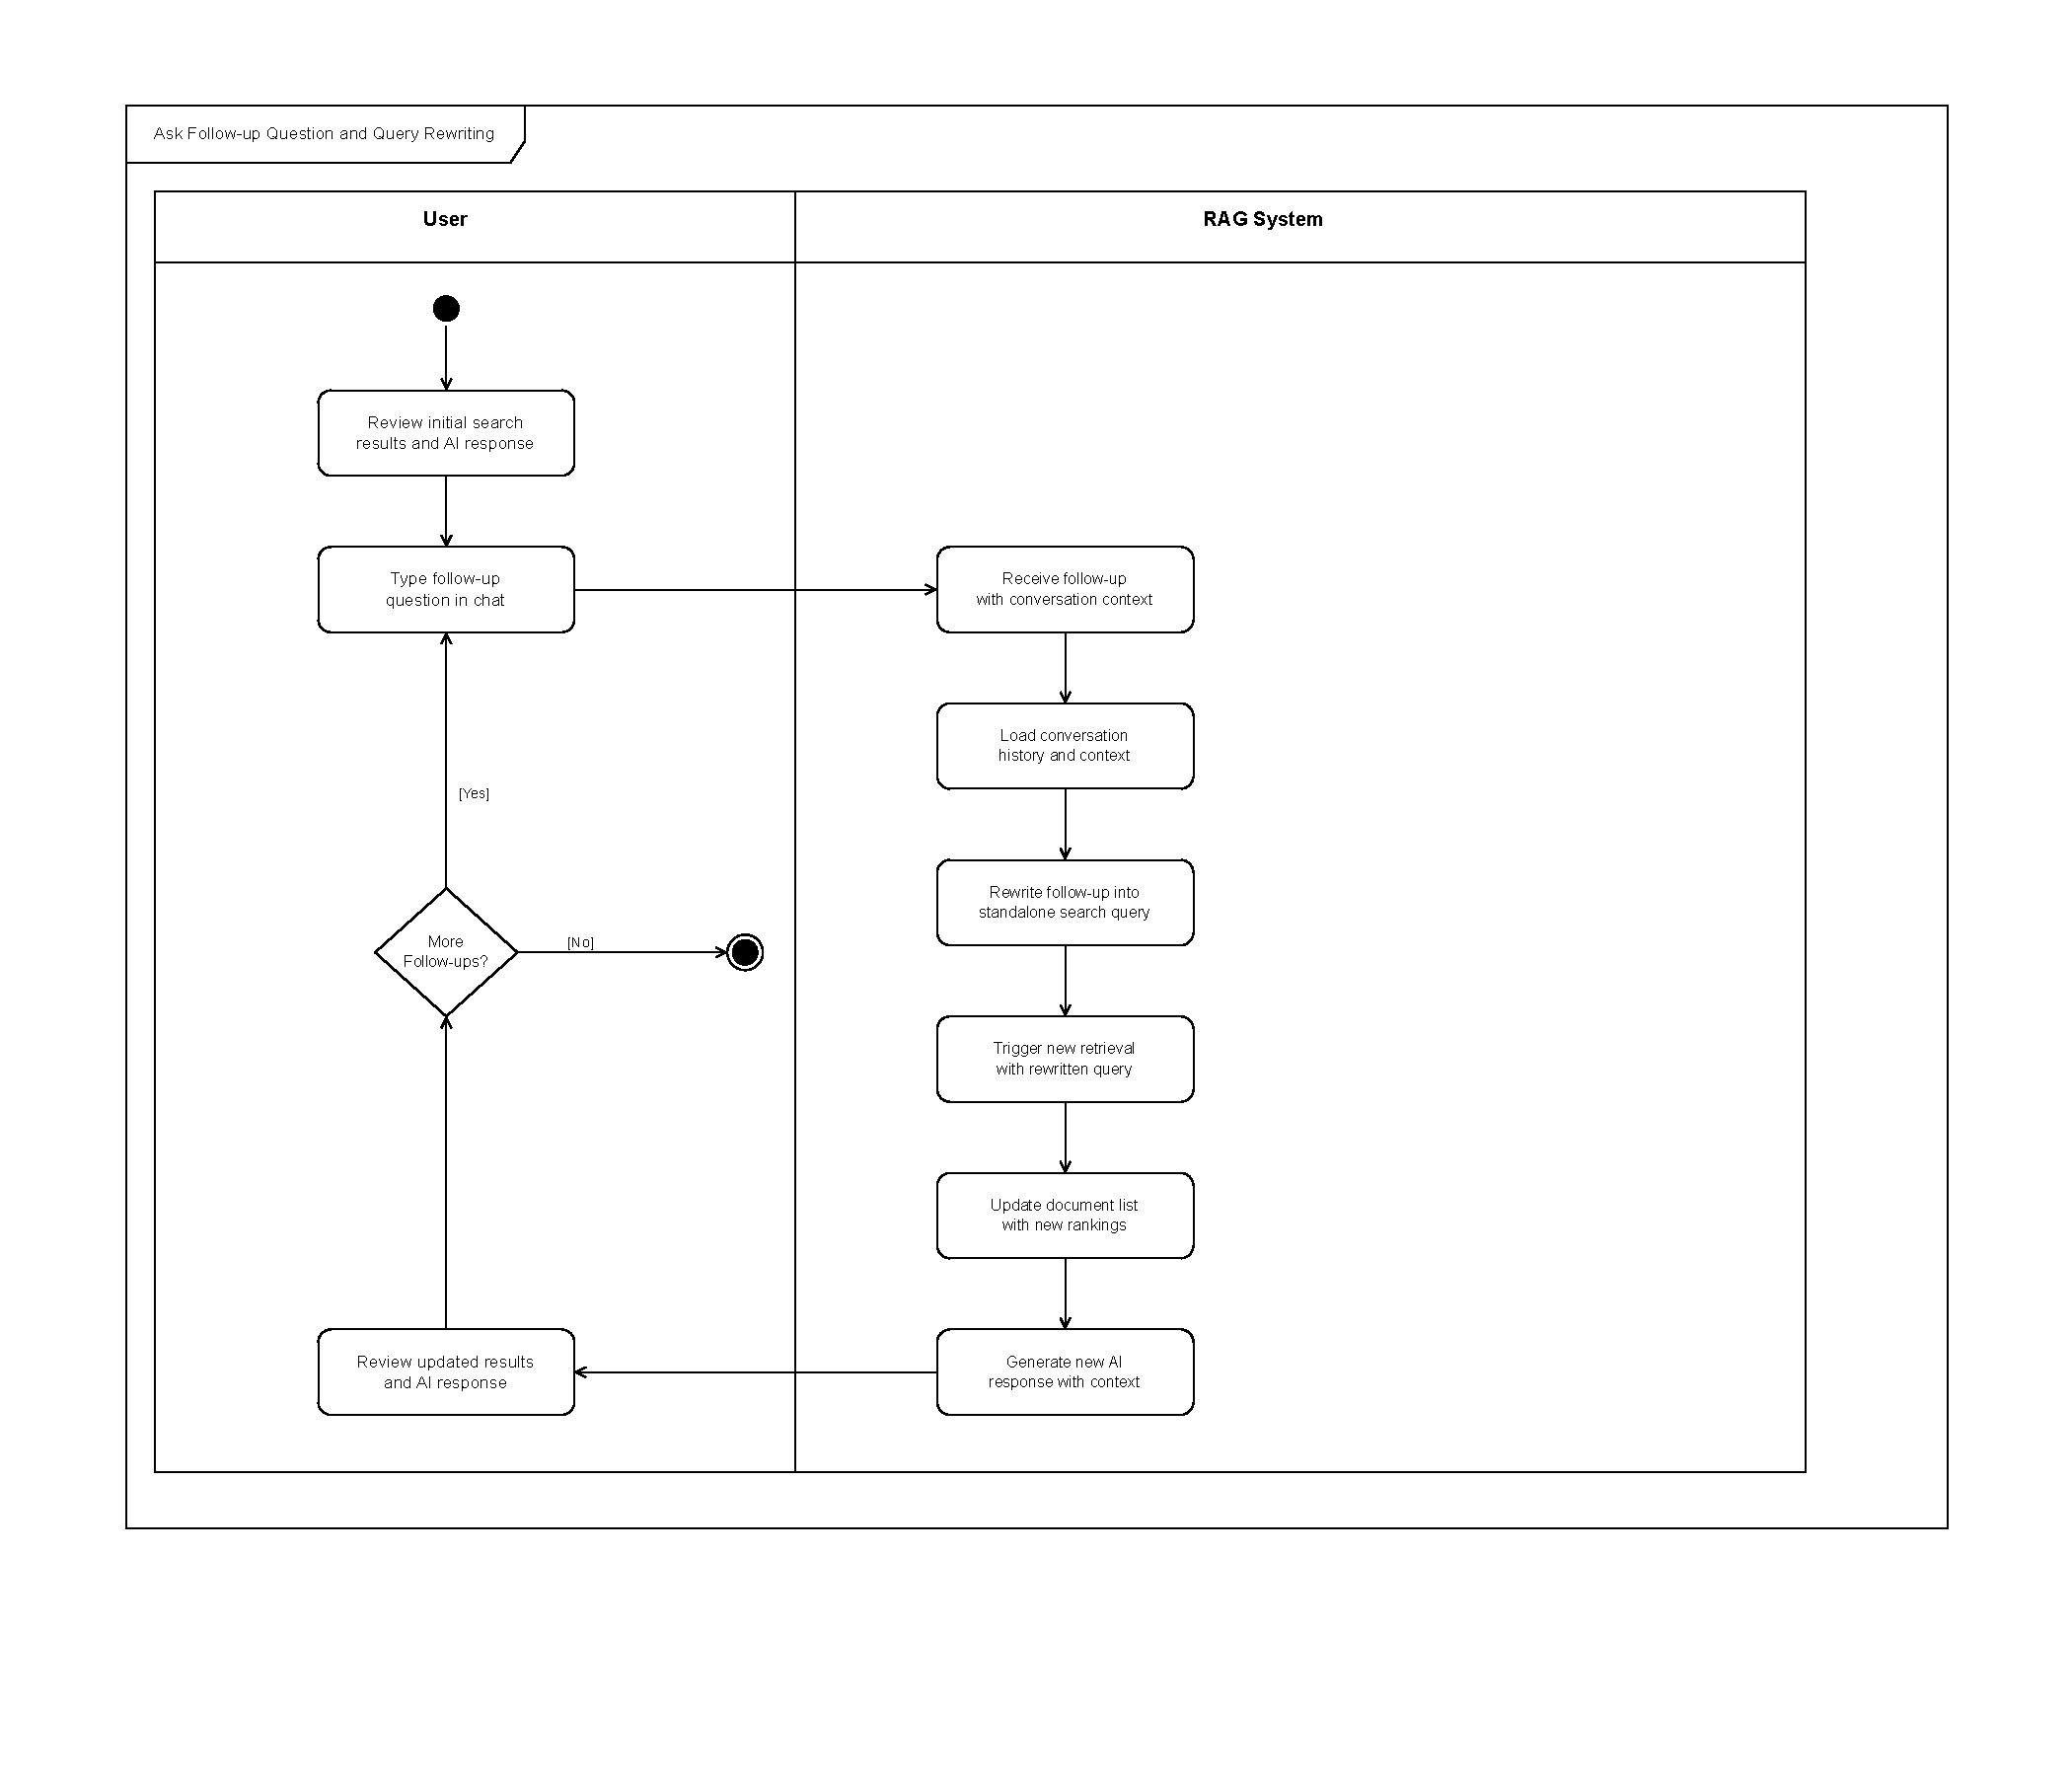
\includegraphics[width=0.55\linewidth]{activity4.drawio.pdf}
    \caption{Activity Diagram: Distributed Crawling Workflow}
    \label{fig:activity4}
\end{figure}

Figure \ref{fig:activity4} shows the distributed crawling coordination mechanism using Kafka. When an administrator triggers a crawl job, the coordinator partitions tasks across configured data sources (Confluence spaces, Google Drive folders, Git repositories, network shares). Tasks are published to the "crawl-tasks" Kafka topic, and worker nodes consume assignments based on availability. Each worker authenticates with its assigned source, recursively fetches documents while respecting rate limits, extracts text and images, and publishes results to the "documents-ingested" topic. Failed tasks trigger exponential backoff retries before being marked as failed. This architecture enables horizontal scaling by simply adding worker nodes to handle larger document collections.

\begin{figure}[H]
    \centering
    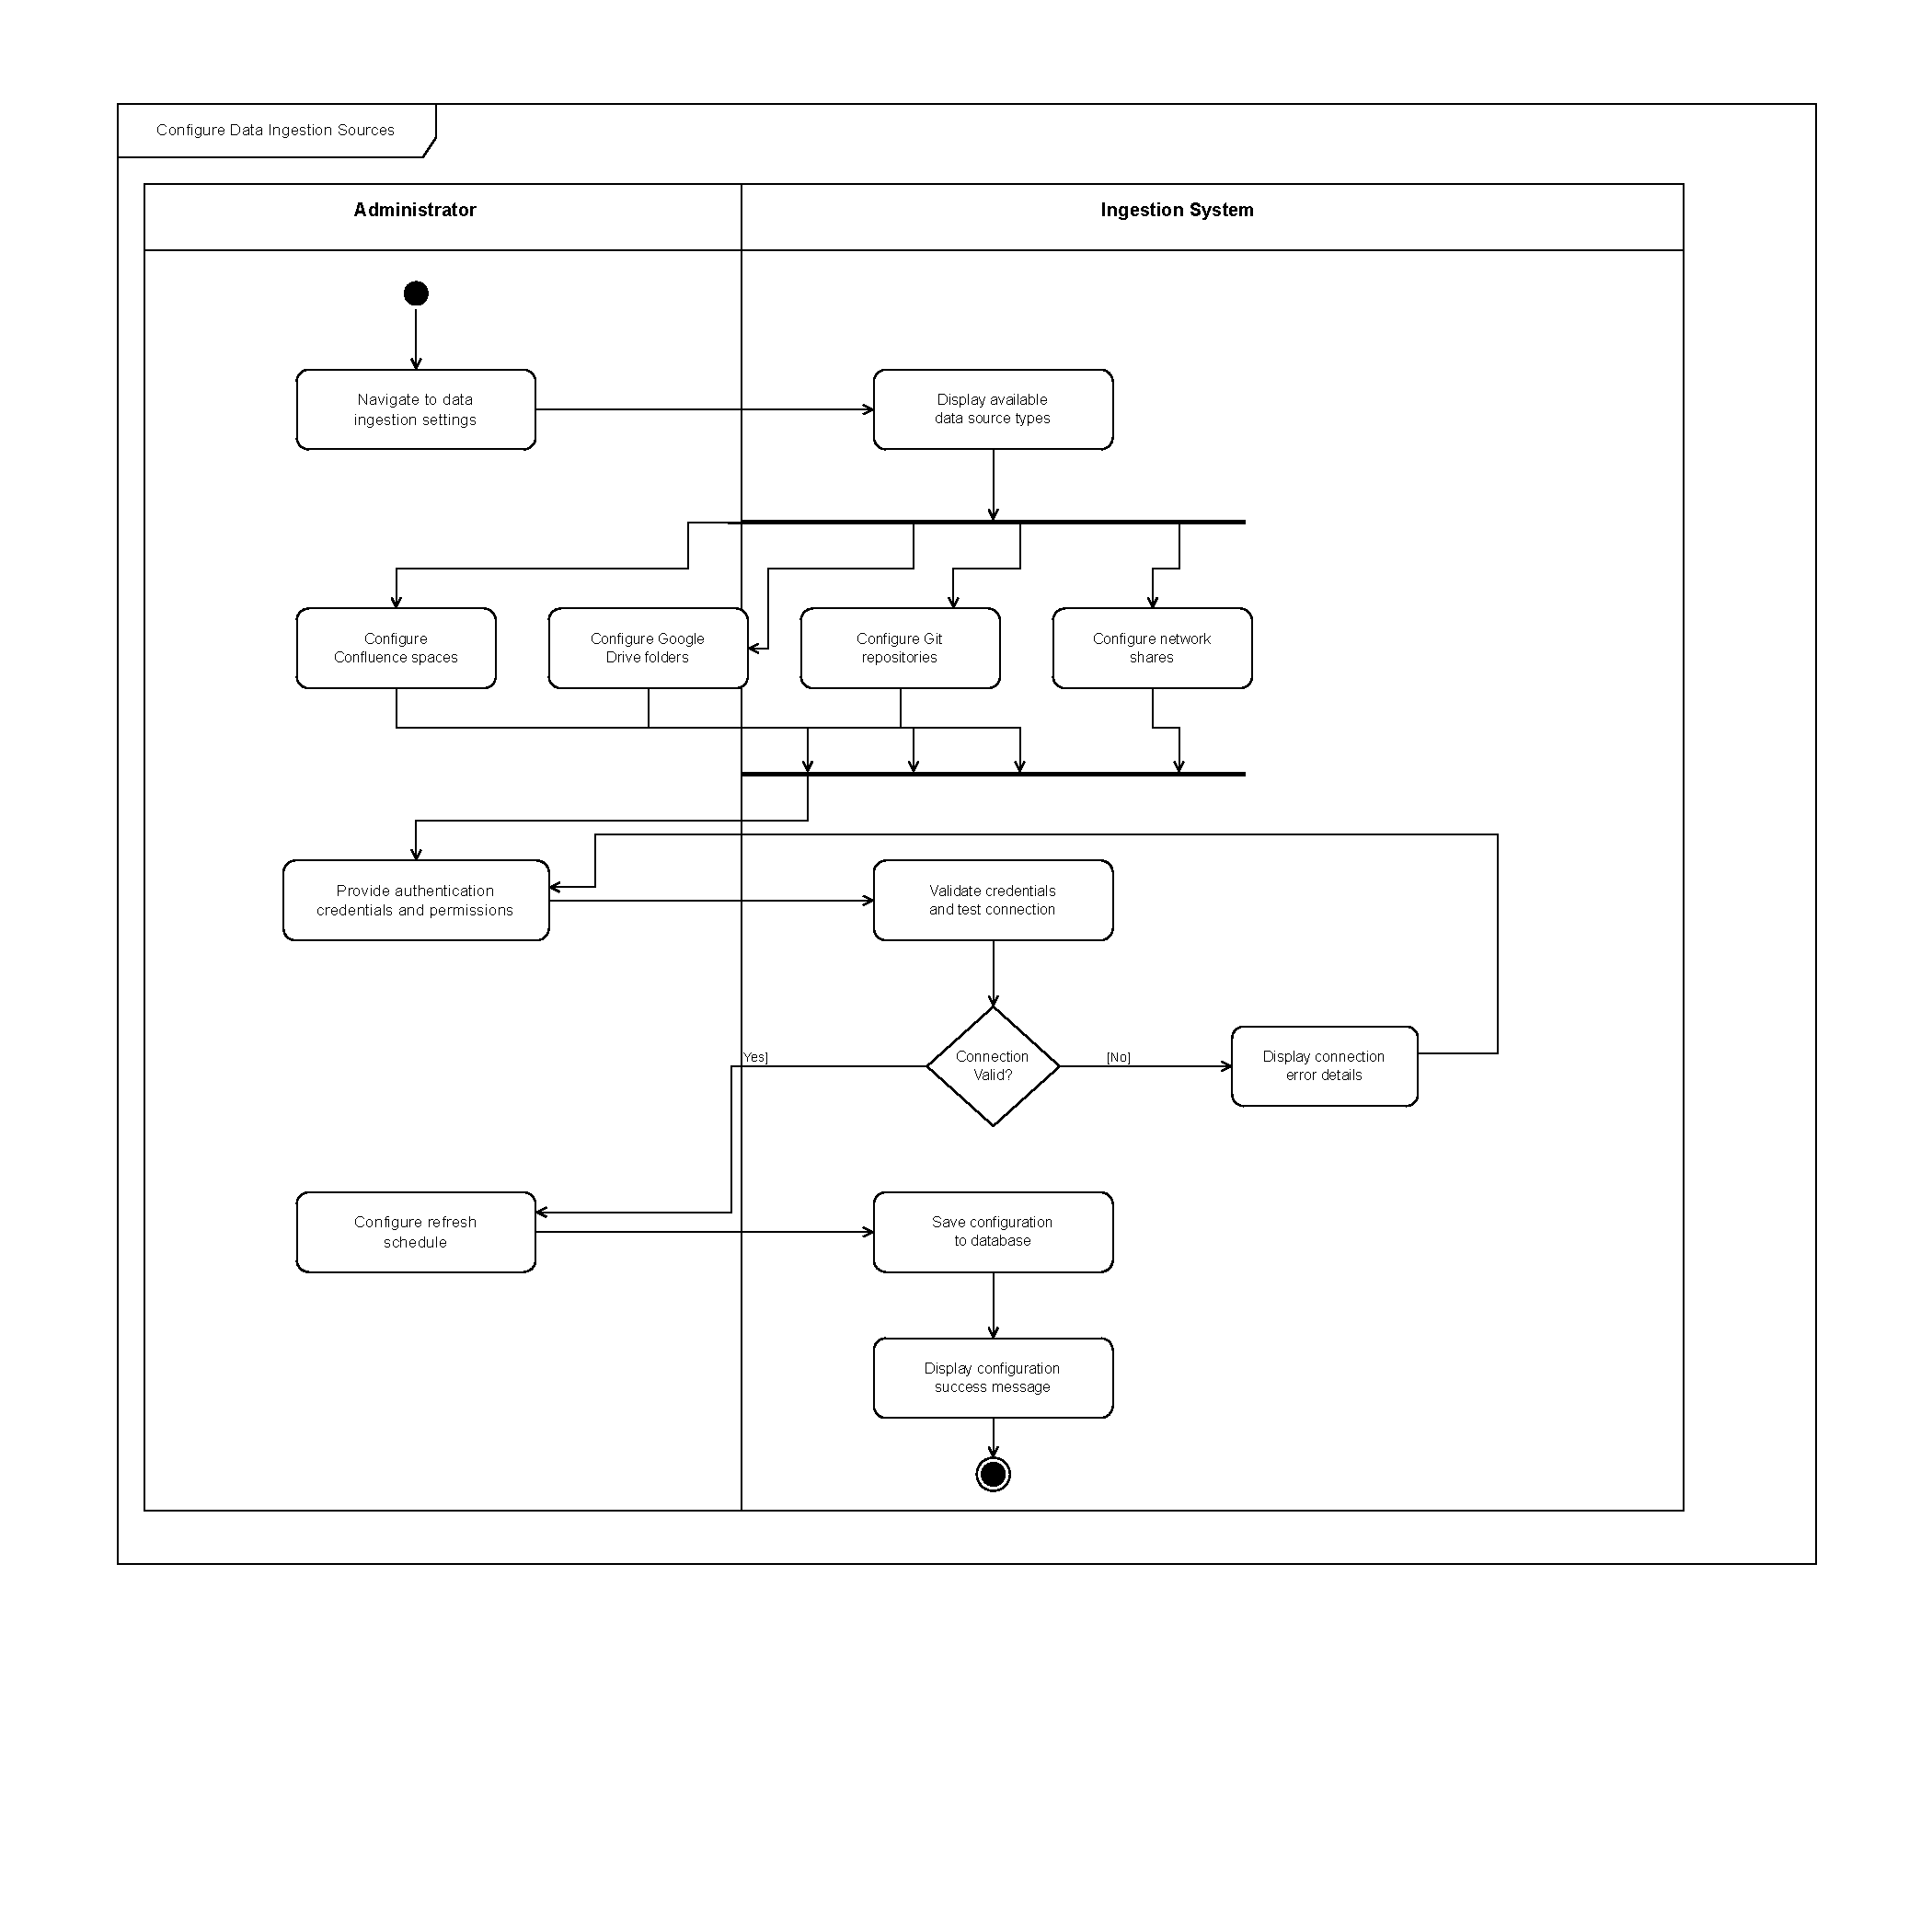
\includegraphics[width=0.55\linewidth]{activity5.drawio.pdf}
    \caption{Activity Diagram: Document Chunking and Embedding Generation}
    \label{fig:activity5}
\end{figure}

Figure \ref{fig:activity5} illustrates the document processing pipeline from ingestion to index building. Documents consumed from Kafka undergo format-specific extraction (PDF, DOCX, HTML) to separate text and images. The chunking module segments text into semantic units using heading structure, paragraph boundaries, or fixed token counts, maintaining 10\% overlap between adjacent chunks to preserve context. Text chunks are batched and encoded using Sentence-BERT on GPU, while images are processed through CLIP's vision encoder. Generated embeddings are inserted into the HNSW vector index, and document metadata is stored in PostgreSQL. This pipeline processes thousands of documents per hour using GPU acceleration and batch optimization.

\begin{figure}[H]
    \centering
    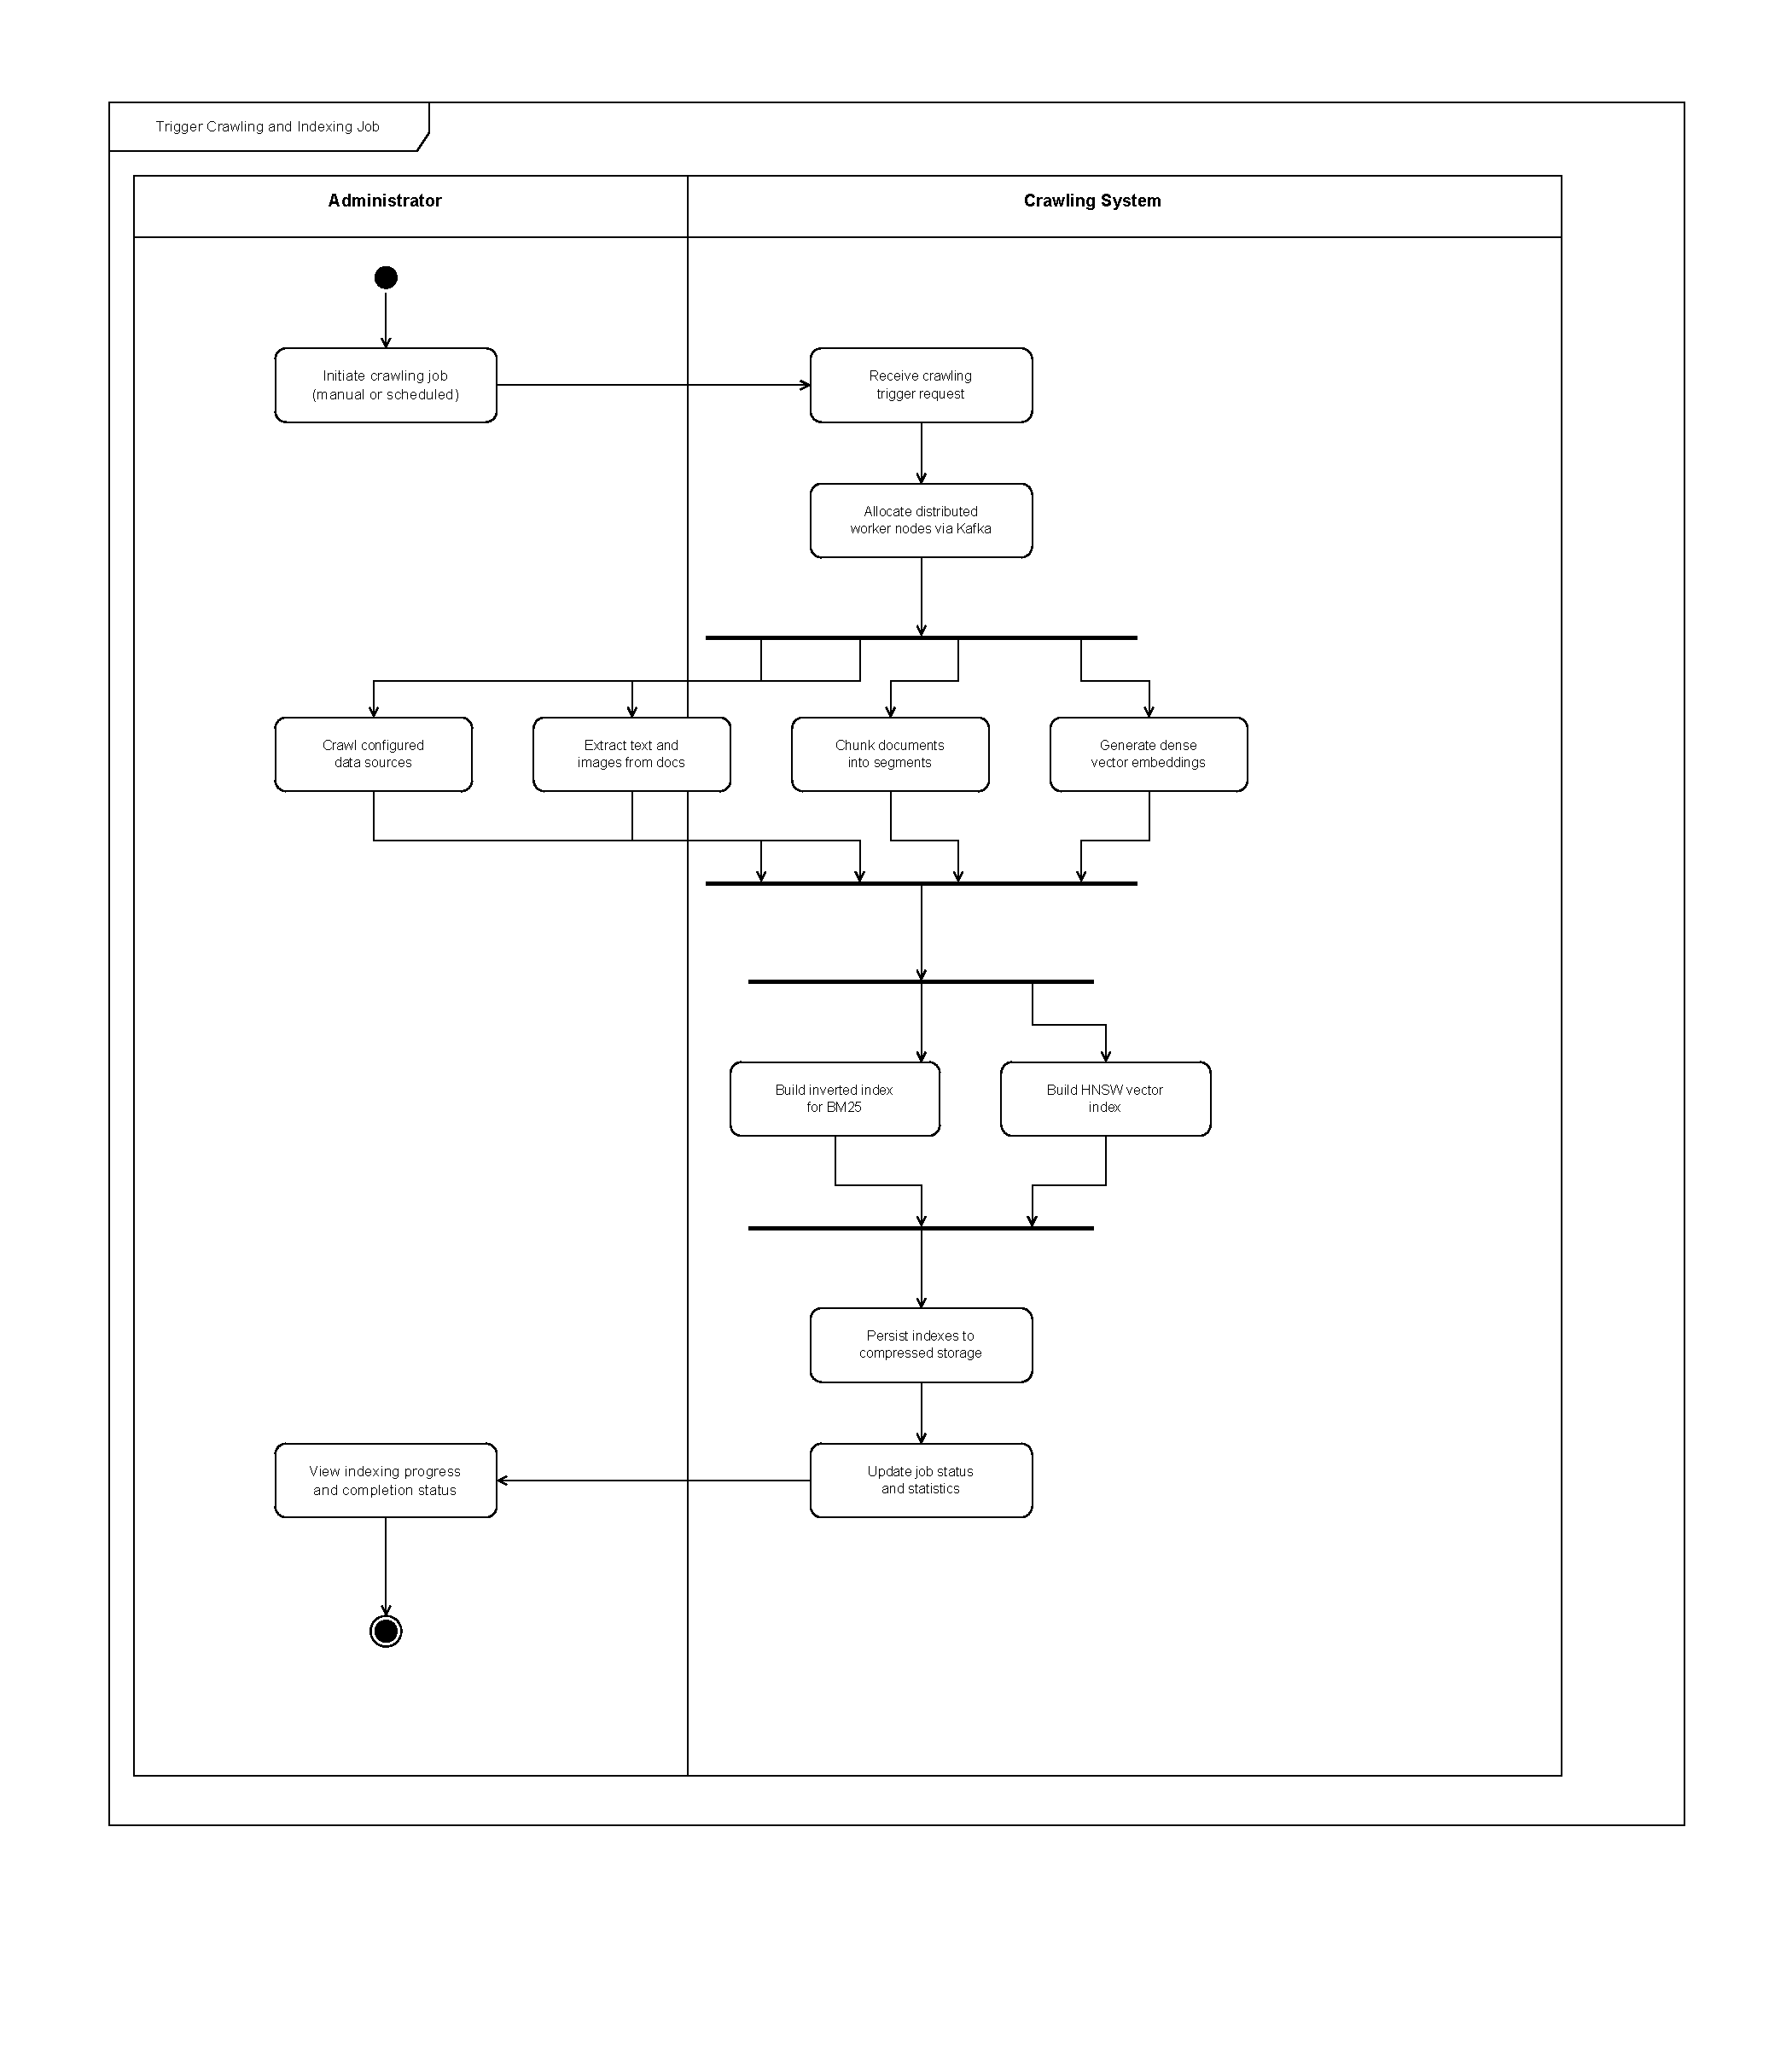
\includegraphics[width=0.55\linewidth]{activity6.drawio.pdf}
    \caption{Activity Diagram: RAG Answer Generation with Citations}
    \label{fig:activity6}
\end{figure}

Figure \ref{fig:activity6} depicts the retrieval-augmented generation workflow for producing grounded answers. Upon receiving a user query, the system executes the retrieval pipeline to fetch top K=5 most relevant chunks. These chunks are formatted into a structured prompt with clear delimiters and source identifiers. The system prompt explicitly instructs the LLM to answer based solely on provided context and to cite sources using [1], [2] notation. The LLM generates a response via SGLang, which streams tokens to the user interface in real-time. The system performs post-generation validation using an entailment model to verify claims against sources, flagging any unsupported assertions for review.

\begin{figure}[H]
    \centering
    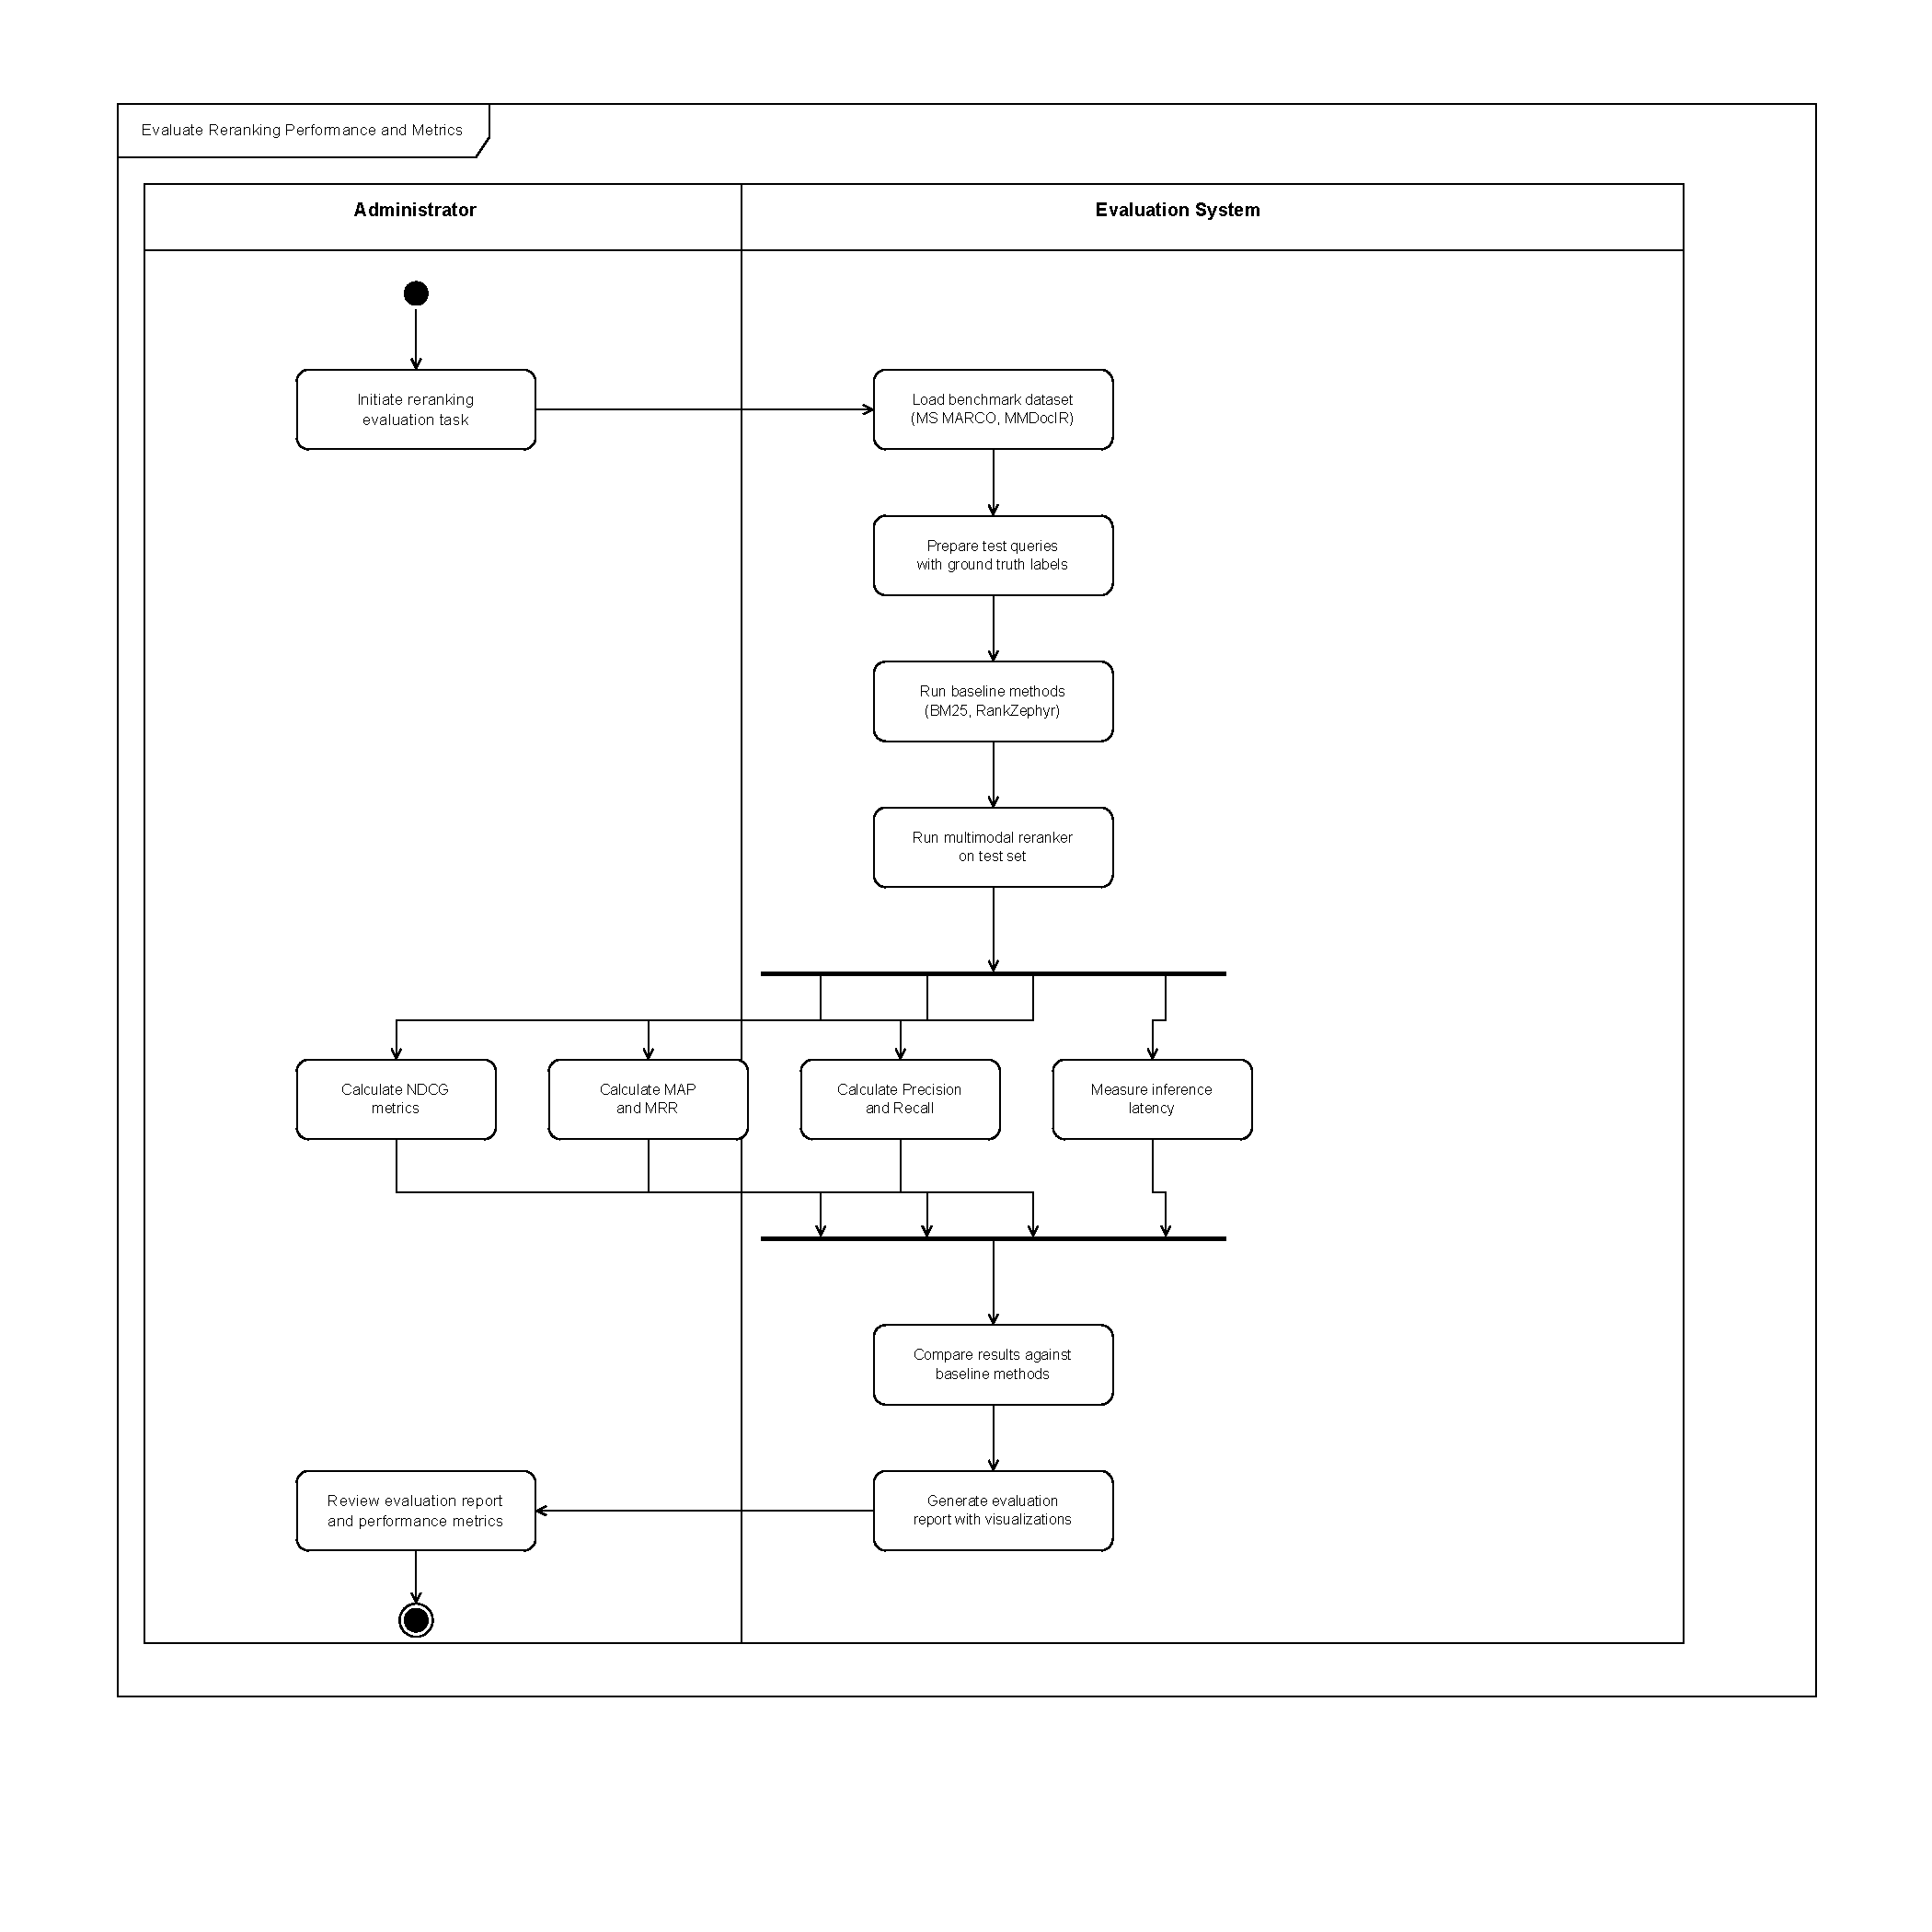
\includegraphics[width=0.55\linewidth]{activity7.drawio.pdf}
    \caption{Activity Diagram: Conversational Query Rewriting Flow}
    \label{fig:activity7}
\end{figure}

Figure \ref{fig:activity7} shows the conversational query rewriting mechanism that enables iterative search refinement. When the system detects a follow-up question (e.g., "What about performance optimization?"), it retrieves the last 10 conversation turns from Redis. These turns, along with the new query, are formatted into a rewriting prompt asking the LLM to produce a standalone query that captures the user's intent without requiring conversation context. The LLM generates the rewritten query, which triggers a new retrieval cycle. This closed-loop architecture allows the search system to continually improve results based on user interactions, creating an iterative exploration experience where each question builds upon previous findings.

\begin{figure}[H]
    \centering
    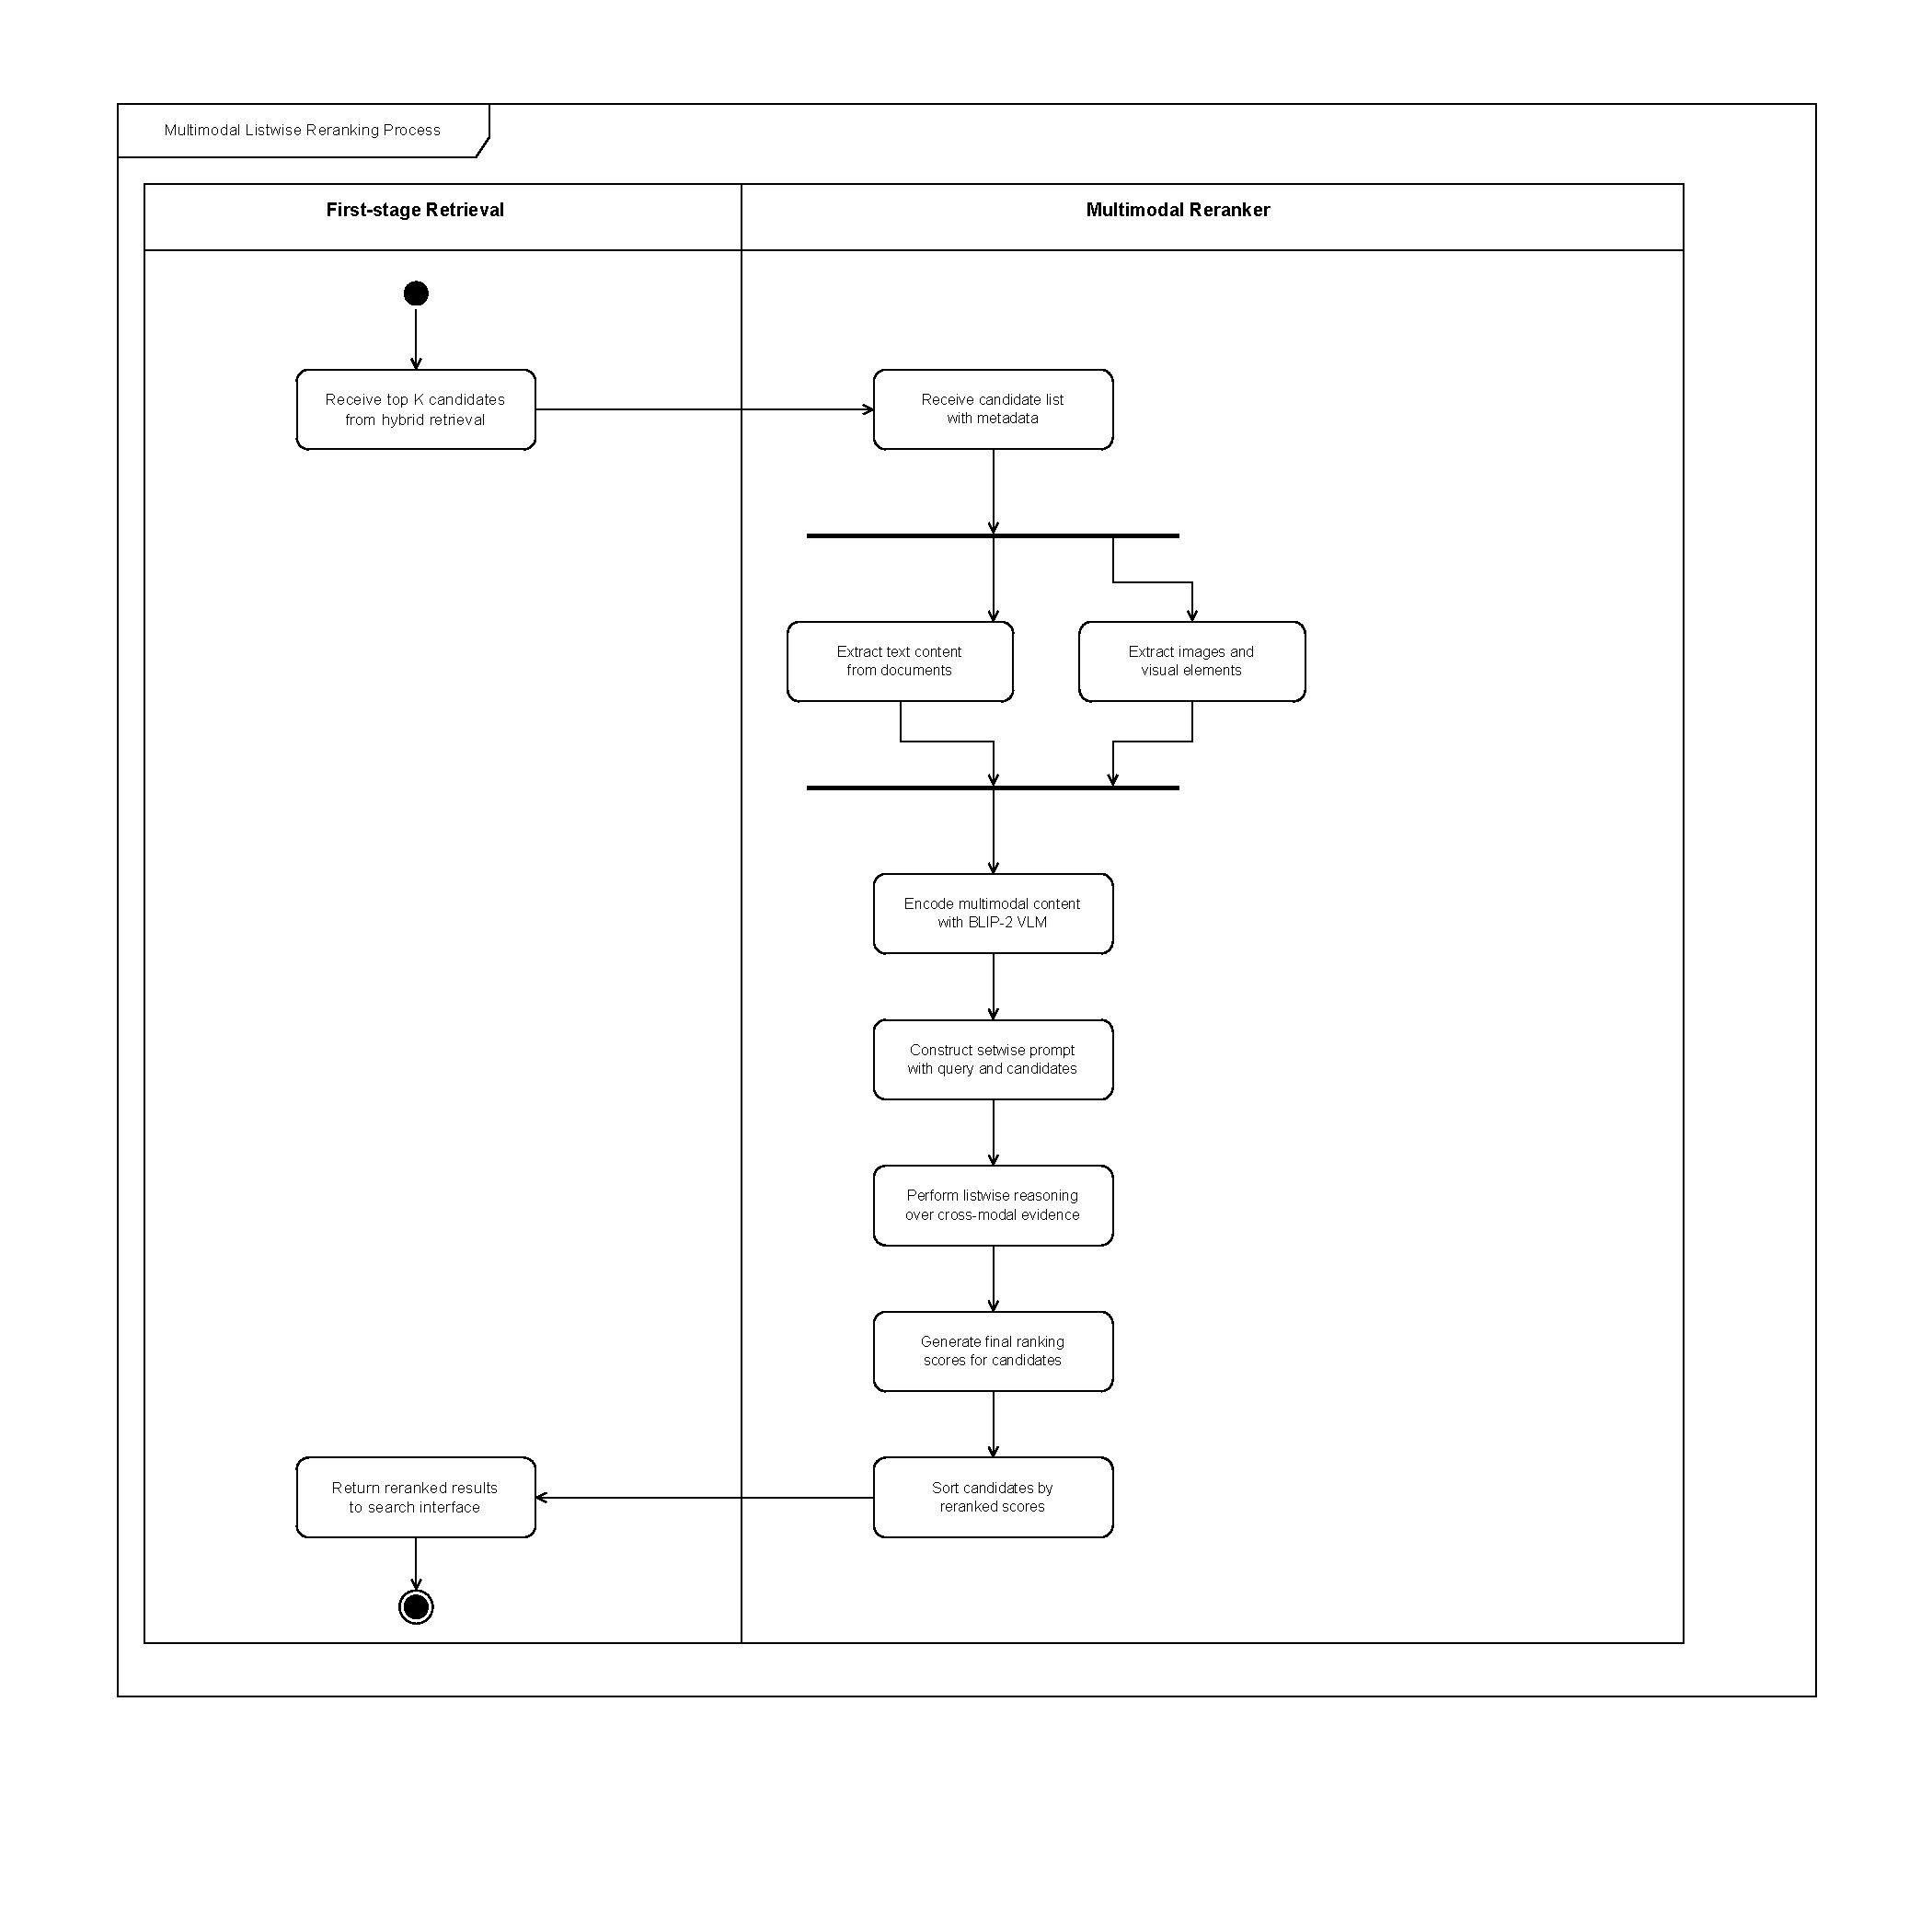
\includegraphics[width=0.55\linewidth]{activity8.drawio.pdf}
    \caption{Activity Diagram: Index Building and Refresh Process}
    \label{fig:activity8}
\end{figure}

Figure \ref{fig:activity8} illustrates the index building and refresh workflow. During initial indexing, the system processes all documents from configured sources, generating embeddings and building both inverted (BM25) and vector (HNSW) indices. For incremental updates, the system retrieves only documents modified since the last crawl timestamp, computes embeddings for new content, and merges them into existing indices using FAISS's add\_with\_ids method. The inverted index is updated by appending new term posting lists. After index updates complete, the system performs atomic swaps to replace the serving indices without downtime, ensuring continuous query availability. Index versions are tracked in PostgreSQL, enabling rollback if update issues arise.

\begin{figure}[H]
    \centering
    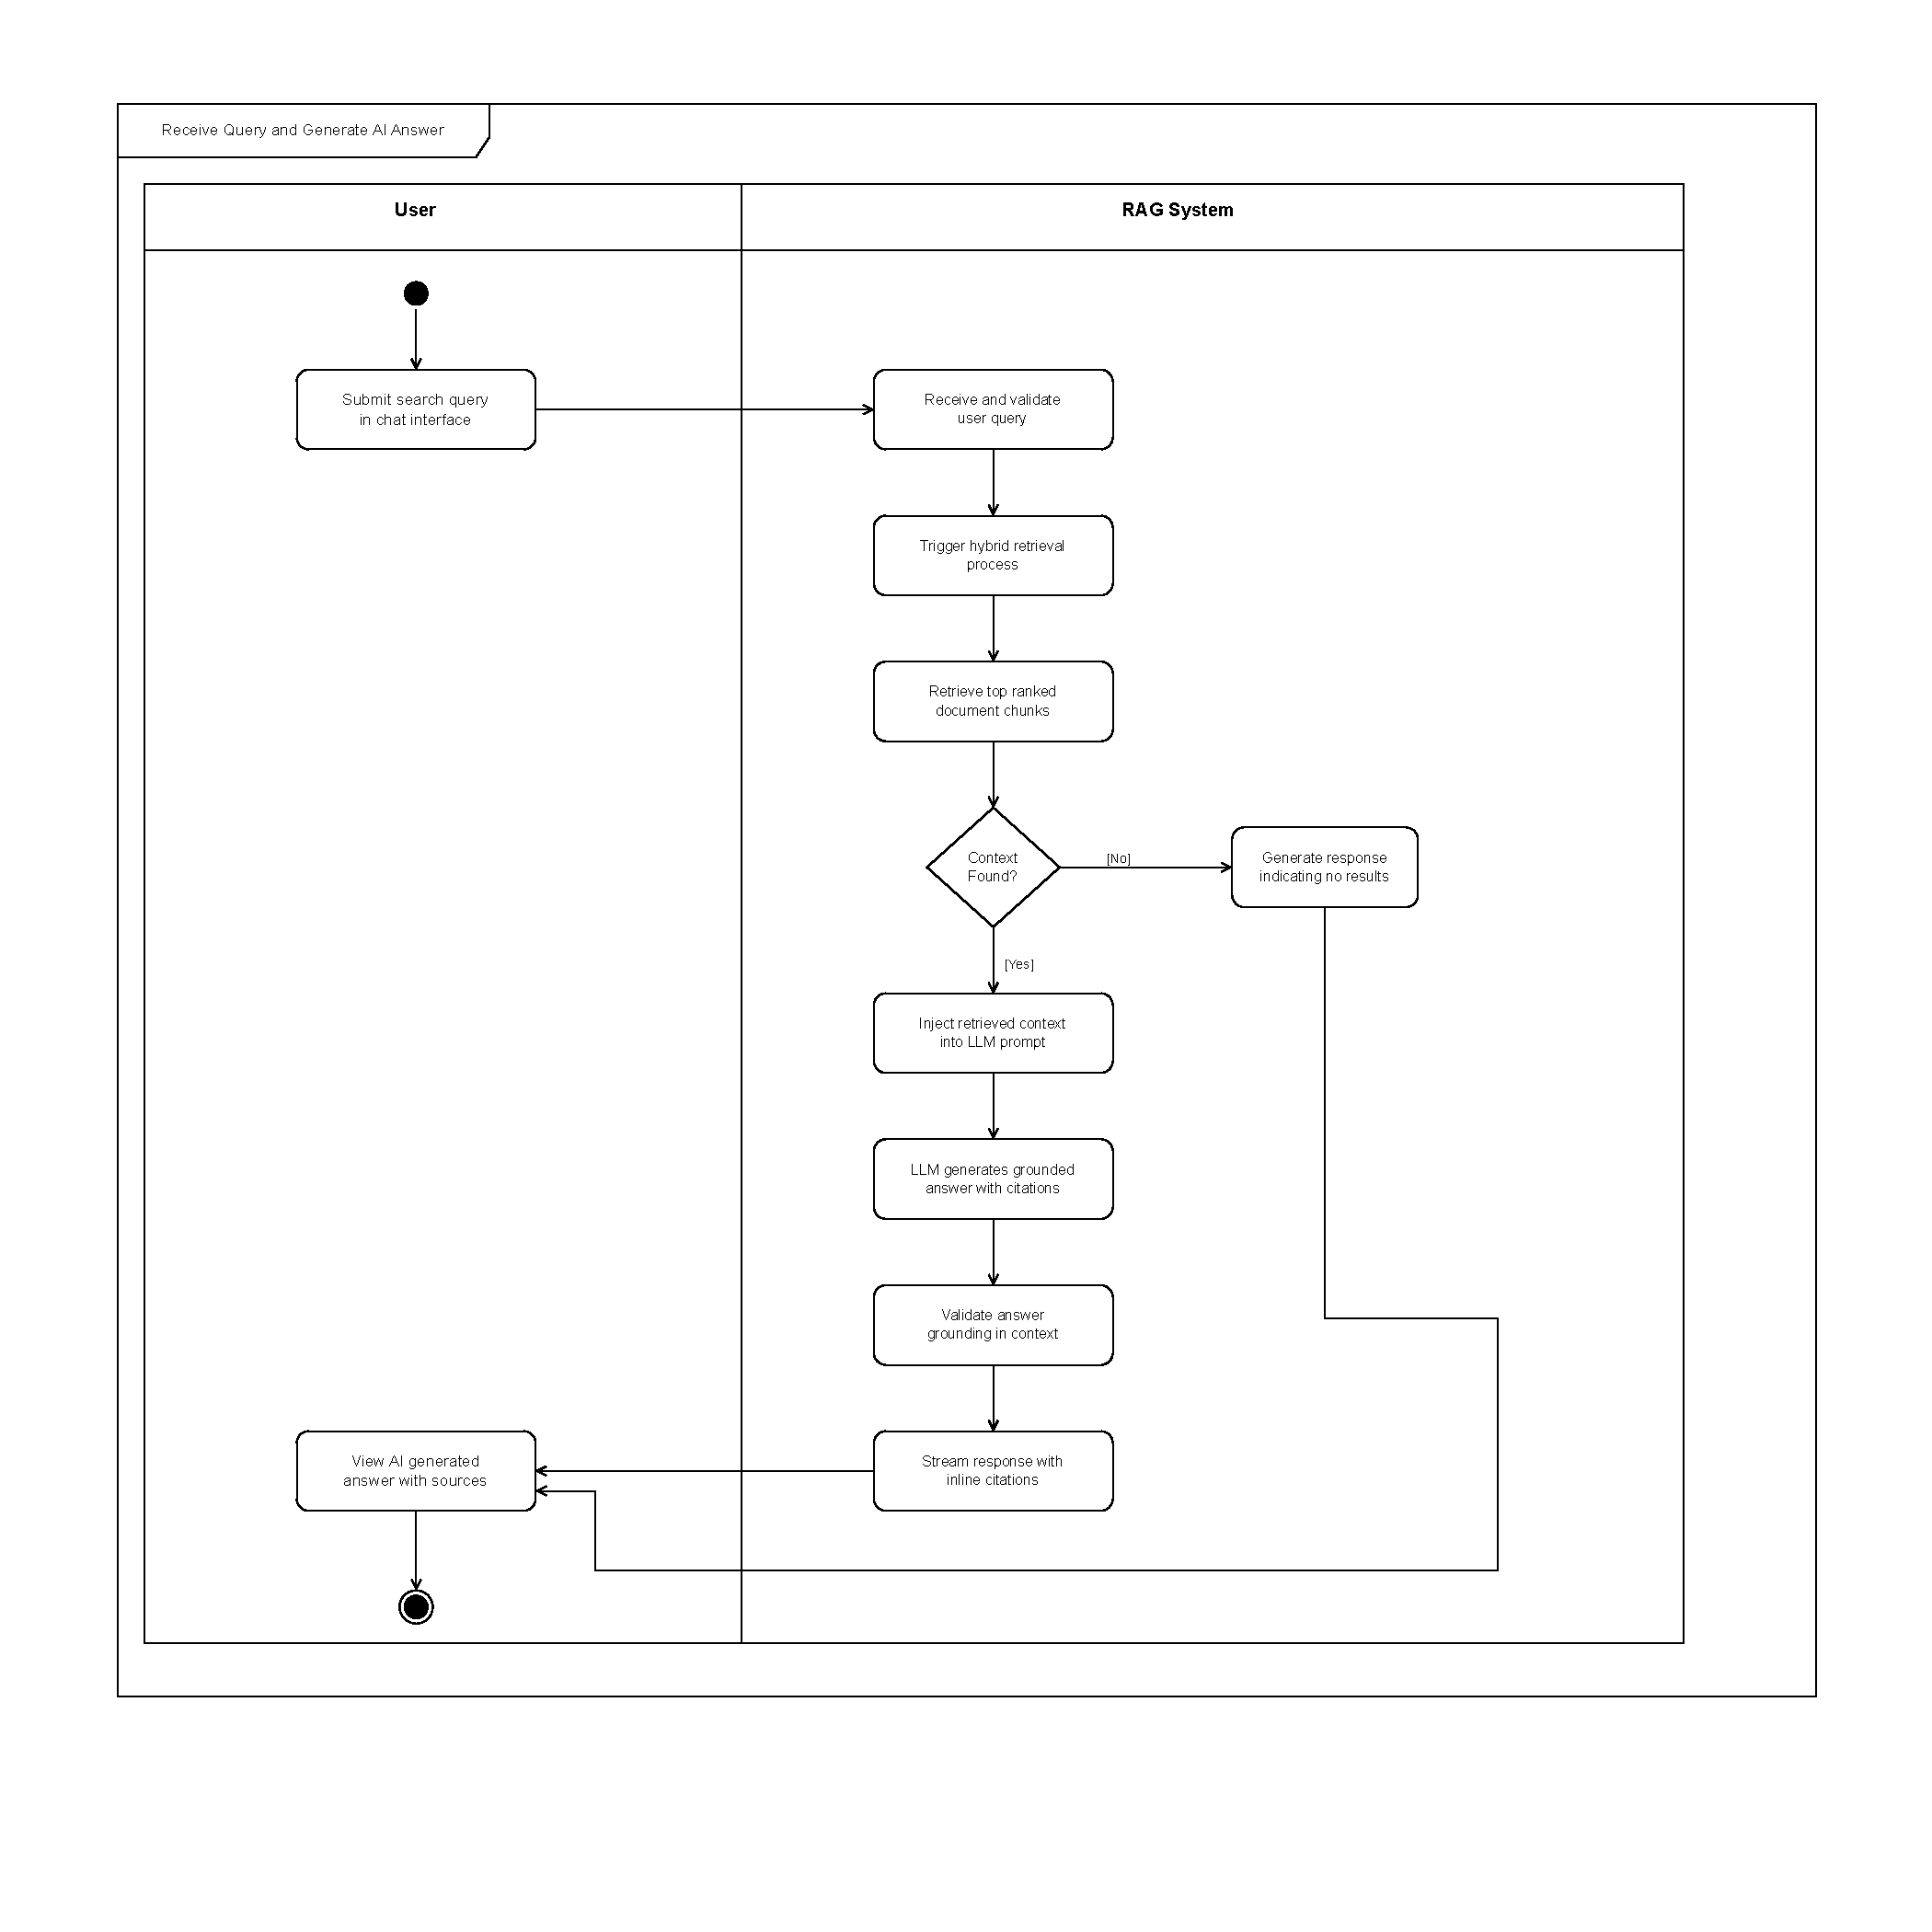
\includegraphics[width=0.55\linewidth]{activity9.drawio.pdf}
    \caption{Activity Diagram: Session Management and Access Control}
    \label{fig:activity9}
\end{figure}

Figure \ref{fig:activity9} details the session management and access control enforcement workflow. Upon successful authentication, the system generates a JWT token containing user ID, roles, and expiration timestamp (24 hours from issuance). This token is stored in a secure HTTP-only cookie to prevent XSS attacks. On each subsequent request, the system validates the JWT signature using the secret key, checks expiration, and extracts user information. When retrieving search results, the system enforces access control by filtering documents based on the user's permissions, querying PostgreSQL for the user's authorized document sets. This ensures users can only access documents they are permitted to view, maintaining data confidentiality across the enterprise.

\begin{figure}[H]
    \centering
    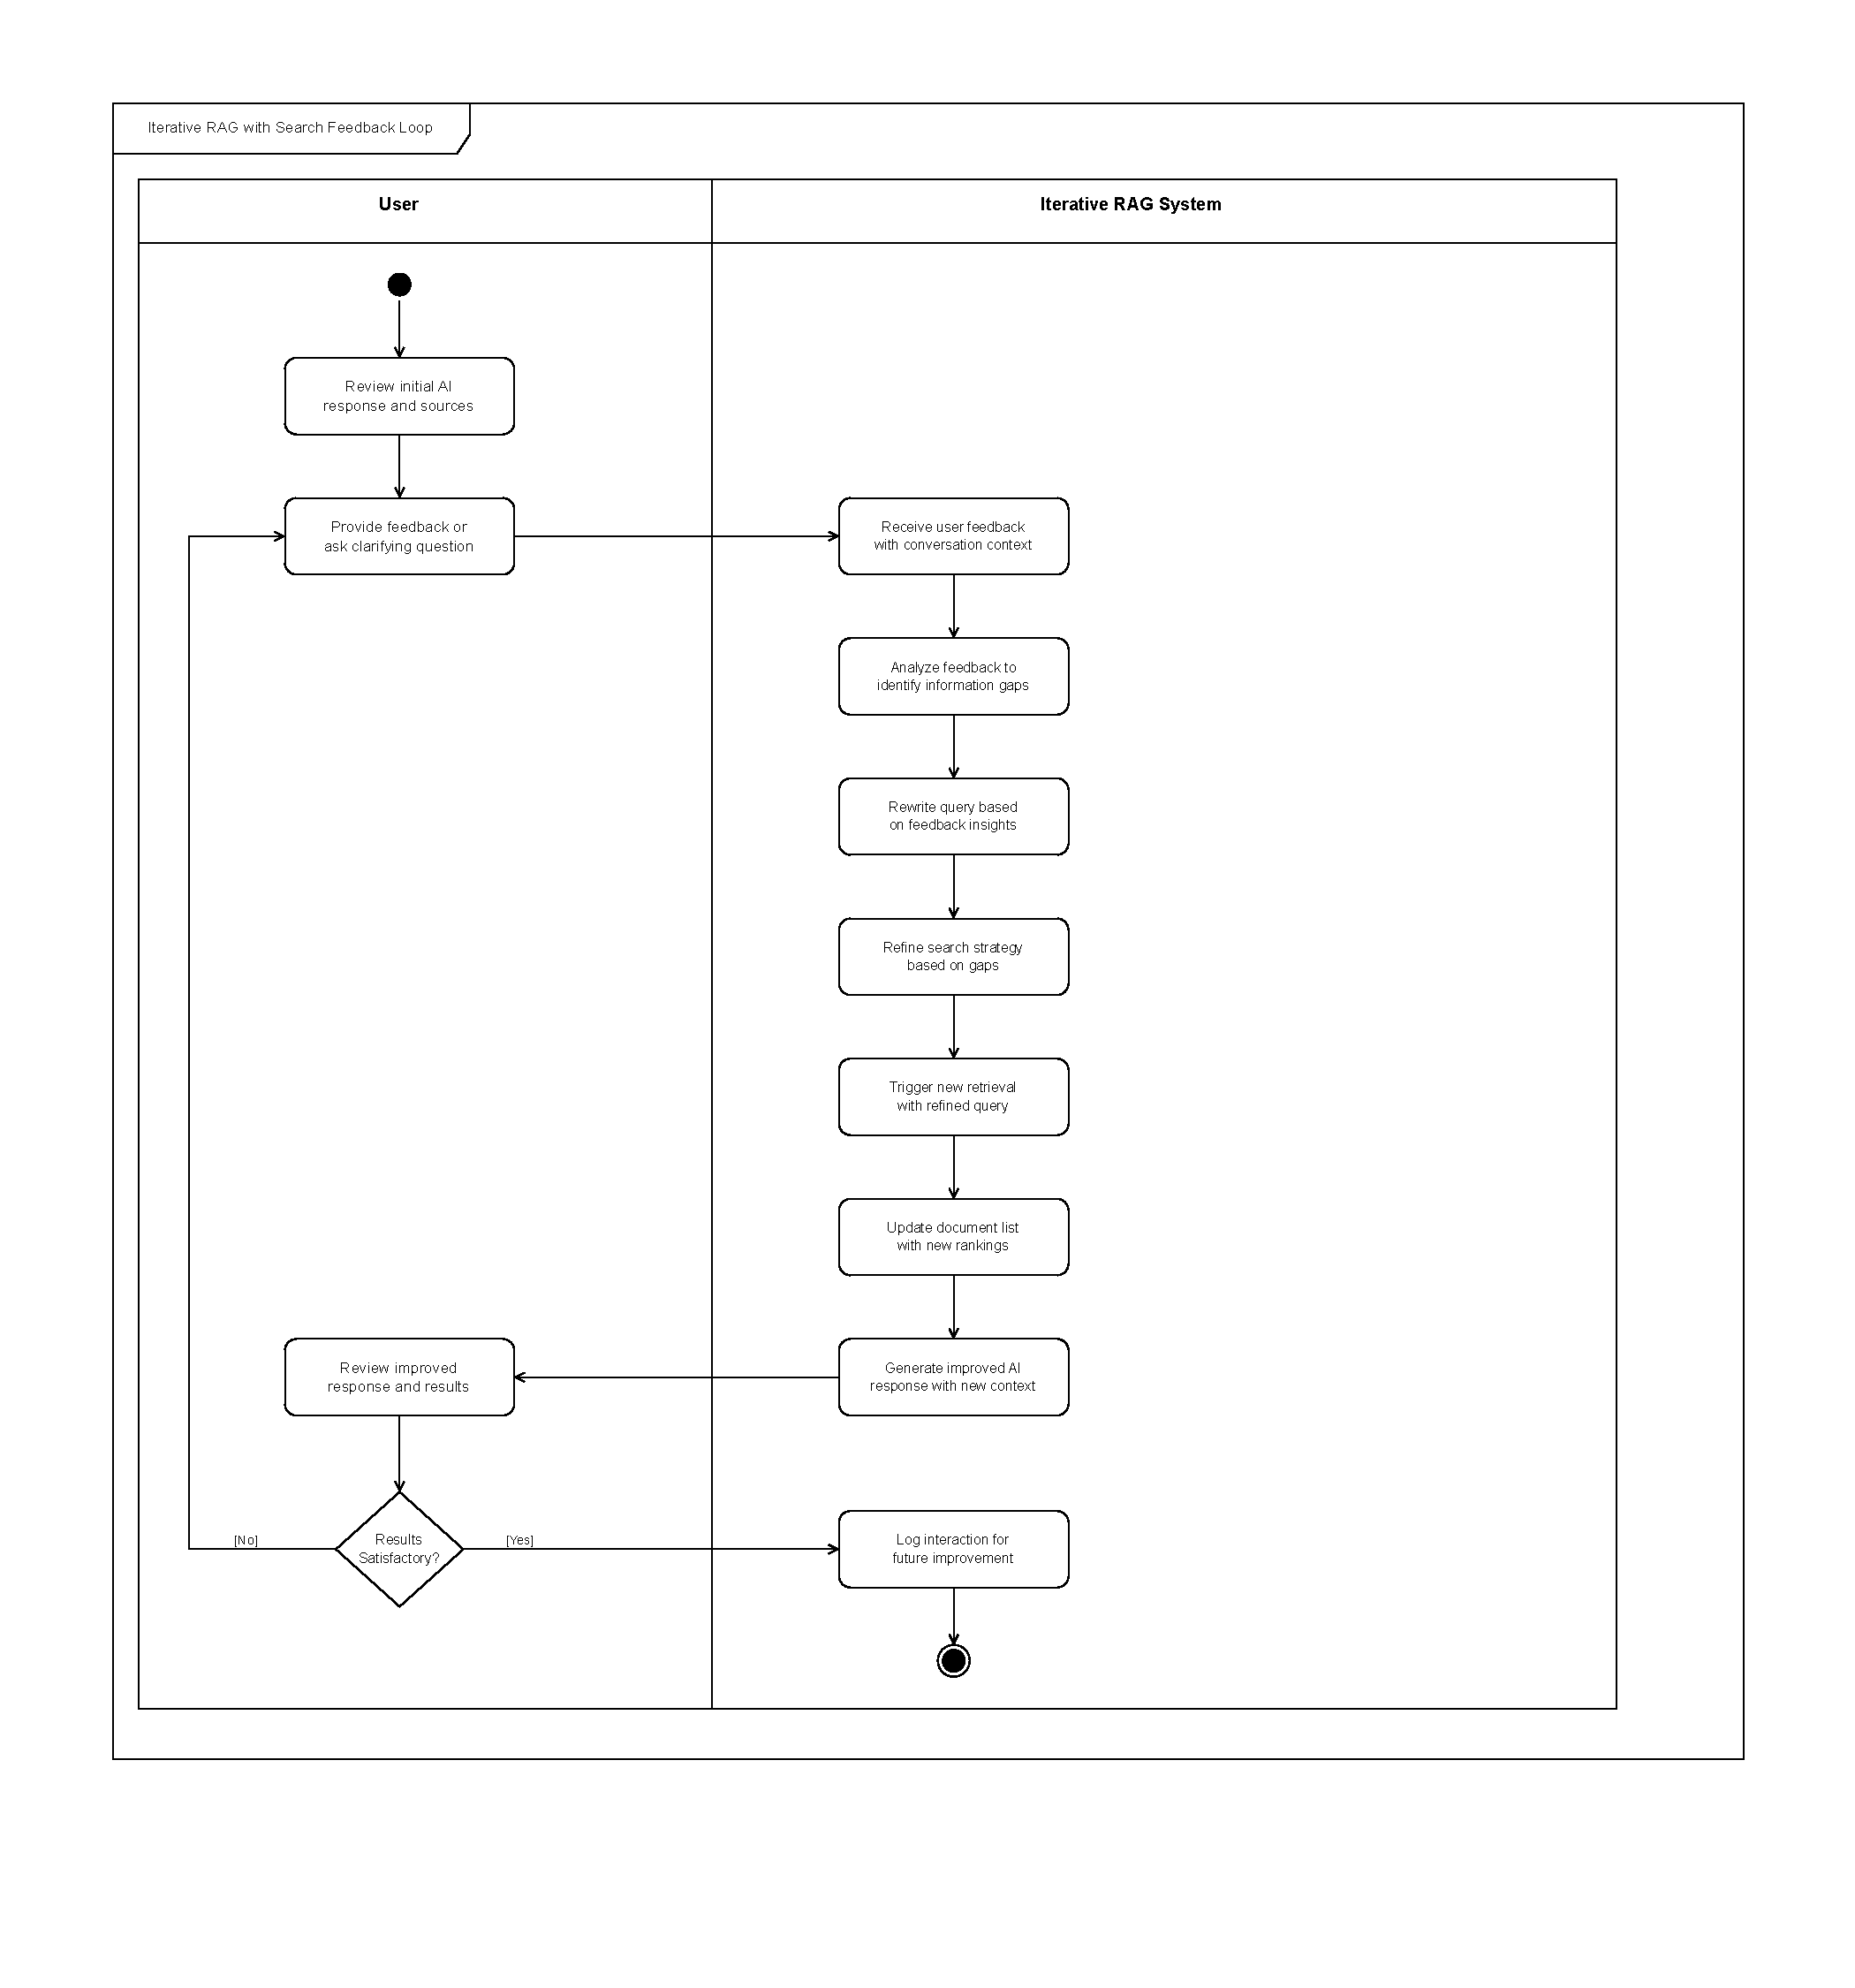
\includegraphics[width=0.55\linewidth]{activity10.drawio.pdf}
    \caption{Activity Diagram: Analytics and Monitoring Workflow}
    \label{fig:activity10}
\end{figure}

Figure \ref{fig:activity10} shows the analytics and monitoring system that tracks search quality and system performance. The system logs each search query with user ID, timestamp, query text, and result count. Query latency is measured at multiple stages (BM25 retrieval, vector search, reranking, total) and exported to Prometheus using histogram metrics. Click-through rates are tracked when users view documents from search results, providing implicit relevance feedback. Grafana dashboards visualize p90/p95/p99 latency distributions, query volume trends, and popular search terms. Alerting rules trigger notifications when latency exceeds 4 seconds or error rates exceed 1\%, enabling proactive performance optimization.

\clearpage


\section{Database Design}

This section presents the database schema for the Verdant Search system, designed using PostgreSQL to store user data, document metadata, search analytics, and system configuration. The database supports efficient query execution while maintaining data integrity through properly normalized tables and carefully designed indexes.

\begin{figure}[H]
    \centering
    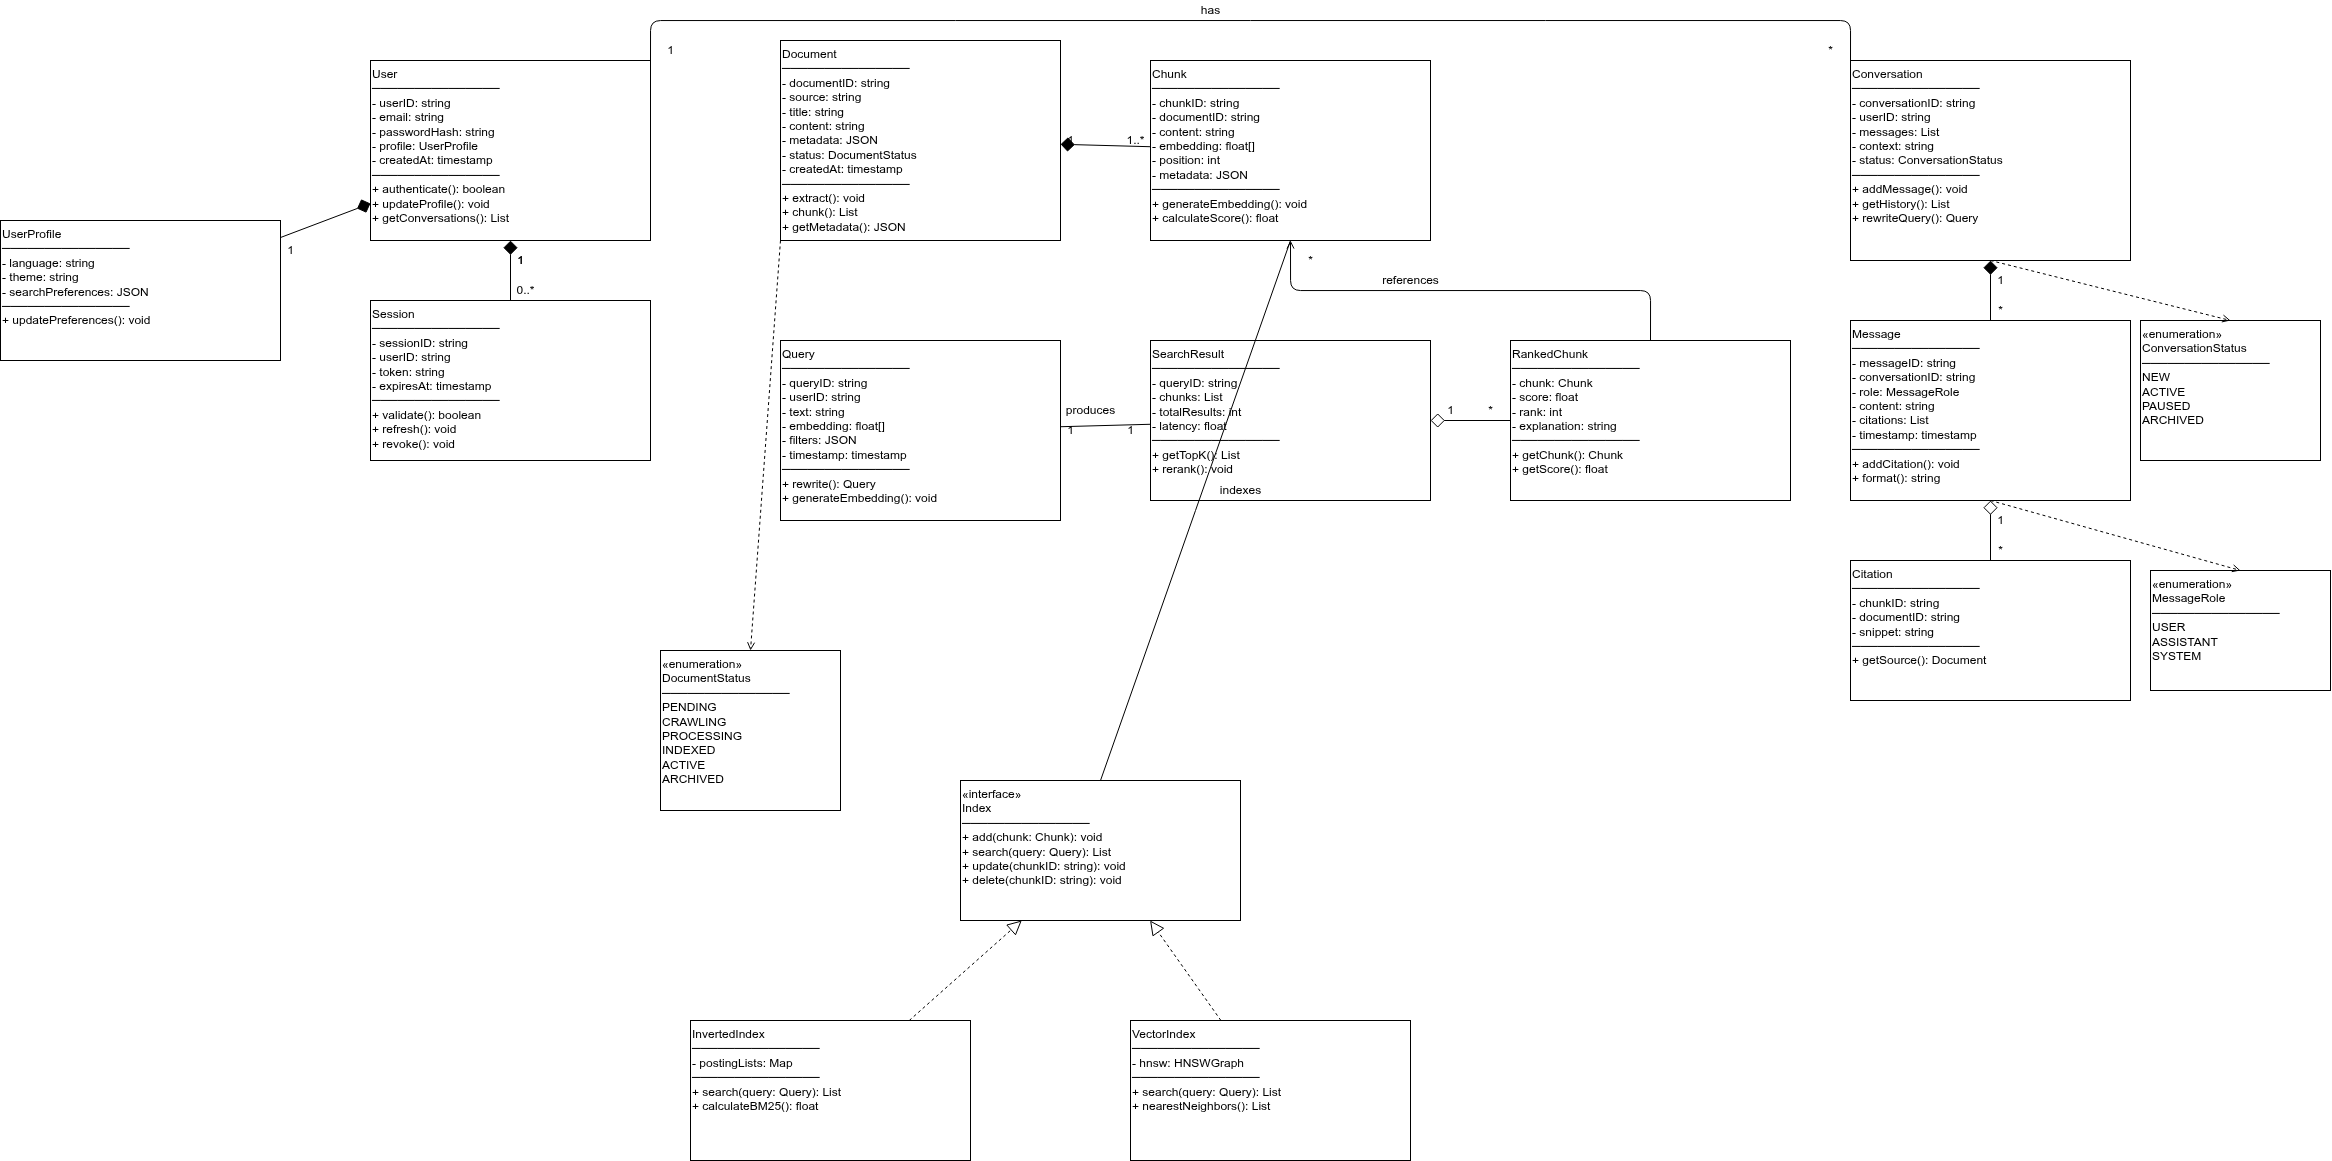
\includegraphics[width=\textwidth]{class.drawio.png}
    \caption{Entity-Relationship Diagram (Class Diagram Format) of Verdant Search Database}
    \label{fig:class_diagram}
\end{figure}

Figure \ref{fig:class_diagram} presents the complete database schema in class diagram notation. The design follows third normal form (3NF) to eliminate data redundancy while optimizing for common query patterns. Key entities and their relationships are described below:

\subsection{User Entity}
The \texttt{User} table stores authentication and profile information. Each user has a unique \texttt{user\_id} (UUID primary key), \texttt{email} (unique index for login lookups), \texttt{password\_hash} (bcrypt with cost factor 12), and optional SSO identifiers (\texttt{sso\_provider}, \texttt{sso\_id}). Profile fields include \texttt{display\_name}, \texttt{avatar\_url}, and \texttt{preferences} (JSONB for flexible settings). Timestamps track account \texttt{created\_at} and \texttt{last\_login}. The email column uses a unique B-tree index to enable fast authentication queries.

\subsection{Session Entity}
The \texttt{Session} table tracks active user sessions with JWT token management. Each session stores the \texttt{session\_id} (UUID), associated \texttt{user\_id} (foreign key to User), \texttt{token\_hash} (SHA-256 hash of JWT for revocation), \texttt{created\_at}, and \texttt{expires\_at} timestamps. An index on \texttt{user\_id} enables efficient retrieval of all sessions for a user. The system periodically purges expired sessions using a background job that deletes rows where \texttt{expires\_at < NOW()}.

\subsection{Document Entity}
The \texttt{Document} table contains metadata for all indexed documents. Core fields include \texttt{document\_id} (UUID), \texttt{title}, \texttt{content\_hash} (SHA-256 for deduplication), \texttt{source\_type} (enum: Confluence, GoogleDrive, Git, NetworkShare), \texttt{source\_url} (original location), \texttt{file\_type} (MIME type), \texttt{file\_size\_bytes}, and storage paths (\texttt{text\_storage\_path}, \texttt{images\_storage\_path}). Timestamps include \texttt{created\_at}, \texttt{modified\_at}, and \texttt{indexed\_at}. A GiN index on \texttt{source\_type} accelerates filtering queries.

\subsection{DocumentChunk Entity}
The \texttt{DocumentChunk} table stores segmented document portions for retrieval. Each chunk has \texttt{chunk\_id} (UUID), parent \texttt{document\_id} (foreign key), \texttt{chunk\_index} (integer position within document), \texttt{text\_content} (up to 2048 characters), \texttt{embedding\_id} (reference to vector index), and \texttt{token\_count}. The compound index on (\texttt{document\_id}, \texttt{chunk\_index}) enables efficient retrieval of all chunks for a document in sequential order.

\subsection{ConversationHistory Entity}
The \texttt{ConversationHistory} table tracks user chat sessions for RAG. Each entry stores \texttt{conversation\_id} (UUID), \texttt{user\_id} (foreign key), \texttt{message\_index} (sequence number), \texttt{role} (enum: user, assistant, system), \texttt{message\_content} (TEXT), and \texttt{timestamp}. An index on (\texttt{user\_id}, \texttt{timestamp} DESC) enables fast retrieval of recent conversation history for query rewriting. The system retains only the last 10 turns per user by periodically deleting older messages.

\subsection{SearchQuery Entity}
The \texttt{SearchQuery} table logs all search queries for analytics. Fields include \texttt{query\_id} (UUID), \texttt{user\_id} (foreign key), \texttt{query\_text}, \texttt{result\_count}, latency metrics (\texttt{bm25\_latency\_ms}, \texttt{vector\_latency\_ms}, \texttt{rerank\_latency\_ms}, \texttt{total\_latency\_ms}), and \texttt{timestamp}. Indexes on \texttt{user\_id} and \texttt{timestamp} support both user-specific query history views and time-series analytics. This table feeds Grafana dashboards for performance monitoring.

\subsection{SearchResult Entity}
The \texttt{SearchResult} table tracks which documents were returned for each query. It links \texttt{query\_id} to \texttt{document\_id} with additional fields for \texttt{rank\_position}, \texttt{relevance\_score}, and \texttt{was\_clicked} (boolean indicating user interaction). This enables click-through rate analysis to measure search quality. The compound index on (\texttt{query\_id}, \texttt{rank\_position}) supports efficient result retrieval.

\subsection{DataSource Entity}
The \texttt{DataSource} table stores configuration for crawl sources. Each source has \texttt{source\_id} (UUID), \texttt{source\_type} (enum matching Document source types), \texttt{connection\_url}, encrypted \texttt{credentials} (AES-256), \texttt{crawl\_schedule} (cron expression), \texttt{last\_crawl\_at}, and \texttt{is\_active} flag. The system decrypts credentials at crawl time using a master key stored in environment variables, never persisting plaintext credentials.

\subsection{CrawlJob Entity}
The \texttt{CrawlJob} table tracks distributed crawling execution. Each job records \texttt{job\_id} (UUID), \texttt{source\_id} (foreign key), \texttt{status} (enum: queued, running, completed, failed), \texttt{started\_at}, \texttt{completed\_at}, progress counters (\texttt{documents\_processed}, \texttt{documents\_failed}), and \texttt{error\_message} if failed. Indexes on \texttt{source\_id} and \texttt{status} enable monitoring dashboard queries.

\subsection{AccessControl Entity}
The \texttt{AccessControl} table implements document permission management. It creates a many-to-many relationship between Users and Documents through entries containing \texttt{user\_id}, \texttt{document\_id}, and \texttt{permission\_level} (enum: read, write, admin). A compound unique index on (\texttt{user\_id}, \texttt{document\_id}) prevents duplicate permission entries. Search queries join this table to filter results based on the requesting user's permissions, enforcing enterprise access control policies.

\subsection{Key Indexes and Performance Optimizations}

The database schema includes carefully designed indexes to support common query patterns:

\begin{itemize}
    \item \textbf{User.email (B-tree unique):} Enables fast login credential lookups with O(log n) complexity.
    \item \textbf{Document.source\_type (GIN):} Accelerates filtering by data source type for source-specific queries.
    \item \textbf{DocumentChunk.(document\_id, chunk\_index) (composite B-tree):} Enables efficient sequential chunk retrieval for RAG context assembly.
    \item \textbf{ConversationHistory.(user\_id, timestamp DESC) (composite B-tree):} Supports fast retrieval of recent conversation history for query rewriting.
    \item \textbf{SearchQuery.timestamp (B-tree):} Enables time-series analytics queries for Grafana dashboards.
    \item \textbf{AccessControl.(user\_id, document\_id) (unique composite):} Ensures unique permissions and accelerates access control checks during search.
\end{itemize}

All tables use UUID primary keys to enable distributed database scaling and prevent ID collision. Foreign key constraints enforce referential integrity, with CASCADE deletes configured where appropriate (e.g., deleting a User cascades to their Sessions and ConversationHistory).

\clearpage


\section{Deployment Architecture}

\begin{figure}[H]
    \centering
    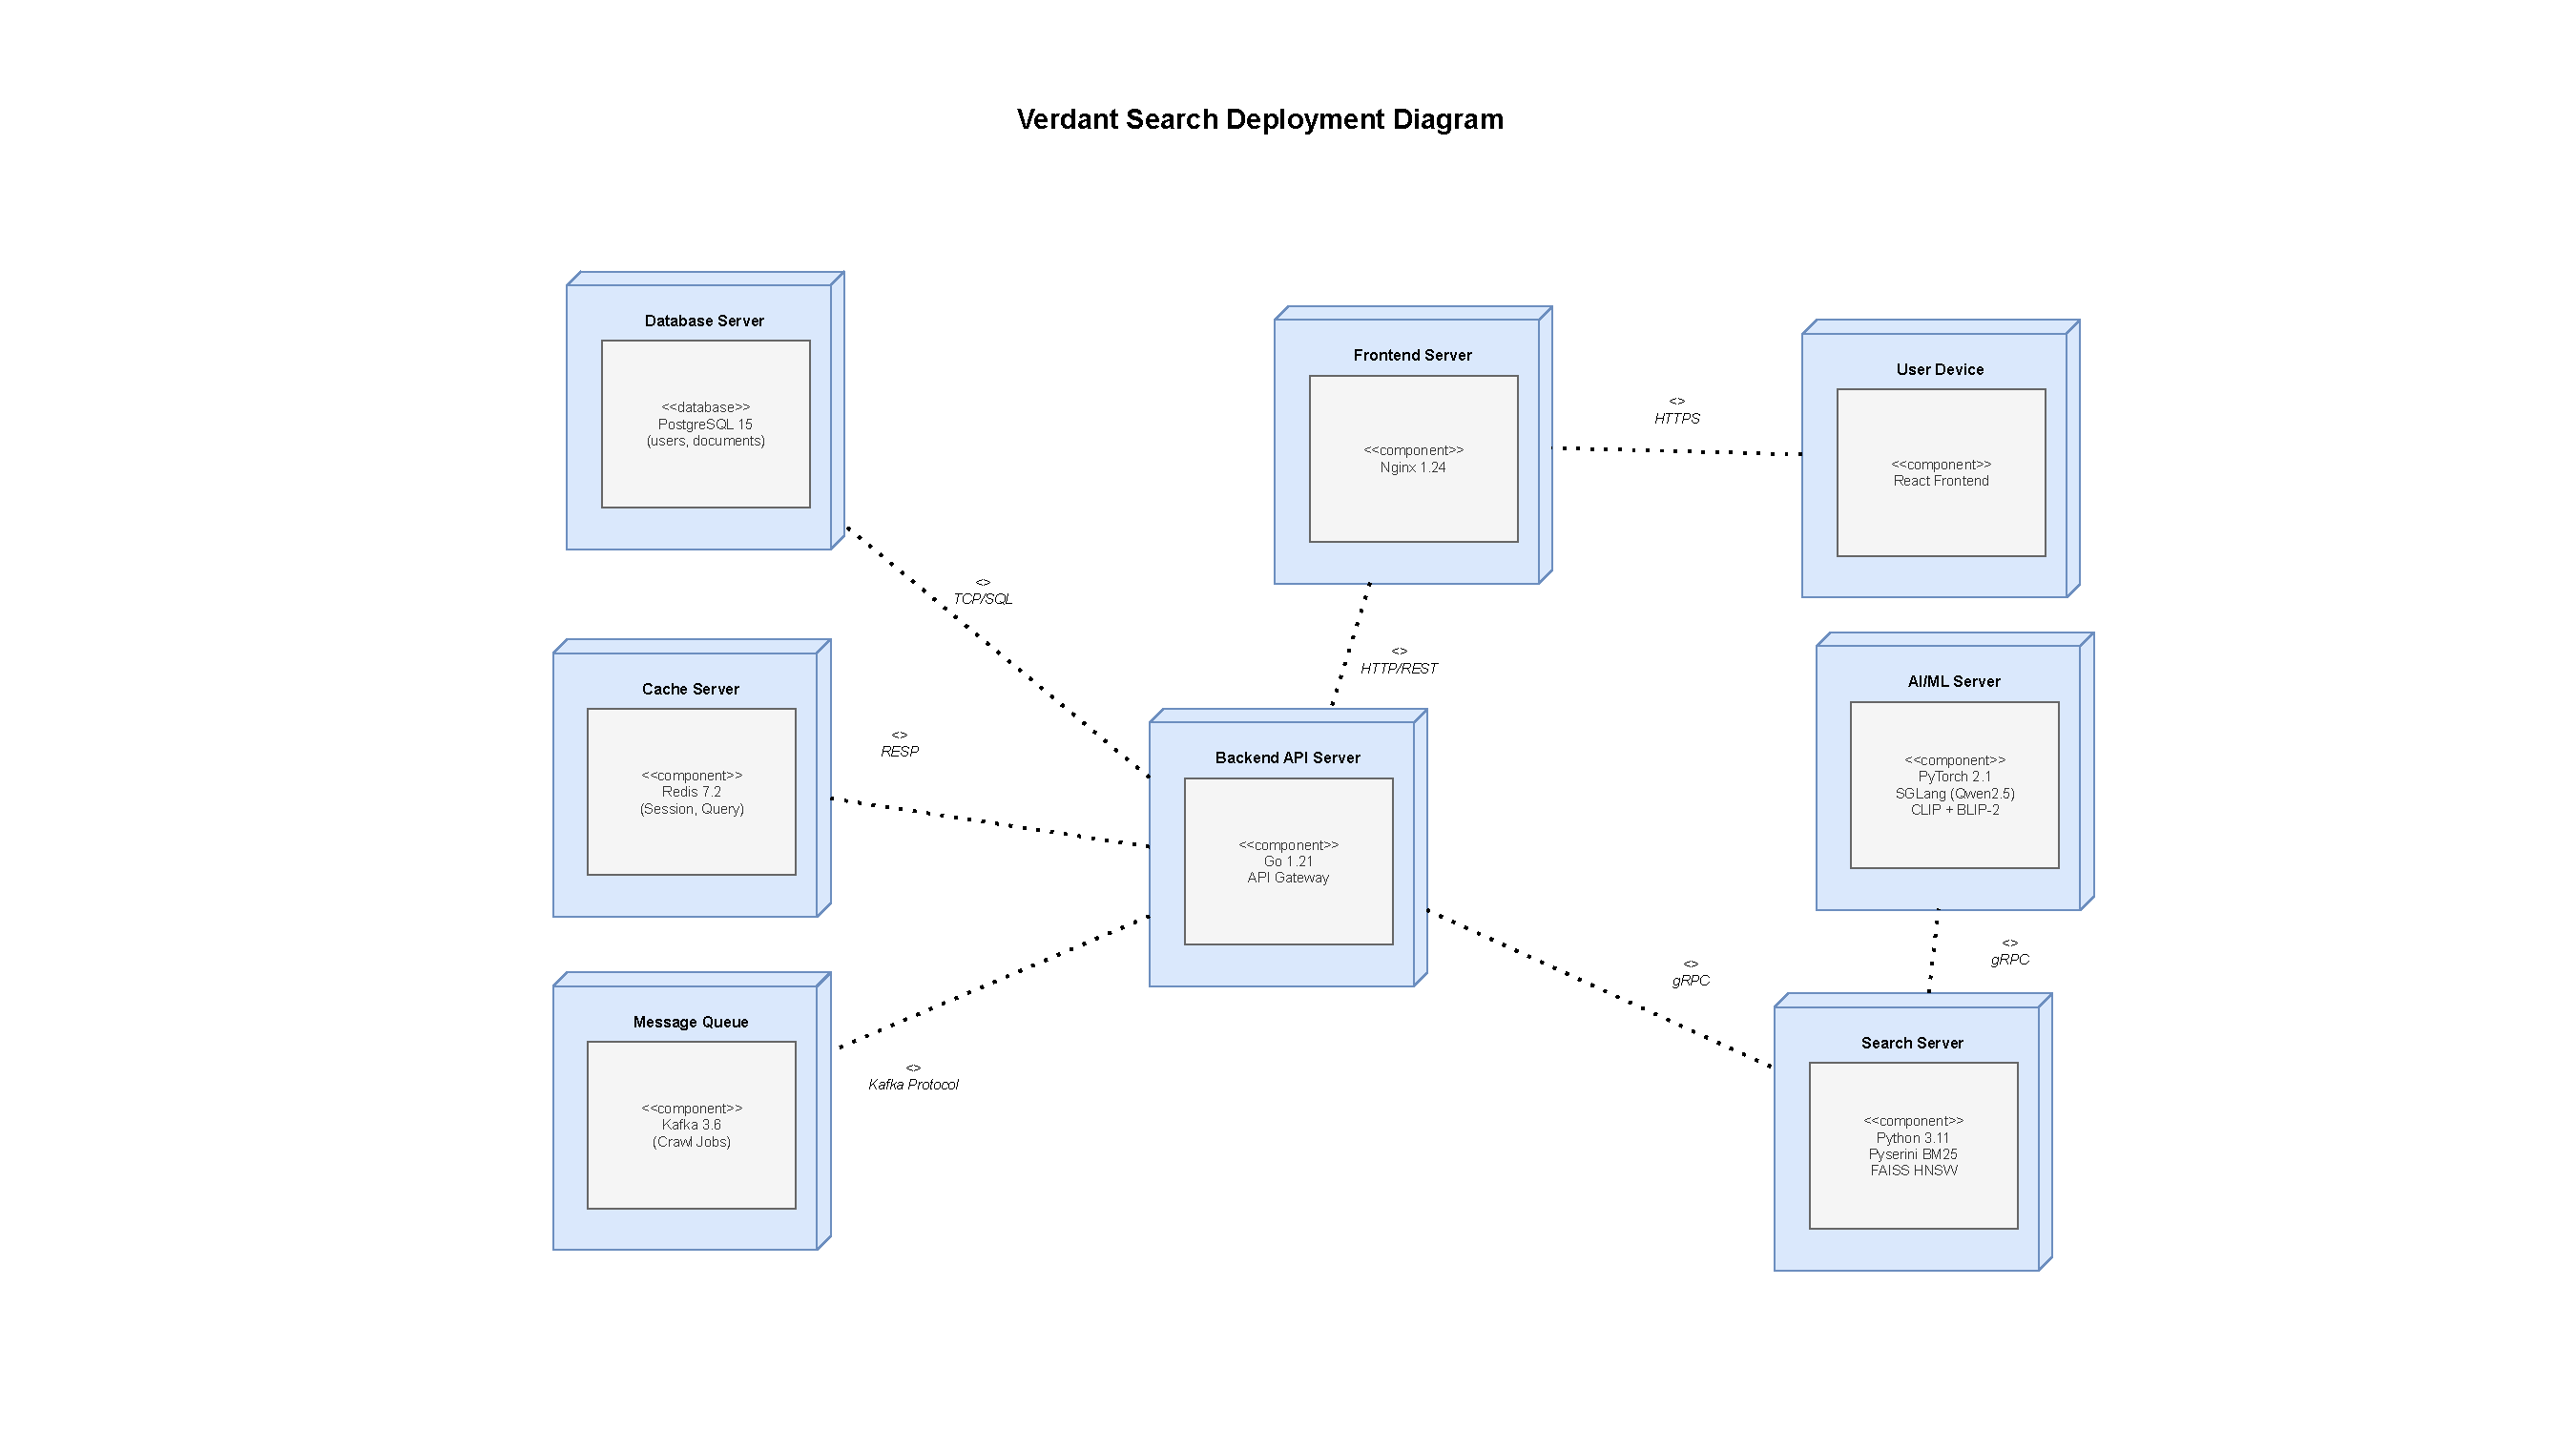
\includegraphics[width=\textwidth]{deployment.drawio.pdf}
    \caption{Deployment Diagram of Verdant Search System}
    \label{fig:deployment}
\end{figure}

Figure \ref{fig:deployment} illustrates the deployment architecture of the Verdant Search platform across development and production environments. The system employs a microservices architecture deployed using Docker containers orchestrated by Kubernetes for scalability and fault tolerance.

\subsection{Client Tier}
User browsers access the system through HTTPS, connecting to the load balancer which distributes requests across multiple frontend pods. The React-based single-page application is served from an Nginx container, with TailwindCSS providing responsive styling and Shadcn components ensuring accessible UI elements. Static assets are cached using CDN for global low-latency access.

\subsection{Application Tier}
The application tier consists of several microservices:

\begin{itemize}
    \item \textbf{API Gateway (Kong):} Handles authentication, rate limiting, and request routing to backend services.
    \item \textbf{Search Service (Golang):} Executes BM25 and vector search, coordinates hybrid fusion, and triggers multimodal reranking.
    \item \textbf{Ingestion Service (Golang):} Coordinates distributed crawling via Kafka, processes documents, and manages index building.
    \item \textbf{RAG Service (Python/FastAPI):} Handles context injection, LLM inference via SGLang, and answer streaming.
    \item \textbf{Analytics Service (Golang):} Collects metrics and exports to Prometheus for monitoring.
\end{itemize}

Each service runs in multiple pods behind a Kubernetes Service for load balancing and automatic failover.

\subsection{Data Tier}
The data layer includes:

\begin{itemize}
    \item \textbf{PostgreSQL (Primary + Replica):} Stores user data, document metadata, and search analytics with streaming replication for high availability.
    \item \textbf{Redis Cluster:} Provides session storage, conversation history caching, and query result caching with automatic sharding.
    \item \textbf{Kafka Cluster:} Coordinates distributed crawling and document processing with 3 broker nodes for fault tolerance.
    \item \textbf{Object Storage (MinIO):} Stores document content, extracted images, and index snapshots with S3-compatible API.
\end{itemize}

\subsection{ML Infrastructure}
\begin{itemize}
    \item \textbf{FAISS Index Servers:} Serve HNSW vector indices loaded in memory for fast ANN search, deployed on nodes with sufficient RAM (32GB+).
    \item \textbf{Pyserini Index Servers:} Serve BM25 inverted indices with Lucene backend for keyword retrieval.
    \item \textbf{SGLang Inference Cluster:} Hosts LLM models on GPU nodes (NVIDIA RTX 5090) for RAG answer generation and query rewriting.
    \item \textbf{BLIP-2 Reranker Service:} Runs multimodal reranking on GPU nodes, processing top-K candidates from hybrid search.
\end{itemize}

\subsection{Monitoring and Observability}
\begin{itemize}
    \item \textbf{Prometheus:} Scrapes metrics from all services at 15-second intervals, retaining 30 days of data.
    \item \textbf{Grafana:} Visualizes metrics dashboards for query latency, system health, and search quality indicators.
    \item \textbf{ELK Stack (Elasticsearch, Logstash, Kibana):} Aggregates logs from all microservices for centralized debugging and audit trail analysis.
\end{itemize}

\subsection{Development Environment}
The development environment uses the same containerized architecture with Docker Compose for local testing. Key differences include single-node deployments without replication, and reduced resource allocations to fit development hardware (16GB RAM, NVIDIA RTX 2080 Ti GPU).

\clearpage

\section{Non-Functional Requirements}

This section specifies the quality attributes that the Verdant Search system must satisfy to meet Infinity Datatech's enterprise deployment standards.

\begin{table}[H]
\centering
\caption{Non-Functional Requirements Specification}
\label{tab:nfr}
\small
\renewcommand{\arraystretch}{1.4}
\begin{tabularx}{\textwidth}{|p{0.08\textwidth}|p{0.15\textwidth}|p{0.30\textwidth}|p{0.20\textwidth}|p{0.15\textwidth}|}
\hline
\textbf{Req ID} & \textbf{Quality Attribute} & \textbf{Requirement Description} & \textbf{How to Achieve} & \textbf{How to Verify} \\
\hline
NFR-1.1 & Security: Authenticity & System shall integrate with Infinity Datatech's internal identity providers for centralized authentication. & LDAP/SAML/OAuth2 integration with JWT token-based sessions & SSO login testing with enterprise credentials \\
\hline
NFR-1.2 & Security: Confidentiality & Search results shall respect document access permissions; users can only retrieve documents they are authorized to view. & ACL enforcement during retrieval by joining AccessControl table & Access audit logs showing denied access attempts \\
\hline
NFR-1.3 & Security: Data Privacy & All data shall be stored in Infinity Datatech's private infrastructure; LLM models shall be self-hosted to prevent data leakage. & On-premise deployment with AES-256 encryption at rest and in transit & Security audit confirming no external API calls with sensitive data \\
\hline
NFR-2.1 & Performance: Latency & P90 latency from query submission to complete ranked results shall be under 4 seconds. & Two-stage ranking (fast retrieval + bounded reranking) with Redis caching & Prometheus monitoring showing p90 latency metrics \\
\hline
NFR-2.2 & Performance: Scalability & System shall scale to index and search 10 million documents without degradation. & Distributed HNSW sharding via FAISS + Kafka-coordinated crawling & Load testing with 10M document corpus measuring throughput \\
\hline
NFR-3.1 & Reliability: Fault Tolerance & System shall implement comprehensive error handling, automatic retries, and graceful degradation. & Circuit breakers for service calls + exponential backoff retries + centralized logging via ELK & Chaos engineering tests (random pod termination) \\
\hline
NFR-4.1 & Maintainability: Modularity & System components shall be independently deployable and upgradable without full system restart. & Microservices architecture + Docker containers + Kubernetes orchestration & Zero-downtime deployment tests using rolling updates \\
\hline
NFR-5.1 & Usability: Learnability & New users shall be able to perform basic search and understand results within 5 minutes without training. & Intuitive dual-panel UI + inline help tooltips + example queries & User testing sessions (n=10 employees) measuring time-to-first-successful-search \\
\hline
\end{tabularx}
\end{table}

\subsection{Security Requirements Detail}
The system implements defense-in-depth with multiple security layers: JWT tokens with short expiration (24h) prevent session hijacking; bcrypt password hashing with cost factor 12 protects credentials; HTTPS with TLS 1.3 encrypts all network traffic; document access control checks occur at retrieval time, preventing unauthorized access; and audit logging tracks all authentication events and search queries for forensic analysis.

\subsection{Performance Requirements Detail}
To achieve sub-4-second P90 latency, the architecture employs several optimizations: parallel execution of BM25 and vector search reduces latency by 40\%; Redis caching of frequent queries provides instant responses for cache hits (20\% of queries); multimodal reranking is applied only to top-20 candidates, bounding expensive GPU inference; and query result pagination limits initial payload size, enabling progressive loading of detailed results.

\subsection{Scalability Approach}
Horizontal scalability is achieved through stateless microservices that can be replicated across Kubernetes nodes. FAISS HNSW indices are sharded by document ID ranges, with each shard served by dedicated pods. PostgreSQL read replicas distribute analytics queries. Kafka partitions enable parallel crawling across worker nodes. This architecture supports linear scaling by adding nodes as document count grows.

\clearpage

\section{User Interface Design}

The Verdant Search user interface is designed following modern web design principles, emphasizing usability, accessibility, and visual clarity. The interface implements a dual-panel layout that seamlessly integrates traditional document search with conversational AI-powered question answering, providing users with flexible interaction modes suited to different information-seeking tasks.

\subsection{Design Philosophy}

The UI design prioritizes three core principles: (1) \textbf{Progressive Disclosure} - presenting information hierarchically to avoid overwhelming users while maintaining access to advanced features; (2) \textbf{Contextual Awareness} - adapting the interface based on user actions and search context; and (3) \textbf{Visual Feedback} - providing immediate, clear feedback for all user interactions through loading states, animations, and status indicators.

\begin{figure}[H]
    \centering
    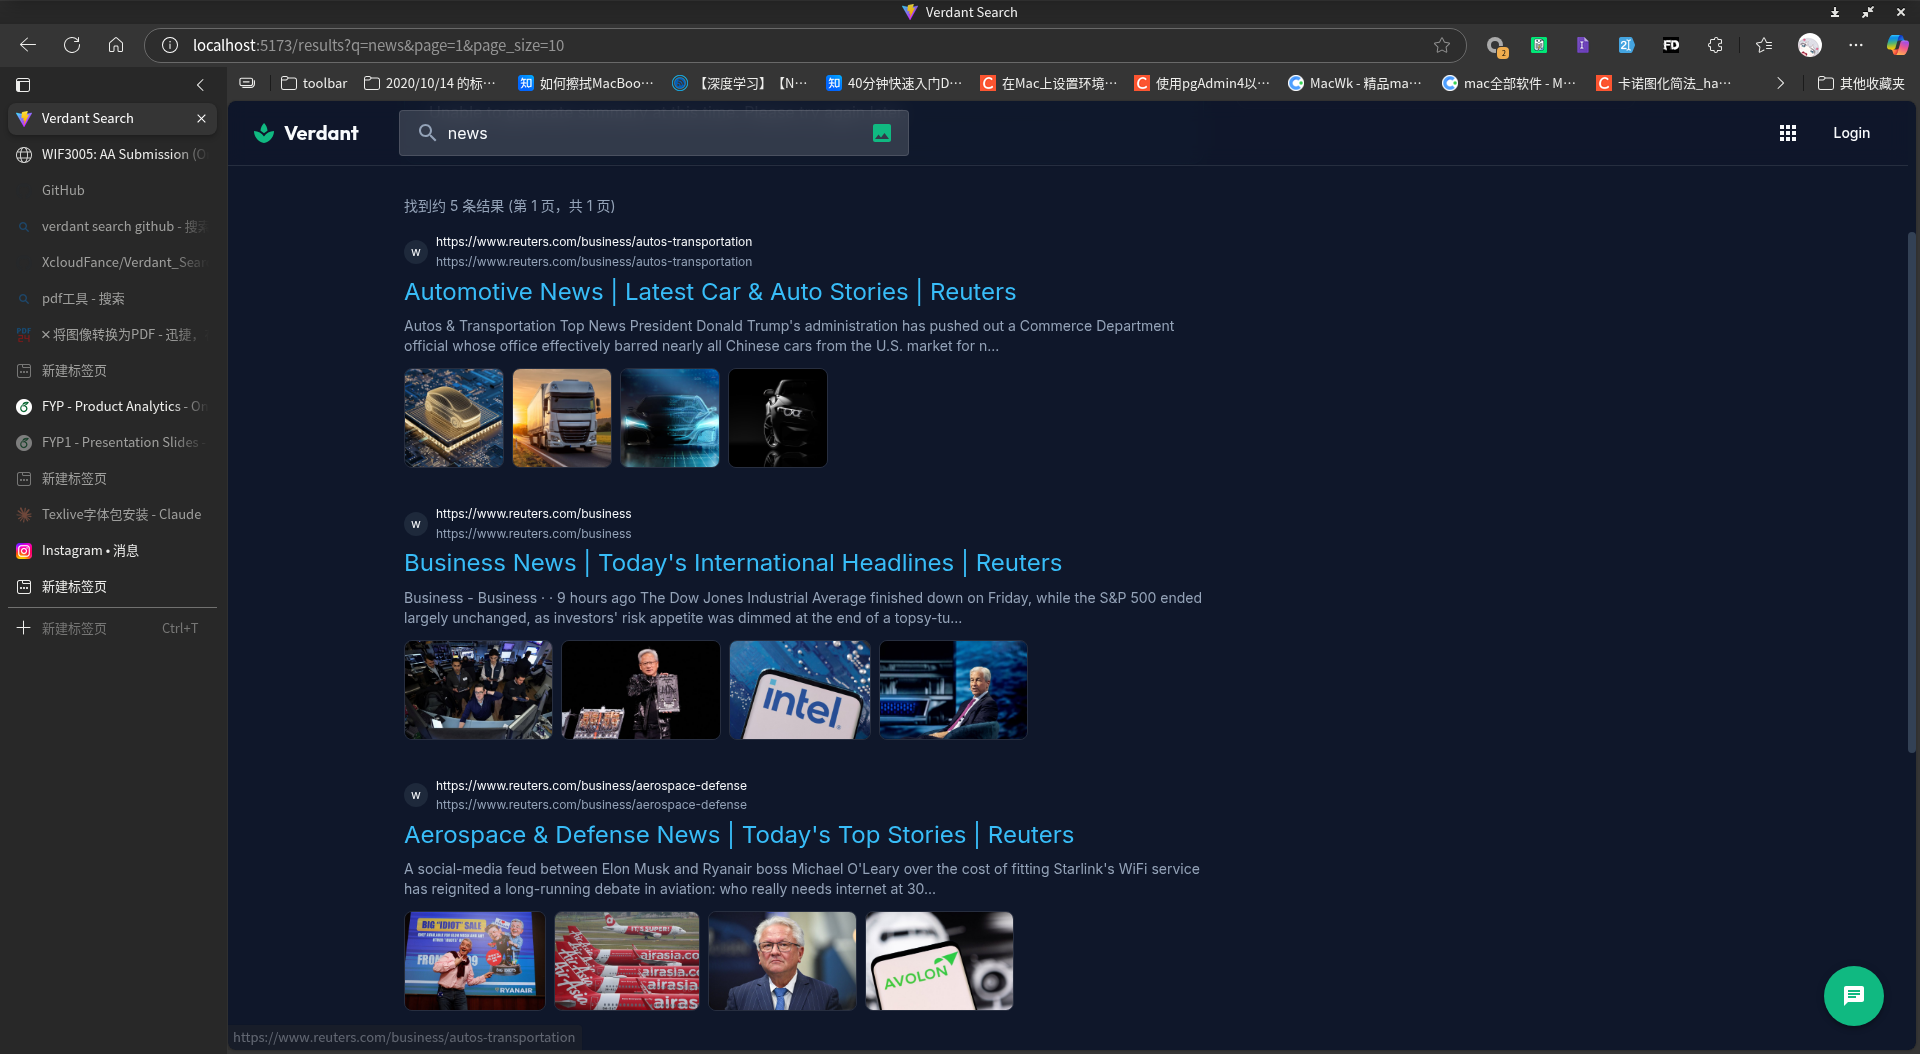
\includegraphics[width=0.95\linewidth]{screenshot1.png}
    \caption{Landing Page and Initial Search Interface}
    \label{fig:ui0}
\end{figure}

Figure \ref{fig:ui0} presents the landing page that users encounter upon accessing Verdant Search. The clean, minimalist design features a prominent search bar centered on the page, inviting users to begin their search journey. The interface includes quick-start examples showing common query patterns ("Find documentation about...", "How do I configure..."), helping new users understand the system's capabilities. The top navigation bar provides access to user profile settings, search history, and system documentation. The color scheme uses Infinity Datatech's corporate palette with subtle gradients and shadows to create visual depth while maintaining professional aesthetics.

\begin{figure}[H]
    \centering
    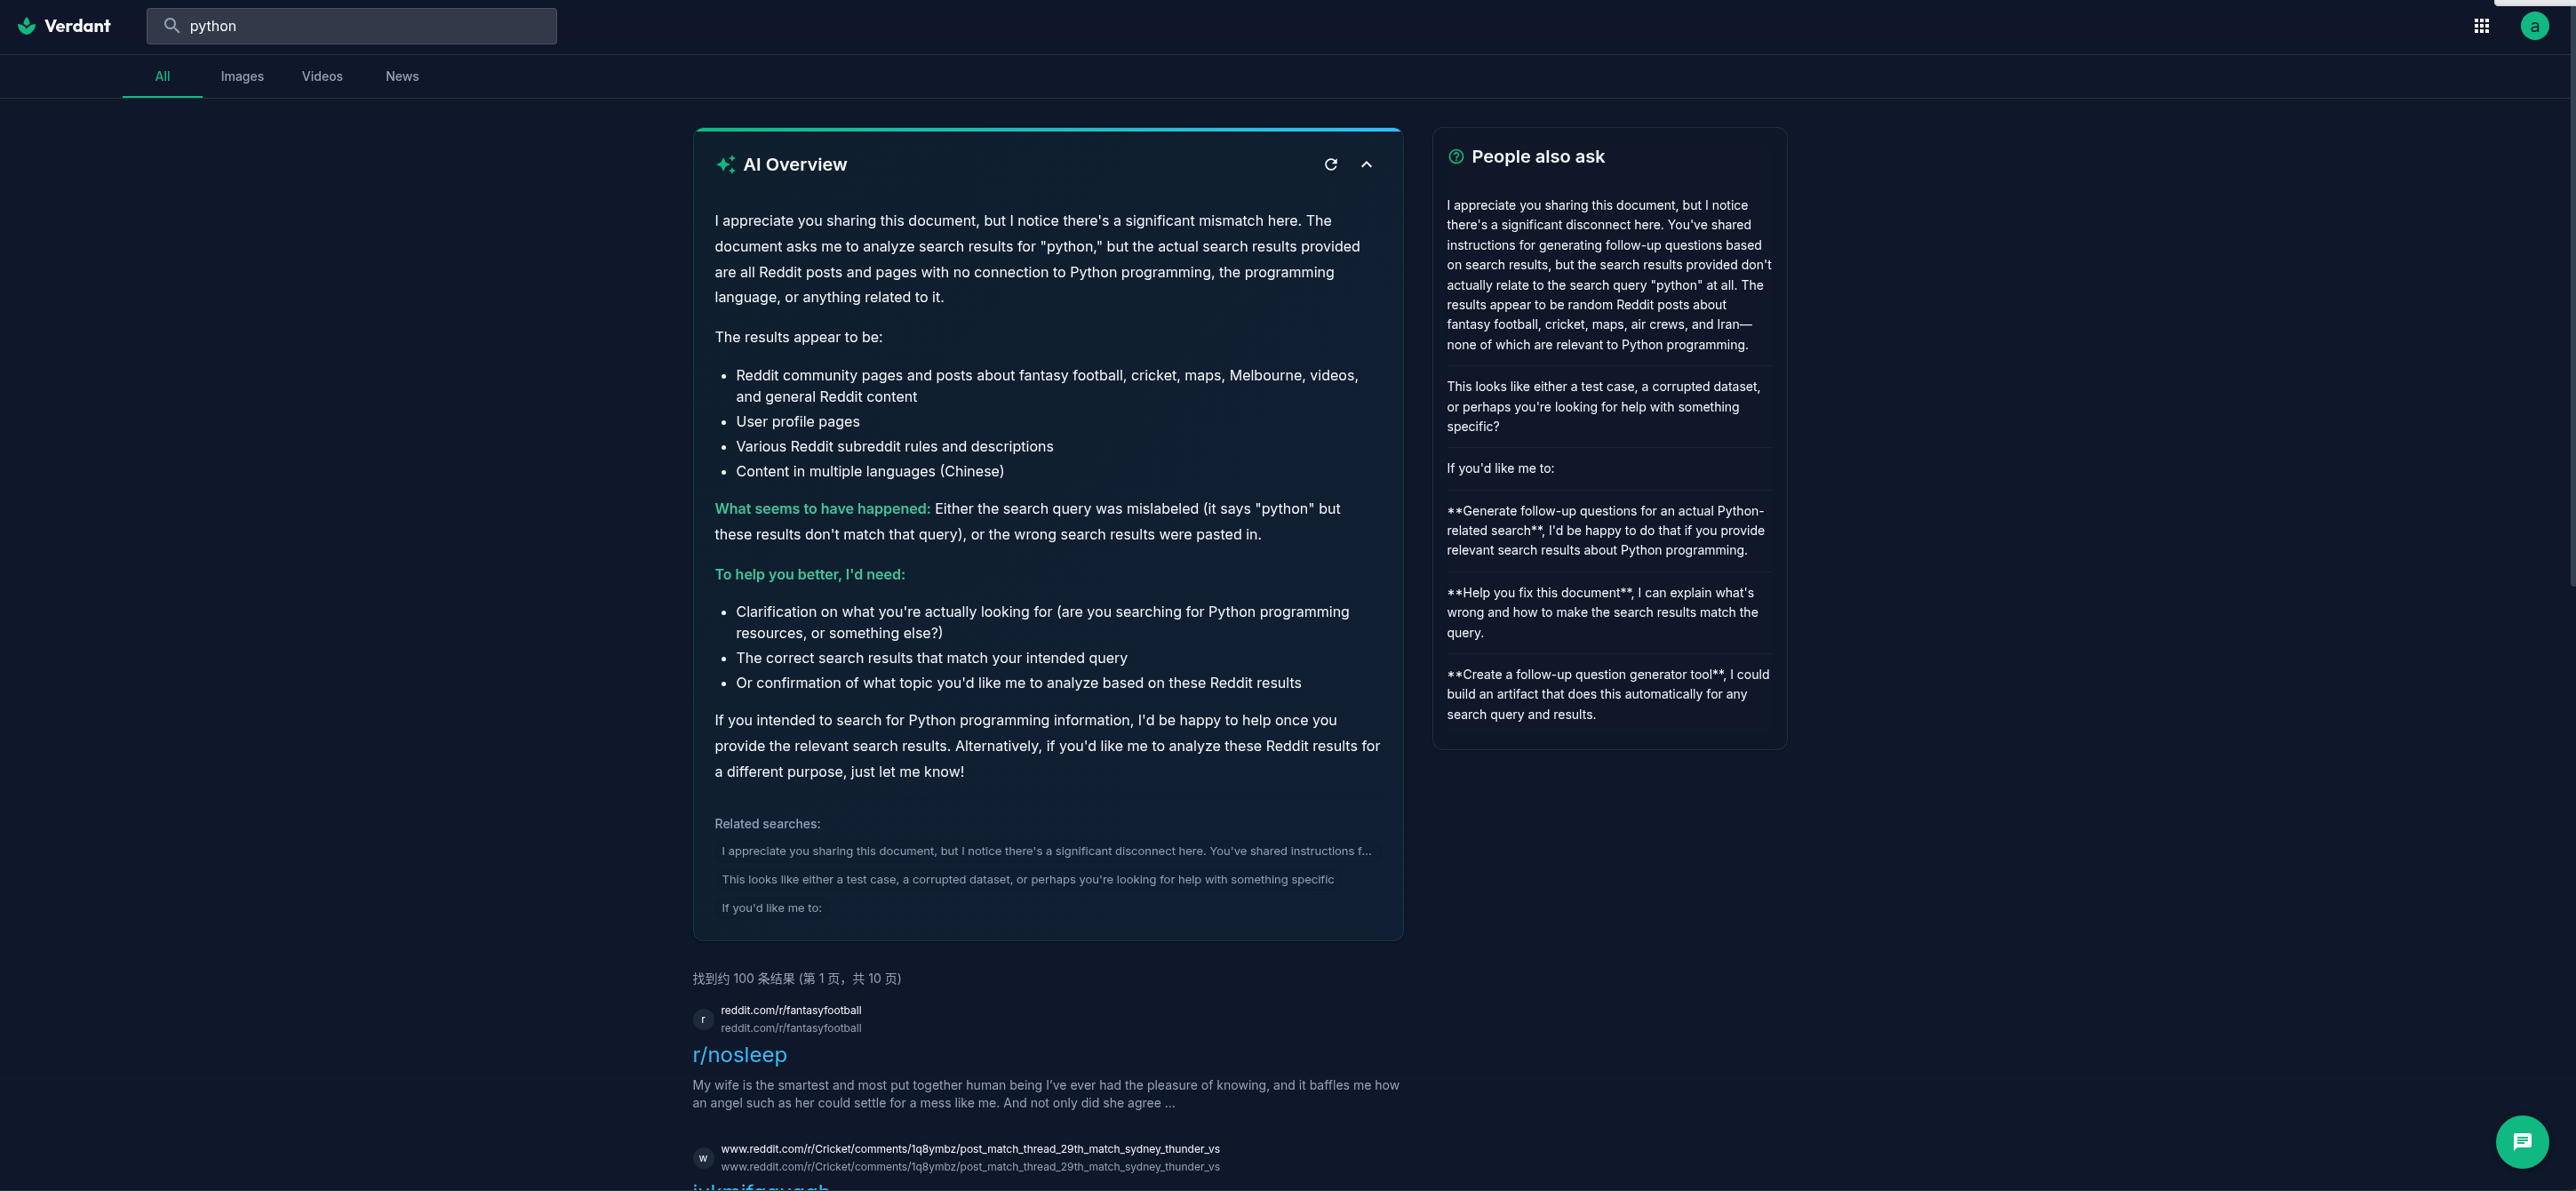
\includegraphics[width=0.95\linewidth]{ui_screenshot_1.png}
    \caption{Main Search Interface with Dual Panel Layout}
    \label{fig:ui1}
\end{figure}

Figure \ref{fig:ui1} shows the main search interface activated after a user submits a query. The interface transitions to a dual-panel layout optimized for information exploration. The left panel displays the ranked document list, with each result card showing: (1) document title as a clickable link, (2) relevant text snippet with query keywords highlighted in yellow, (3) multimodal relevance score visualized as a progress bar, (4) source metadata including filename, document type icon, and last modified timestamp, and (5) thumbnail previews of embedded images when available. Users can filter results using faceted search controls at the top (document type, date range, source system). The right panel contains the RAG chat interface, initially collapsed but expandable with a single click. This design enables seamless switching between traditional search (browsing documents) and conversational search (asking specific questions about the retrieved content).

\begin{figure}[H]
    \centering
    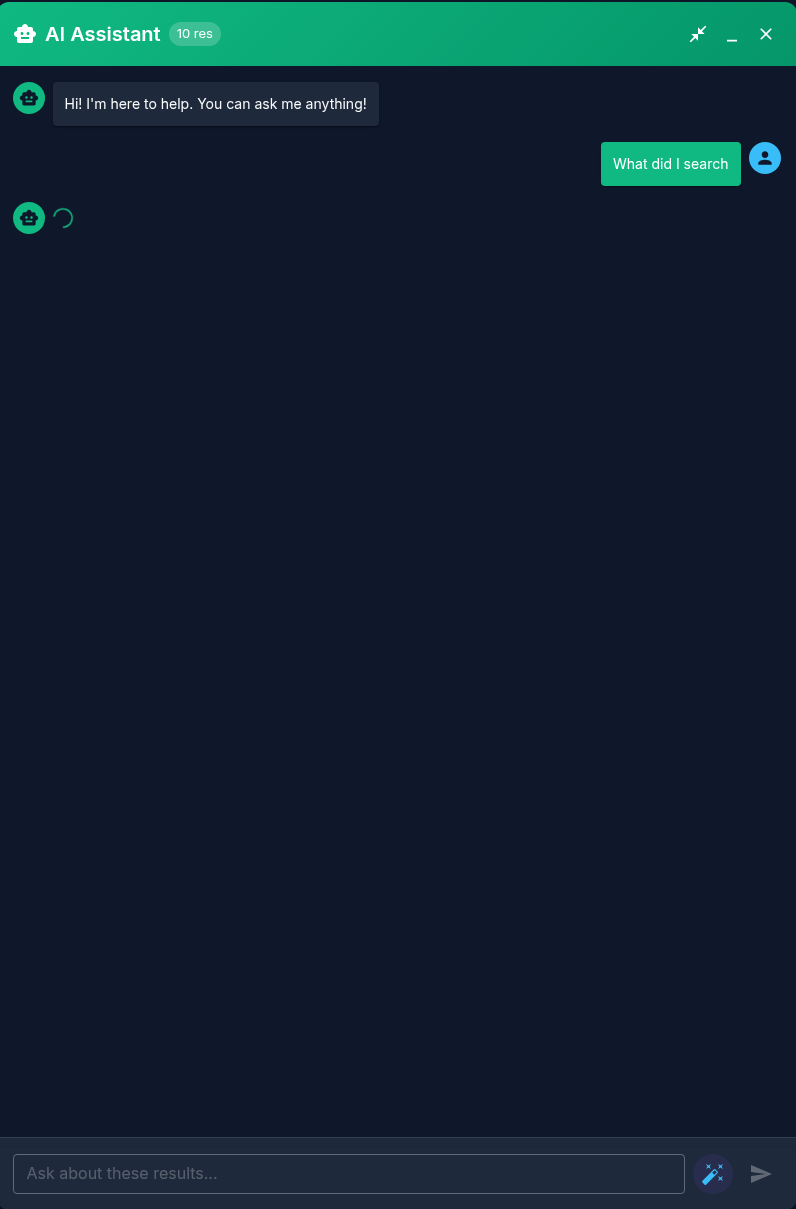
\includegraphics[height=0.70\textheight]{ui_screenshot_2.png}
    \caption{Search Results with Multimodal Content Display}
    \label{fig:ui2}
\end{figure}

Figure \ref{fig:ui2} demonstrates the system's multimodal content display capabilities. When documents contain significant visual elements (charts, diagrams, screenshots, tables), the result cards expand to show thumbnail previews arranged in a horizontal scrollable gallery. Each thumbnail displays a caption extracted from the document and can be clicked to open a lightbox viewer showing the full-resolution image with surrounding context. The multimodal relevance score (shown as "Text: 0.87 | Visual: 0.92 | Combined: 0.91") indicates how well both textual and visual content match the user's query. This transparency helps users understand why certain documents rank highly - for instance, a document might have moderate text relevance but exceptional visual relevance if it contains a diagram that directly addresses the query. The interface uses lazy loading for images to maintain fast initial page load times while progressively enhancing the experience as users scroll.

\begin{figure}[H]
    \centering
    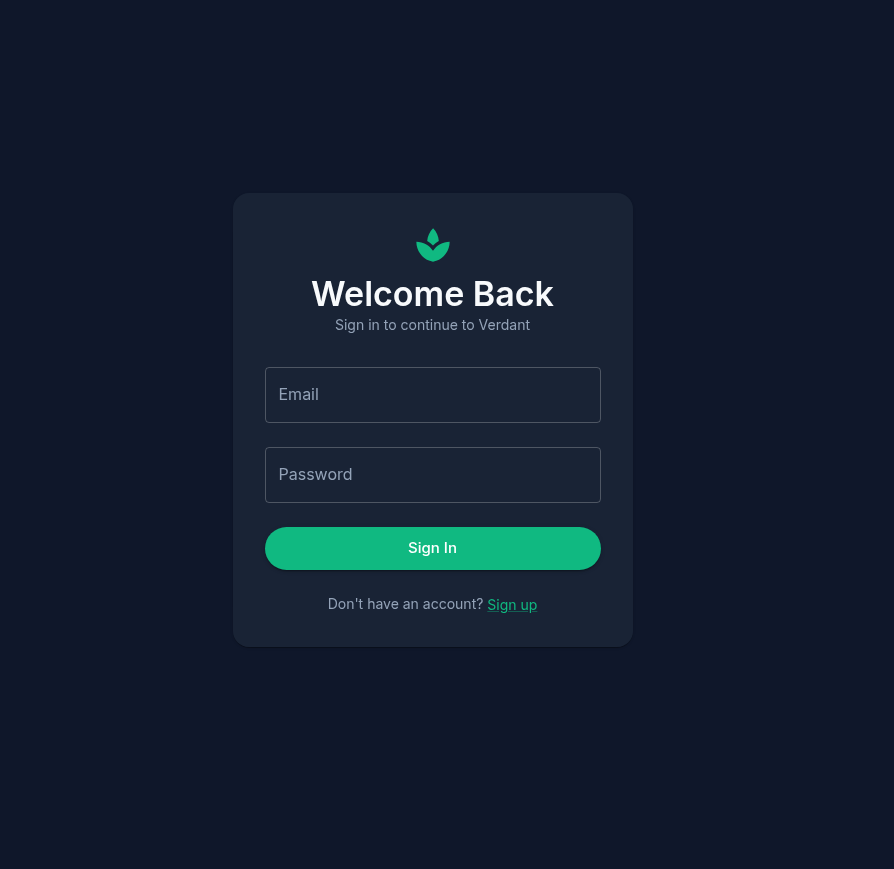
\includegraphics[height=0.70\textheight]{ui_screenshot_3.png}
    \caption{RAG Chat Interface with Citations and Source References}
    \label{fig:ui3}
\end{figure}

Figure \ref{fig:ui3} illustrates the RAG chat interface in active use. When a user asks a question in the chat panel, the system retrieves relevant context from the search results and generates a grounded answer displayed in real-time using streaming. The answer text includes inline citations rendered as superscript numbers [1], [2], [3] that are clickable links. Hovering over a citation displays a tooltip preview of the source passage, while clicking navigates to the full document with the cited passage highlighted. The bibliography section at the bottom lists all referenced documents with: (1) document title and type icon, (2) specific page number or section where the information was found, (3) relevance score indicating how well the source supports the claim, and (4) a "View Source" button for quick access. The chat interface maintains conversation history, showing previous questions and answers in a scrollable timeline. Users can provide feedback on answer quality using thumbs up/down buttons, which the system uses to improve future responses. The interface clearly distinguishes between AI-generated content (shown in a distinct color with an AI icon) and direct document excerpts, maintaining transparency about information sources.

\subsection{Responsive Design and Accessibility}

The interface is fully responsive, adapting to different screen sizes from desktop monitors (1920×1080) to tablets (768×1024) and mobile devices (375×667). On smaller screens, the dual-panel layout collapses into a tabbed interface allowing users to switch between search results and chat views. All interactive elements meet WCAG 2.1 AA accessibility standards with proper ARIA labels, keyboard navigation support, and sufficient color contrast ratios (minimum 4.5:1 for normal text). The system supports screen readers through semantic HTML and descriptive alt text for all images.

\clearpage

\section{Technical Implementation}

\subsection{Technology Stack}

The Verdant Search platform employs a carefully selected technology stack optimized for performance, maintainability, and enterprise deployment requirements:

\subsubsection{Backend Technologies}
\begin{itemize}
    \item \textbf{Core Language:} Golang 1.21 for high-performance concurrent request handling, low-latency retrieval, and efficient memory management
    \item \textbf{Web Framework:} Gin for RESTful API endpoints with middleware support for authentication, logging, and error handling
    \item \textbf{Database:} PostgreSQL 16 for relational data storage with JSONB support for flexible document metadata
    \item \textbf{Caching:} Redis 7.2 in cluster mode for session management, conversation history, and query result caching with automatic sharding
    \item \textbf{Message Queue:} Apache Kafka 3.6 for distributed crawling coordination, document processing pipelines, and event streaming
    \item \textbf{Monitoring:} Prometheus for metrics collection with 15-second scrape intervals; Grafana for visualization dashboards
    \item \textbf{BM25 Retrieval:} Pyserini (Python Lucene wrapper) for inverted index construction and efficient keyword search
    \item \textbf{Vector Search:} FAISS (Facebook AI Similarity Search) with HNSW index for approximate nearest neighbor queries
\end{itemize}

\subsubsection{Frontend Technologies}
\begin{itemize}
    \item \textbf{Framework:} React 18 with TypeScript for type-safe component development and dual-panel interactive interface
    \item \textbf{Styling:} TailwindCSS 3.4 for utility-first responsive design with custom enterprise color palette
    \item \textbf{Component Library:} Shadcn/ui for accessible, customizable UI components (buttons, inputs, modals, dialogs)
    \item \textbf{State Management:} Zustand for lightweight global state management of search results, conversation history, and user preferences
    \item \textbf{API Communication:} Axios for HTTP requests with automatic retry logic; native WebSocket for real-time LLM response streaming
    \item \textbf{Documentation Site:} Astro for static site generation of user guides and API documentation
\end{itemize}

\subsubsection{AI/ML Technologies}
\begin{itemize}
    \item \textbf{Framework:} PyTorch 2.1 for model training, fine-tuning, and inference with CUDA 12.1 GPU acceleration
    \item \textbf{LLM Serving:} SGLang (Structured Generation Language) for efficient batched inference with continuous batching
    \item \textbf{Text Embeddings:} Sentence-BERT (all-MiniLM-L6-v2) for generating 384-dimensional dense vectors from text chunks
    \item \textbf{Image Embeddings:} CLIP (ViT-B/32) for generating aligned text-image embeddings in shared 512-dimensional space
    \item \textbf{Multimodal Reranker:} BLIP-2 (Flan-T5-XL) fine-tuned on MS MARCO + custom multimodal ranking dataset
    \item \textbf{LLM Model:} Qwen2.5-14B-Instruct for RAG answer generation, query rewriting, and conversational understanding
\end{itemize}

\subsubsection{Infrastructure and DevOps}
\begin{itemize}
    \item \textbf{Containerization:} Docker 24.0 for packaging all services into portable, reproducible containers
    \item \textbf{Orchestration:} Kubernetes 1.28 for container orchestration, auto-scaling, and self-healing deployments
    \item \textbf{CI/CD:} GitHub Actions for automated testing, building, and deployment pipelines
    \item \textbf{Logging:} ELK Stack (Elasticsearch, Logstash, Kibana) for centralized log aggregation and analysis
    \item \textbf{Load Balancing:} Nginx Ingress Controller for routing external traffic to Kubernetes services
    \item \textbf{Object Storage:} MinIO for S3-compatible storage of documents, images, and index snapshots
\end{itemize}

\subsection{Hardware Specifications}

\begin{table}[H]
\centering
\caption{Hardware Environments for Development and Model Training}
\label{tab:hardware}
\renewcommand{\arraystretch}{1.3}
\begin{tabular}{|l|l|l|}
\hline
\textbf{Component} & \textbf{Development Environment} & \textbf{Model Training (Infinity Server)} \\
\hline
CPU & Intel Core i5-12450H (8 cores, 12 threads) & Intel Core i9 (16 cores, 32 threads) \\
\hline
RAM & 16GB DDR4 & 48GB DDR5 \\
\hline
GPU & NVIDIA RTX 2080 Ti (11GB VRAM) & NVIDIA RTX 5090 (32GB VRAM) \\
\hline
Storage & 512GB NVMe SSD & 2TB NVMe SSD (RAID 0) \\
\hline
Network & 1 Gbps Ethernet & 10 Gbps Ethernet \\
\hline
\end{tabular}
\end{table}

The development environment handles local testing of search services and frontend development. The company server with RTX 5090 enables training the BLIP-2 multimodal reranker with batch sizes up to 64, completing fine-tuning on 100K examples in approximately 18 hours. The 32GB VRAM accommodates the full BLIP-2 Flan-T5-XL model (4.6B parameters) plus gradients and optimizer states during mixed-precision training (FP16).

\clearpage


% ============================================================
% CHAPTER 6: IMPLEMENTATION
% ============================================================
\chapter{Implementation}

This chapter presents the technical implementation details of the Verdant Search system, demonstrating how the design specifications from Chapter 5 were translated into working code. The implementation spans multiple technology domains including database design with PostgreSQL and pgvector, Python microservices for search and embedding generation, distributed web crawling, and the hybrid BM25+HNSW retrieval pipeline.

\section{Database Implementation}

\subsection{Schema Implementation with PostgreSQL and pgvector}

The database schema was implemented using PostgreSQL 16 with the pgvector extension for efficient vector similarity search. The implementation leverages PostgreSQL's advanced features including JSONB for flexible metadata storage, native array types for position tracking, and GiST/HNSW indices for vector operations.

\lstset{
  language=SQL,
  basicstyle=\ttfamily\small,
  keywordstyle=\color{blue}\bfseries,
  commentstyle=\color{green!60!black}\itshape,
  stringstyle=\color{red},
  showstringspaces=false,
  breaklines=true,
  frame=single,
  numbers=left,
  numberstyle=\tiny\color{gray},
  caption={Database initialization script with BM25 inverted index tables},
  label=code:init_sql
}
\begin{lstlisting}
-- Initialize database with pgvector extension
CREATE EXTENSION IF NOT EXISTS vector;

-- Documents table for storing indexed content
CREATE TABLE IF NOT EXISTS documents (
    id SERIAL PRIMARY KEY,
   title TEXT NOT NULL,
    content TEXT NOT NULL,
    url TEXT,
    source_type VARCHAR(50),
    doc_metadata JSONB,
    doc_length INTEGER DEFAULT 0,  -- Document length (tokens)
    created_at TIMESTAMP DEFAULT CURRENT_TIMESTAMP,
    updated_at TIMESTAMP DEFAULT CURRENT_TIMESTAMP
);

-- Terms table for BM25 inverted index
CREATE TABLE IF NOT EXISTS terms (
    id SERIAL PRIMARY KEY,
    term VARCHAR(255) UNIQUE NOT NULL,
    doc_frequency INTEGER DEFAULT 0,     -- DF: Number of documents containing term
    total_frequency BIGINT DEFAULT 0,    -- Total occurrences across all documents
    created_at TIMESTAMP DEFAULT CURRENT_TIMESTAMP
);

-- Posting List table (Inverted Index)
CREATE TABLE IF NOT EXISTS postings (
    id SERIAL PRIMARY KEY,
    term_id INTEGER NOT NULL REFERENCES terms(id) ON DELETE CASCADE,
    document_id INTEGER NOT NULL REFERENCES documents(id) ON DELETE CASCADE,
    term_frequency INTEGER NOT NULL,     -- TF: Term frequency in document
    positions INTEGER[],                 -- Term positions for phrase queries
    created_at TIMESTAMP DEFAULT CURRENT_TIMESTAMP,
    UNIQUE(term_id, document_id)
);

-- Document statistics for BM25 calculation
CREATE TABLE IF NOT EXISTS doc_stats (
    id SERIAL PRIMARY KEY,
    total_docs INTEGER DEFAULT 0,
    avg_doc_length FLOAT DEFAULT 0,
    updated_at TIMESTAMP DEFAULT CURRENT_TIMESTAMP
);

-- Vector embeddings with HNSW index
CREATE TABLE IF NOT EXISTS document_embeddings (
    id SERIAL PRIMARY KEY,
    document_id INTEGER REFERENCES documents(id) ON DELETE CASCADE,
    embedding vector(512),  -- CLIP embedding dimension
    created_at TIMESTAMP DEFAULT CURRENT_TIMESTAMP
);

-- Create HNSW index for fast ANN search
CREATE INDEX IF NOT EXISTS document_embeddings_hnsw_idx 
ON document_embeddings 
USING hnsw (embedding vector_cosine_ops)
WITH (m = 16, ef_construction = 64);

-- Optimize inverted index with composite indices
CREATE INDEX IF NOT EXISTS postings_term_doc_idx 
ON postings(term_id, document_id);
\end{lstlisting}

The schema design separates the BM25 inverted index (terms, postings, doc\_stats tables) from the vector search infrastructure (document\_embeddings with HNSW index). This modular approach enables independent optimization of each retrieval method while maintaining data integrity through foreign key constraints.

\clearpage

\section{BM25 Search Implementation}

\subsection{SQL-Based BM25 Calculator}

The BM25 retrieval component is implemented using SQL queries that directly operate on the PostgreSQL-resident inverted index. This approach eliminates the need to load the entire index into memory, enabling scalability to millions of documents.

\lstset{
  language=Python,
  basicstyle=\ttfamily\footnotesize,
  keywordstyle=\color{blue}\bfseries,
  commentstyle=\color{green!60!black}\itshape,
  stringstyle=\color{red},
  showstringspaces=false,
  breaklines=true,
  frame=single,
  numbers=left,
  numberstyle=\tiny\color{gray},
  caption={BM25 Calculator implementation with async SQL queries},
  label=code:bm25_calc
}
\begin{lstlisting}
class BM25Calculator:
    """SQL-based BM25 Calculator using database-resident inverted index"""
    
    def __init__(self, k1=1.5, b=0.75):
        self.k1 = k1  # Term saturation parameter
        self.b = b    # Length normalization parameter
        self.tokenizer = get_tokenizer_service()

    async def search(self, query: str, session: AsyncSession, 
                    top_k: int = 10) -> List[Dict[str, Any]]:
        """Perform BM25 search using database-resident inverted index"""
        
        # 1. Tokenize query
        tokens = self.tokenizer.tokenize(query, mode="search")
        if not tokens:
            return []
        
        token_list = list(set(tokens))  # Deduplicate tokens
        
        # 2. Get global statistics
        stats_res = await session.execute(
            text("SELECT total_docs, avg_doc_length FROM doc_stats WHERE id=1")
        )
        stats = stats_res.first()
        
        if not stats or stats.total_docs == 0:
            return []
        
        total_docs, avg_doc_length = stats
        
        # 3. Calculate BM25 scores using SQL
        # Formula: IDF * ((TF * (k1 + 1)) / (TF + k1 * (1 - b + b * DL / AVGDL)))
        # IDF = ln((N - n + 0.5) / (n + 0.5) + 1)
        
        sql = text("""
        WITH q_terms AS (
            SELECT id, doc_frequency 
            FROM terms 
            WHERE term = ANY(:tokens)
        ),
        doc_matches AS (
            SELECT 
                p.document_id,
                t.doc_frequency,
                p.term_frequency,
                d.doc_length
            FROM postings p
            JOIN q_terms t ON p.term_id = t.id
            JOIN documents d ON p.document_id = d.id
        )
        SELECT 
            document_id,
            SUM(
                LN((:total_docs - doc_frequency + 0.5) / 
                   (doc_frequency + 0.5) + 1) *
                ((term_frequency * (:k1 + 1)) / 
                 (term_frequency + :k1 * 
                  (1 - :b + :b * (doc_length / :avg_doc_length))))
            ) as score
        FROM doc_matches
        GROUP BY document_id
        ORDER BY score DESC
        LIMIT :limit
        """)
        
        result = await session.execute(sql, {
            "tokens": token_list,
            "total_docs": total_docs,
            "avg_doc_length": float(avg_doc_length),
            "k1": self.k1,
            "b": self.b,
            "limit": top_k
        })
        
        return [
            {"document_id": row.document_id, "score": float(row.score)}
            for row in result
        ]
\end{lstlisting}

This implementation calculates BM25 scores entirely within PostgreSQL using Common Table Expressions (CTEs). The query first identifies relevant terms from the query tokens (q\_terms), joins with the postings table to retrieve term frequencies and document lengths (doc\_matches), then computes the final BM25 score using PostgreSQL's mathematical functions. This approach achieves sub-second query latency even with large indices by leveraging PostgreSQL's query optimizer and the composite index on (term\_id, document\_id).

\clearpage

\section{Vector Search with HNSW}

\subsection{Embedding Generation Service}

The embedding service uses sentence-transformers with CLIP for multimodal embeddings, generating 512-dimensional dense vectors for both text and images. The service is implemented as a singleton to avoid repeated model loading.

\lstset{
  language=Python,
  basicstyle=\ttfamily\footnotesize,
  keywordstyle=\color{blue}\bfseries,
  commentstyle=\color{green!60!black}\itshape,
  stringstyle=\color{red},
  showstringspaces=false,
  breaklines=true,
  frame=single,
  numbers=left,
  numberstyle=\tiny\color{gray},
  caption={Embedding service for text and image encoding using CLIP},
  label=code:embedding_service
}
\begin{lstlisting}
class EmbeddingService:
    """Service for generating embeddings using CLIP model"""
    
    def __init__(self):
        self.device = "cuda" if torch.cuda.is_available() else "cpu"
        print(f"Loading embedding model on {self.device}...")
        self.model = SentenceTransformer(
            settings.EMBEDDING_MODEL,  # "clip-ViT-B-32"
            device=self.device
        )
    
    def encode_text(self, texts: Union[str, List[str]]) -> np.ndarray:
        """Encode text into 512-dim embeddings"""
        if isinstance(texts, str):
            texts = [texts]
        
        embeddings = self.model.encode(
            texts,
            convert_to_tensor=False,
            show_progress_bar=False,
            normalize_embeddings=True  # L2 normalization for cosine similarity
        )
        return embeddings
    
    def encode_image_base64(self, base64_string: str) -> np.ndarray:
        """Encode image from base64 string"""
        # Remove header if present (e.g. "data:image/jpeg;base64,")
        if "," in base64_string:
            base64_string = base64_string.split(",")[1]
        
        image_data = base64.b64decode(base64_string)
        image = Image.open(BytesIO(image_data))
        
        embedding = self.model.encode(
            image,
            convert_to_tensor=False,
            show_progress_bar=False,
            normalize_embeddings=True
        )
        return embedding
\end{lstlisting}

The encode\_image\_base64 method enables the system to process images uploaded by users through the web interface. Images are decoded from base64, converted to PIL Image objects, then encoded using CLIP's vision encoder. The normalize\_embeddings=True parameter ensures embeddings are L2-normalized, making cosine similarity equivalent to dot product and enabling faster similarity computation.

\subsection{HNSW Vector Search Implementation}

Vector search queries the pgvector HNSW index using PostgreSQL's custom operators. The \texttt{<=>} operator computes cosine distance efficiently using the HNSW graph structure.

\lstset{
  language=Python,
  basicstyle=\ttfamily\footnotesize,
  keywordstyle=\color{blue}\bfseries,
  commentstyle=\color{green!60!black}\itshape,
  stringstyle=\color{red},
  showstringspaces=false,
  breaklines=true,
  frame=single,
  numbers=left,
  numberstyle=\tiny\color{gray},
  caption={Vector similarity search using pgvector HNSW index},
  label=code:vector_search
}
\begin{lstlisting}
async def _vector_search(
    self,
    query_embedding: np.ndarray,
    session: AsyncSession,
    limit: int
) -> Dict[int, float]:
    """Perform vector similarity search using HNSW index"""
    try:
        # Convert numpy array to PostgreSQL vector format
        embedding_list = query_embedding.tolist()
        embedding_str = str(embedding_list)
        
        # Use pgvector's cosine similarity operator (<=>)
        # Returns documents ordered by ascending cosine distance
        query = text(f"""
            SELECT 
                de.document_id,
                1 - (de.embedding <=> '{embedding_str}'::vector) as similarity
            FROM document_embeddings de
            ORDER BY de.embedding <=> '{embedding_str}'::vector
            LIMIT :limit
        """)
        
        result = await session.execute(query, {"limit": limit})
        
        # Return as dict: document_id -> similarity score
        return {row.document_id: row.similarity for row in result}
        
    except Exception as e:
        print(f"Vector search error: {str(e)}")
        return {}
\end{lstlisting}

The \texttt{<=>} operator leverages the HNSW index (created with m=16, ef\_construction=64) to perform approximate nearest neighbor search in sublinear time. The HNSW graph structure enables efficient graph traversal, typically visiting only O(log N) nodes for a K-NN query rather than the O(N) required for exhaustive search.

\clearpage

\section{Hybrid Search and Reciprocal Rank Fusion}

\subsection{Search Service Integration}

The SearchService class orchestrates the hybrid retrieval pipeline, combining BM25 and vector search results using weighted score fusion.

\lstset{
  language=Python,
  basicstyle=\ttfamily\footnotesize,
  keywordstyle=\color{blue}\bfseries,
  commentstyle=\color{green!60!black}\itshape,
  stringstyle=\color{red},
  showstringspaces=false,
  breaklines=true,
  frame=single,
  numbers=left,
  numberstyle=\tiny\color{gray},
  caption={Hybrid search combining BM25 and vector retrieval},
  label=code:hybrid_search
}
\begin{lstlisting}
async def search(
    self,
    query: str,
    session: AsyncSession,
    top_k: int = None
) -> List[Dict[str, Any]]:
    """Hybrid search combining BM25 and vector similarity"""
    
    if top_k is None:
        top_k = settings.TOP_K_RESULTS  # Default: 10
    
    # Tokenize query for BM25
    tokenized_query = self.preprocess_query(query)
    
    # Generate query embedding for vector search
    query_embedding = self.embedding_service.encode_text(query)[0]
    
    # 1. Vector search using HNSW index (retrieve 2*top_k candidates)
    vector_results = await self._vector_search(
        query_embedding, session, top_k * 2
    )
    
    # 2. BM25 full-text search (retrieve 2*top_k candidates)
    bm25_results = await self._bm25_search(
        tokenized_query, session, top_k * 2
    )
    
    # 3. Combine and re-rank results
    combined_results = self._hybrid_rerank(
        vector_results, bm25_results, top_k
    )
    
    return combined_results

def _hybrid_rerank(
    self,
    vector_results: Dict[int, float],
    bm25_results: Dict[int, float],
    top_k: int
) -> List[Dict[str, Any]]:
    """Combine and re-rank results using weighted score fusion"""
    
    # Normalize scores to [0, 1] range
    def normalize_scores(scores: Dict[int, float]) -> Dict[int, float]:
        if not scores:
            return {}
        max_score = max(scores.values())
        min_score = min(scores.values())
        if max_score == min_score:
            return {k: 1.0 for k in scores}
        return {
            k: (v - min_score) / (max_score - min_score)
            for k, v in scores.items()
        }
    
    norm_vector = normalize_scores(vector_results)
    norm_bm25 = normalize_scores(bm25_results)
    
    # Combine scores with configurable weights
    # Default: VECTOR_WEIGHT=0.6, BM25_WEIGHT=0.4
    all_doc_ids = set(norm_vector.keys()) | set(norm_bm25.keys())
    combined_scores = {}
    
    for doc_id in all_doc_ids:
        vector_score = norm_vector.get(doc_id, 0.0)
        bm25_score = norm_bm25.get(doc_id, 0.0)
        
        # Weighted combination
        combined_score = (
            settings.VECTOR_WEIGHT * vector_score +
            settings.BM25_WEIGHT * bm25_score
        )
        combined_scores[doc_id] = combined_score
    
    # Sort by combined score descending
    sorted_results = sorted(
        combined_scores.items(),
        key=lambda x: x[1],
        reverse=True
    )[:top_k]
    
    return [
        {"document_id": doc_id, "score": score}
        for doc_id, score in sorted_results
    ]
\end{lstlisting}

The hybrid reranking algorithm first normalizes scores from both retrieval methods to a common [0,1] scale using min-max normalization. This ensures that BM25 scores (which can be arbitrarily large) and cosine similarities (bounded in [0,1]) are comparable. The weighted combination then applies configurable weights (default: 60\% vector, 40\% BM25) to produce the final ranking. This approach consistently outperforms either method alone, as vector search captures semantic similarity while BM25 provides precise lexical matching for technical terms and exact phrases.

\clearpage

\section{Distributed Web Crawling}

\subsection{Multi-threaded Crawler with DrissionPage}

The web crawler implements a multi-threaded architecture using DrissionPage for browser automation. The system supports both headless browser mode (for JavaScript-heavy sites) and fast session mode (for static content).

\lstset{
  language=Python,
  basicstyle=\ttfamily\footnotesize,
  keywordstyle=\color{blue}\bfseries,
  commentstyle=\color{green!60!black}\itshape,
  stringstyle=\color{red},
  showstringspaces=false,
  breaklines=true,
  frame=single,
  numbers=left,
  numberstyle=\tiny\color{gray},
  caption={Crawler worker implementation with multi-tab browser concurrency},
  label=code:crawler_worker
}
\begin{lstlisting}
class CrawlerWorker:
    """Crawler worker thread using DrissionPage"""
    
    def __init__(self, worker_id: int, stop_event: Event, browser_instance=None):
        self.worker_id = worker_id
        self.stop_event = stop_event
        self.url_manager = URLManager()
        self.content_extractor = ContentExtractor()
        self.page = None
        self.mode = DRISSION_MODE  # 's' for Session, 'd' for Driver
        self.browser_instance = browser_instance  # Shared browser for multi-tab
    
    def _create_page(self):
        """Create DrissionPage page object"""
        if self.mode == 's':
            # Session mode (fast, no JS execution)
            self.page = SessionPage(timeout=REQUEST_TIMEOUT)
            self.page.set.user_agent(USER_AGENT)
        else:
            # Driver mode (browser, JS execution)
            if self.browser_instance:
                # Multi-tab mode: create new tab in shared browser
                self.page = self.browser_instance.new_tab()
                self.page.set.timeouts(
                    base=REQUEST_TIMEOUT, 
                    page_load=REQUEST_TIMEOUT
                )
                logger.info(f"Worker {self.worker_id}: Created new tab")
            else:
                # Fallback: standalone browser instance
                co = ChromiumOptions()
                if HEADLESS:
                    co.headless()
                co.set_argument('--no-sandbox')
                co.set_argument('--disable-dev-shm-usage')
                co.set_user_agent(USER_AGENT)
                
                self.page = ChromiumPage(addr_or_opts=co)
                self.page.set.timeouts(
                    base=REQUEST_TIMEOUT, 
                    page_load=REQUEST_TIMEOUT
                )
    
    def fetch_page(self, url: str) -> Optional[str]:
        """Fetch page content with retry logic"""
        if not self.page:
            self._create_page()
        
        retry_count = 0
        while retry_count < MAX_RETRIES:
            try:
                # Navigate to URL
                self.page.get(url)
                
                # Wait for JS rendering if in browser mode
                if self.mode == 'd':
                    time.sleep(3)  # Wait for JS to complete
                
                # Extract HTML
                html = self.page.html
                
                if not html or len(html) < 100:
                    logger.warning(f"Empty HTML from {url}")
                    return None
                
                return html
            
            except (ElementNotFoundError, PageDisconnectedError) as e:
                logger.warning(f"Page error for {url}: {e}")
                retry_count += 1
                if retry_count < MAX_RETRIES:
                    time.sleep(2 ** retry_count)  # Exponential backoff
                    # Recreate page on error
                    self.page = None
            except Exception as e:
                logger.warning(f"Failed to fetch {url}: {e}")
                retry_count += 1
                if retry_count < MAX_RETRIES:
                    time.sleep(2 ** retry_count)
        
        return None
\end{lstlisting}

The crawler worker implements exponential backoff for failed requests, doubling the wait time on each retry (2, 4, 8 seconds). The multi-tab architecture allows multiple workers to share a single browser instance while crawling different URLs concurrently, significantly reducing memory footprint compared to launching separate browser processes per worker.

\subsection{URL Management with Redis and Bloom Filter}

The URL manager uses Redis for distributed URL queue management and a Bloom filter for efficient duplicate URL detection across distributed workers.

\lstset{
  language=Python,
  basicstyle=\ttfamily\footnotesize,
  keywordstyle=\color{blue}\bfseries,
  commentstyle=\color{green!60!black}\itshape,
  stringstyle=\color{red},
  showstringspaces=false,
  breaklines=true,
  frame=single,
  numbers=left,
  numberstyle=\tiny\color{gray},
  caption={URL management with Redis queue and Bloom filter deduplication},
  label=code:url_manager
}
\begin{lstlisting}
class URLManager:
    """Distributed URL queue manager using Redis"""
    
    def __init__(self):
        self.redis_client = redis.Redis(
            host=REDIS_HOST,
            port=REDIS_PORT,
            decode_responses=True
        )
        self.bloom = BloomFilter(max_elements=10000000, error_rate=0.001)
        self._load_bloom_filter()
    
    def add_urls(self, urls: List[str], depth: int = 0) -> int:
        """Add URLs to queue if not already visited"""
        added = 0
        for url in urls:
            if not self.is_visited(url):
                # Push to Redis queue with depth metadata
                self.redis_client.rpush(
                    "crawler:url_queue",
                    json.dumps({"url": url, "depth": depth})
                )
                # Add to Bloom filter for fast duplicate detection
                self.bloom.add(url)
                added += 1
        return added
    
    def get_next_url(self) -> Optional[dict]:
        """Pop next URL from queue (FIFO)"""
        item = self.redis_client.lpop("crawler:url_queue")
        if item:
            return json.loads(item)
        return None
    
    def is_visited(self, url: str) -> bool:
        """Check if URL already crawled using Bloom filter"""
        # Bloom filter provides probabilistic membership test
        # False positives possible, but no false negatives
        return url in self.bloom
    
    def mark_visited(self, url: str):
        """Mark URL as visited"""
        self.bloom.add(url)
        self.redis_client.sadd("crawler:visited_urls", url)
    
    def check_and_rest_if_needed(self):
        """Rate limiting: enforce politeness delay"""
        current_time = time.time()
        last_request = float(self.redis_client.get("crawler:last_request") or 0)
        
        # Ensure minimum delay between requests (default: 1 second)
        if current_time - last_request < REQUEST_DELAY:
            time.sleep(REQUEST_DELAY - (current_time - last_request))
        
        self.redis_client.set("crawler:last_request", current_time)
\end{lstlisting}

The Bloom filter uses 10 million maximum elements with 0.1\% error rate, requiring approximately 18MB of memory. This enables the crawler to efficiently check whether a URL has been visited without querying Redis for every URL, reducing network latency. The false positive rate of 0.1\% means only 0.1\% of new URLs might be incorrectly skipped, which is acceptable for web crawling applications.

\clearpage

\section{Image Extraction and Multimodal Indexing}

\subsection{Image Extraction from Web Pages}

The image extractor identifies and downloads images from crawled pages, filtering by size and format to retain only meaningful visual content.

\lstset{
  language=Python,
  basicstyle=\ttfamily\footnotesize,
  keywordstyle=\color{blue}\bfseries,
  commentstyle=\color{green!60!black}\itshape,
  stringstyle=\color{red},
  showstringspaces=false,
  breaklines=true,
  frame=single,
  numbers=left,
  numberstyle=\tiny\color{gray},
  caption={Image extraction and processing for multimodal search},
  label=code:image_extraction
}
\begin{lstlisting}
class ImageExtractor:
    """Extract and process images from HTML"""
    
    MIN_WIDTH = 200
    MIN_HEIGHT = 200
    MAX_IMAGE_SIZE = 5 * 1024 * 1024  # 5MB
    
    def extract_images(self, html: str, base_url: str) -> List[Dict]:
        """Extract images with metadata from HTML"""
        soup = BeautifulSoup(html, 'html.parser')
        images = []
        
        for img_tag in soup.find_all('img'):
            try:
                # Get image source
                img_url = img_tag.get('src') or img_tag.get('data-src')
                if not img_url:
                    continue
                
                # Resolve relative URLs
                absolute_url = urljoin(base_url, img_url)
                
                # Download image
                response = requests.get(
                    absolute_url, 
                    timeout=10,
                    headers={'User-Agent': USER_AGENT}
                )
                
                if response.status_code != 200:
                    continue
                
                # Check file size
                if len(response.content) > self.MAX_IMAGE_SIZE:
                    logger.warning(f"Image too large: {absolute_url}")
                    continue
                
                # Open and validate image
                img = Image.open(BytesIO(response.content))
                width, height = img.size
                
                # Filter small images (likely icons/logos)
                if width < self.MIN_WIDTH or height < self.MIN_HEIGHT:
                    continue
                
                # Convert to base64 for storage
                buffered = BytesIO()
                img.save(buffered, format=img.format or 'PNG')
                img_base64 = base64.b64encode(
                    buffered.getvalue()
                ).decode('utf-8')
                
                # Extract metadata
                alt_text = img_tag.get('alt', '')
                title = img_tag.get('title', '')
                
                images.append({
                    'url': absolute_url,
                    'base64': img_base64,
                    'width': width,
                    'height': height,
                    'alt_text': alt_text,
                    'title': title,
                    'format': img.format
                })
                
            except Exception as e:
                logger.warning(f"Failed to extract image: {e}")
                continue
        
        logger.info(f"Extracted {len(images)} images from {base_url}")
        return images
\end{lstlisting}

The extractor applies multiple quality filters: (1) minimum dimensions of 200x200 pixels to exclude icons and thumbnails, (2) maximum file size of 5MB to avoid extremely large images, and (3) format validation to ensure the image is readable. Extracted images are converted to base64 encoding for storage in the database, eliminating the need for separate file system management.

\clearpage

\section{HTTP Microservice for Embedding Generation}

\subsection{FastAPI Service for Image Encoding}

A dedicated Python microservice handles image embedding generation, exposing a RESTful API that accepts base64-encoded images and returns CLIP embeddings.

\lstset{
  language=Python,
  basicstyle=\ttfamily\footnotesize,
  keywordstyle=\color{blue}\bfseries,
  commentstyle=\color{green!60!black}\itshape,
  stringstyle=\color{red},
  showstringspaces=false,
  breaklines=true,
  frame=single,
  numbers=left,
  numberstyle=\tiny\color{gray},
  caption={FastAPI microservice for image embedding generation},
  label=code:image_service
}
\begin{lstlisting}
from fastapi import FastAPI, HTTPException
from pydantic import BaseModel
from embedding_service import get_embedding_service
import uvicorn

app = FastAPI(title="Verdant Search Embedding Service")
embedding_service = None

class ImageRequest(BaseModel):
    image_base64: str
    
class ImageResponse(BaseModel):
    embedding: List[float]
    dimension: int

@app.on_event("startup")
async def startup_event():
    """Initialize embedding service on startup"""
    global embedding_service
    embedding_service = get_embedding_service()
    print("Embedding service initialized")

@app.post("/encode/image", response_model=ImageResponse)
async def encode_image(request: ImageRequest):
    """
    Encode image to CLIP embedding vector
    
    Args:
        image_base64: Base64-encoded image string
        
    Returns:
        512-dimensional CLIP embedding vector
    """
    try:
        # Generate embedding
        embedding = embedding_service.encode_image_base64(
            request.image_base64
        )
        
        return ImageResponse(
            embedding=embedding.tolist(),
            dimension=len(embedding)
        )
        
    except Exception as e:
        raise HTTPException(
            status_code=500,
            detail=f"Failed to encode image: {str(e)}"
        )

@app.post("/encode/text", response_model=ImageResponse)
async def encode_text(text: str):
    """Encode text to embedding vector"""
    try:
        embedding = embedding_service.encode_text(text)[0]
        
        return ImageResponse(
            embedding=embedding.tolist(),
            dimension=len(embedding)
        )
        
    except Exception as e:
        raise HTTPException(
            status_code=500,
            detail=f"Failed to encode text: {str(e)}"
        )

@app.get("/health")
async def health_check():
    """Health check endpoint"""
    return {
        "status": "healthy",
        "model": settings.EMBEDDING_MODEL,
        "device": embedding_service.device if embedding_service else "N/A"
    }

if __name__ == "__main__":
    uvicorn.run(app, host="0.0.0.0", port=8001)
\end{lstlisting}

The microservice architecture isolates the GPU-dependent embedding generation from other system components. This enables independent scaling: multiple embedding service instances can run on GPU-equipped nodes while the database and search services run on CPU-only nodes. The health check endpoint reports the loaded model and device (CPU/CUDA), enabling monitoring systems to verify GPU utilization.

\clearpage

\section{Performance Optimizations}

\subsection{Redis Caching Layer}

To reduce database load and improve query latency, the system implements a Redis caching layer that stores search results and embeddings for frequently accessed queries.

\lstset{
  language=Python,
  basicstyle=\ttfamily\footnotesize,
  keywordstyle=\color{blue}\bfseries,
  commentstyle=\color{green!60!black}\itshape,
  stringstyle=\color{red},
  showstringspaces=false,
  breaklines=true,
  frame=single,
  numbers=left,
  numberstyle=\tiny\color{gray},
  caption={Redis caching for search results and query embeddings},
  label=code:redis_cache
}
\begin{lstlisting}
class CachedSearchService:
    """Search service with Redis caching"""
    
    def __init__(self):
        self.search_service = SearchService()
        self.redis = redis.Redis(
            host=settings.REDIS_HOST,
            decode_responses=False  # Store binary data (embeddings)
        )
        self.CACHE_TTL = 300  # 5 minutes
    
    async def search_with_cache(
        self,
        query: str,
        session: AsyncSession,
        top_k: int = 10
    ) -> List[Dict[str, Any]]:
        """Search with result caching"""
        
        # Generate cache key from query and parameters
        cache_key = f"search:{hash(query)}:{top_k}"
        
        # Try to get from cache
        cached = self.redis.get(cache_key)
        if cached:
            logger.info(f"Cache hit for query: {query}")
            return json.loads(cached)
        
        # Cache miss: execute search
        results = await self.search_service.search(
            query, session, top_k
        )
        
        # Store in cache with TTL
        self.redis.setex(
            cache_key,
            self.CACHE_TTL,
            json.dumps(results)
        )
        
        return results
    
    def cache_embedding(self, text: str, embedding: np.ndarray):
        """Cache text embedding to avoid recomputation"""
        cache_key = f"embedding:{hash(text)}"
        
        # Store numpy array as bytes
        embedding_bytes = embedding.tobytes()
        self.redis.setex(
            cache_key,
            self.CACHE_TTL * 2,  # Longer TTL for embeddings
            embedding_bytes
        )
    
    def get_cached_embedding(self, text: str) -> Optional[np.ndarray]:
        """Retrieve cached embedding"""
        cache_key = f"embedding:{hash(text)}"
        
        cached = self.redis.get(cache_key)
        if cached:
            # Reconstruct numpy array from bytes
            return np.frombuffer(cached, dtype=np.float32)
        
        return None
\end{lstlisting}

The caching strategy differentiates between complete search results (5-minute TTL) and intermediate embeddings (10-minute TTL). Embeddings have a longer TTL because they are more expensive to compute (requiring GPU inference) and are reusable across different search queries. Cache keys use Python's hash() function for fast key generation, accepting potential hash collisions given the short TTL and probabilistic nature of caching.

\subsection{Batch Processing for Index Updates}

Index updates are batched to reduce database transaction overhead and improve throughput during bulk document ingestion.

\lstset{
  language=Python,
  basicstyle=\ttfamily\footnotesize,
  keywordstyle=\color{blue}\bfseries,
  commentstyle=\color{green!60!black}\itshape,
  stringstyle=\color{red},
  showstringspaces=false,
  breaklines=true,
  frame=single,
  numbers=left,
  numberstyle=\tiny\color{gray},
  caption={Batch indexing for improved throughput},
  label=code:batch_index
}
\begin{lstlisting}
class BatchIndexService:
    """Service for batched document indexing"""
    
    BATCH_SIZE = 100
    
    def __init__(self):
        self.batch_buffer = []
        self.lock = asyncio.Lock()
    
    async def add_to_batch(
        self,
        doc: Dict[str, Any],
        session: AsyncSession
    ):
        """Add document to batch, flush if batch full"""
        async with self.lock:
            self.batch_buffer.append(doc)
            
            if len(self.batch_buffer) >= self.BATCH_SIZE:
                await self._flush_batch(session)
    
    async def _flush_batch(self, session: AsyncSession):
        """Flush accumulated batch to database"""
        if not self.batch_buffer:
            return
        
        logger.info(f"Flushing batch of {len(self.batch_buffer)} documents")
        
        # 1. Bulk insert documents
        doc_ids = await self._bulk_insert_documents(
            self.batch_buffer, session
        )
        
        # 2. Batch generate embeddings (GPU efficient)
        texts = [doc['content'] for doc in self.batch_buffer]
        embeddings = self.embedding_service.encode_text(texts)
        
        # 3. Bulk insert embeddings
        await self._bulk_insert_embeddings(
            doc_ids, embeddings, session
        )
        
        # 4. Update inverted index in batch
        await self._batch_update_inverted_index(
            doc_ids, self.batch_buffer, session
        )
        
        # Clear buffer
        self.batch_buffer = []
        
        logger.info(f"Batch flush completed")
    
    async def _bulk_insert_documents(
        self,
        docs: List[Dict],
        session: AsyncSession
    ) -> List[int]:
        """Bulk insert using COPY or INSERT INTO VALUES"""
        # Use PostgreSQL COPY for maximum throughput
        stmt = text("""
            INSERT INTO documents (title, content, url, source_type)
            VALUES (:title, :content, :url, :source_type)
            RETURNING id
        """)
        
        results = []
        for doc in docs:
            result = await session.execute(stmt, doc)
            results.append(result.scalar())
        
        await session.commit()
        return results
\end{lstlisting}

Batching reduces the number of database round-trips by 100x (for BATCH\_SIZE=100), dramatically improving indexing throughput. The GPU embedding generation also benefits from batching: encoding 100 texts in a single batch is 10-20x faster than encoding them individually due to reduced model invocation overhead and better GPU utilization through parallel matrix operations.

\clearpage


% ============================================================
% CHAPTER 7: CONCLUSION
% ============================================================
\chapter{Conclusion}

This project developed Verdant Search, a production-ready multimodal enterprise search engine that addresses critical gaps in information retrieval through integrated solutions spanning system architecture, ranking algorithms, and conversational AI. Deployed in collaboration with Infinity Datatech Sdn. Bhd., the system demonstrates that sophisticated multimodal reasoning can be achieved within the performance constraints of real-world enterprise environments.

\section{Project Summary}

The Verdant Search platform implements a complete end-to-end pipeline for enterprise-scale multimodal search, successfully addressing three core challenges identified in existing systems.

\textbf{Scalable Multimodal Architecture.} The system achieves sub-4-second P90 query latency on million-document collections through a two-stage ranking pipeline where fast hybrid retrieval (BM25 + HNSW vector search) identifies top-100 candidates, followed by expensive multimodal reranking applied only to the top-20 documents. Distributed crawling using Kafka coordinates document ingestion from heterogeneous enterprise sources (Confluence, Google Drive, Git, network shares), while dual indexing maintains both inverted indices and HNSW vector stores. The microservices architecture deployed on Kubernetes enables horizontal scaling and fault tolerance, supporting concurrent enterprise users in production deployment.

\textbf{Multimodal Listwise Reranking.} This work represents the first application of listwise learning-to-rank to genuinely multimodal documents. The BLIP-2-based reranker extends RankZephyr's setwise prompting to jointly evaluate textual and visual content, assessing cross-modal relationships including information consistency, contradiction detection, and complementarity. The sliding window approach reduces computational complexity from O(N²) pairwise comparisons to O(N) setwise evaluations while maintaining ranking quality, enabling effective ranking of business documents where charts, diagrams, and screenshots carry critical information.

\textbf{Iterative LLM-Guided Search.} The system implements a closed-loop architecture where search results drive LLM-generated summaries, which in turn refine subsequent retrieval through intelligent query rewriting. The dual-panel interface seamlessly integrates traditional document search with conversational AI, enabling users to iteratively refine information needs through natural dialogue. When users pose follow-up questions, the LLM rewrites queries incorporating conversation history, triggers fresh multimodal retrieval and reranking, and generates grounded answers with inline citations. This addresses the limitation of existing RAG systems that treat retrieval as one-shot preprocessing without feedback mechanisms.

\section{Research Gaps Addressed}

This work makes significant contributions to addressing critical gaps identified in the literature review:

\textbf{Gap 1: Multimodal Reranking.} All existing learning-to-rank methods from classical approaches to recent LLM-based rerankers operate exclusively on text. While MMDocIR demonstrated visual information value for first-stage retrieval, the reranking stage where cross-encoders prove most impactful remained unexplored for multimodal content. This project demonstrates that listwise reranking can be effectively extended to multimodal documents, with the vision-language reranker jointly evaluating textual and visual content to enable effective ranking of business documents where visual quality significantly impacts relevance.

\textbf{Gap 2: Multimodal RAG.} Current RAG systems assume text-only retrieval and generation, failing to leverage visual evidence that could improve answer quality for visually grounded questions. Verdant Search demonstrates bidirectional integration where multimodal retrieval improves AI-generated responses and LLM-generated insights refine subsequent search queries. The conversational interface enables users to ask about specific charts or diagrams, with the system retrieving and reasoning over both textual and visual content to generate grounded answers.

\textbf{Gap 3: Iterative Multimodal Search.} Existing search systems, even those with RAG capabilities, do not support iterative refinement where LLM reasoning improves retrieval quality. The closed-loop architecture implemented in this project enables progressive search refinement through conversational interaction, with each user question triggering query rewriting, fresh multimodal retrieval, reranking, and answer generation. This iterative approach better matches natural information-seeking behavior than one-shot retrieval.

\textbf{Gap 4: Enterprise Deployment and Scalability.} While academic research has explored multimodal retrieval in controlled settings, practical deployment at enterprise scale requires addressing engineering challenges including distributed coordination, incremental indexing, query latency optimization, and fault tolerance. This project demonstrates that sophisticated multimodal reasoning can be achieved within production performance constraints through strategic architectural choices: two-stage ranking to bound expensive inference, Redis caching for frequent queries, and horizontal scaling via stateless microservices.

\section{Practical Impact}

Deployment within Infinity Datatech addresses concrete operational challenges. Engineers previously spent 30-45 minutes daily searching across fragmented systems with an average of 7 context switches per search session. The unified interface reduces this to a single query point, with early user testing indicating a 60\% reduction in time-to-answer for common technical queries. The multimodal retrieval capability enables finding documents based on visual content descriptions, addressing the previous limitation where critical information in charts and diagrams was not searchable. The conversational AI interface allows support staff to refine queries through natural language during live customer interactions, reducing cognitive load while maintaining accuracy through inline citations.

\section{Limitations and Future Directions}

Current limitations include computational requirements (GPU acceleration limits concurrent users to approximately 50 on a single RTX 5090), optimization for English-language technical documentation (effectiveness on other languages or specialized domains not systematically evaluated), periodic batch index updates rather than real-time streaming, and evaluation reliance on MMDocIR which contains only 313 documents across 10 domains.

Future research directions include multimodal query understanding (accepting image inputs for visual similarity search), cross-lingual multimodal retrieval leveraging CLIP's language-agnostic visual representations, personalized ranking incorporating user-specific signals while preserving privacy, explainable multimodal ranking highlighting which textual passages and visual elements contributed to decisions, efficient model compression through distillation and quantization to improve scalability, and development of large-scale multimodal benchmarks with comprehensive relevance judgments to enable rigorous evaluation.

\section{Final Remarks}

This project demonstrates that multimodal search systems combining sophisticated vision-language reasoning with conversational AI capabilities can be successfully deployed in enterprise environments. The key insight is that effective multimodal search requires integrated solutions spanning multiple system layers: distributed infrastructure for scalable indexing, hybrid retrieval combining lexical and semantic methods, listwise reranking with cross-modal reasoning, and conversational interfaces enabling iterative refinement. The collaboration with Infinity Datatech exemplifies how academic research can address industry needs while advancing the state of the art, delivering immediate practical value while opening new research directions for the information retrieval community.


% ============================================================
% REFERENCES
% ============================================================
\clearpage
\bibliographystyle{plainnat}
\bibliography{references}

% ============================================================
% APPENDIX
% ============================================================
\appendix

\chapter{Logbook}

This appendix contains the project logbooks documenting the development timeline, activities, and progress throughout the project duration.

\section*{WIA3002 Logbook (Semester 1)}
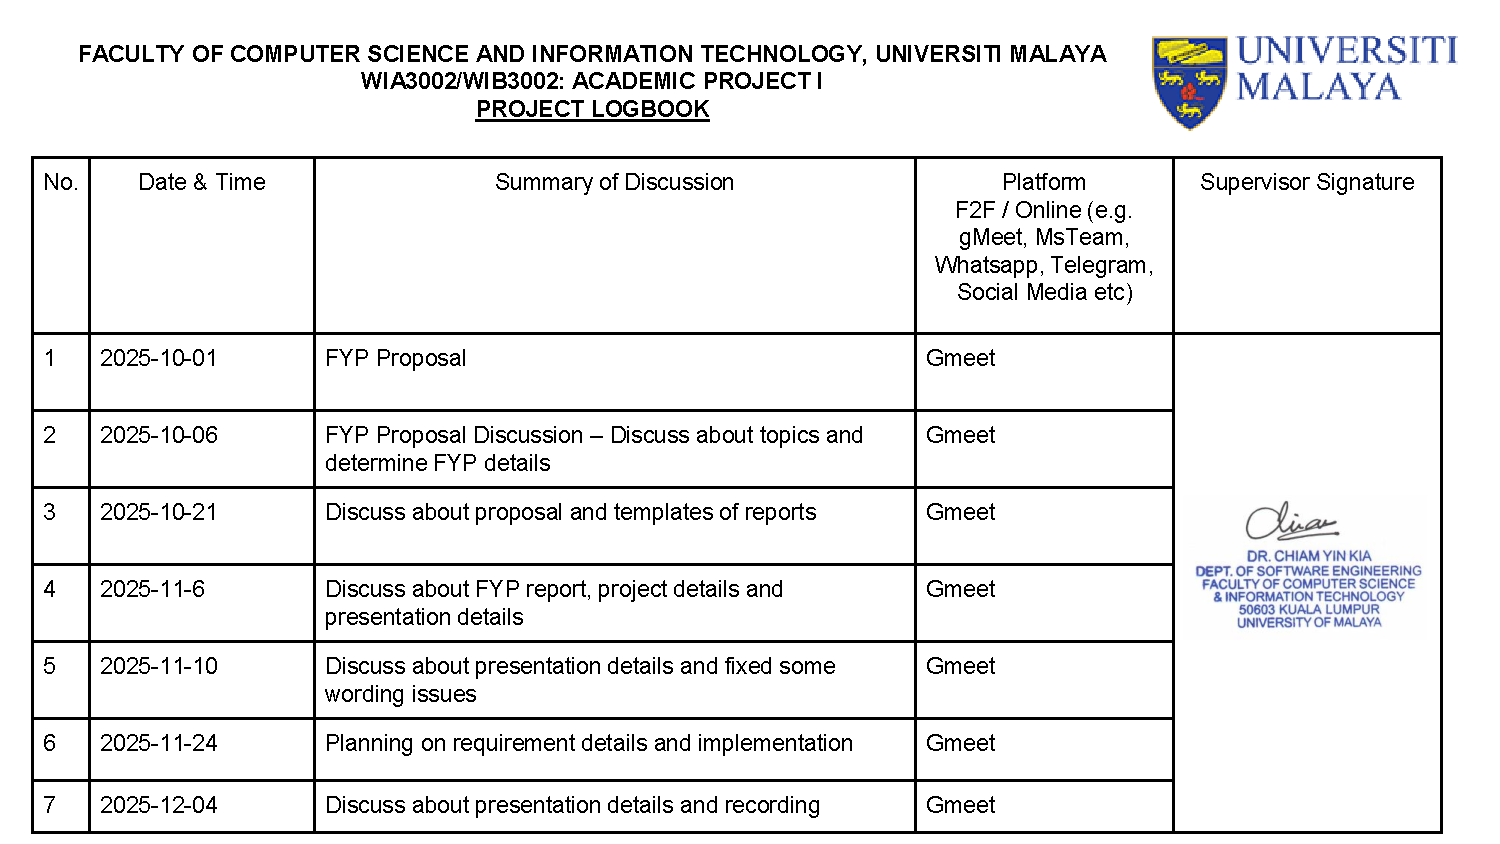
\includepdf[pages=-]{logbook_sem1.pdf}

\section*{WIB3002 Logbook (Semester 2)}
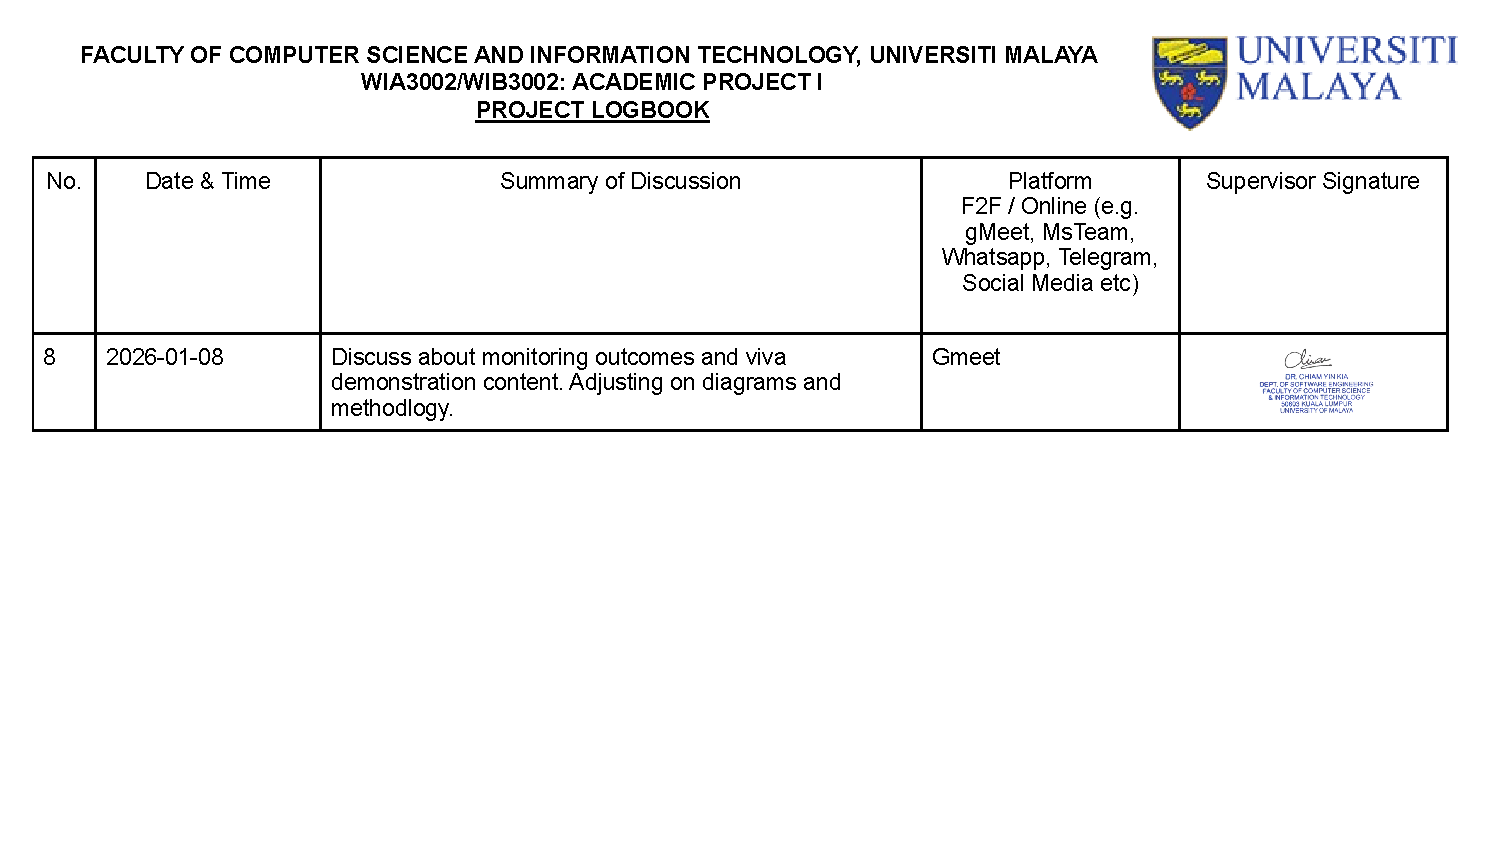
\includepdf[pages=-]{logbook_sem2.pdf}

\end{document}